% !TeX program = pdflatex
% ---------------------------------------------------------------------------
% Durable7 -- The Persistent Data Structure Field Guide
%
% A single-document tour of every data structure in the Durable7 repository.
%
% Build:  latexmk -pdf durable7-data-structures.tex
%
% SPDX-License-Identifier: MIT-0
% ---------------------------------------------------------------------------

\documentclass[11pt,twoside,openright]{book}

% --- Encoding, language, fonts --------------------------------------------
\usepackage[T1]{fontenc}
\usepackage[utf8]{inputenc}
\usepackage[english]{babel}
\usepackage{libertinus}
\usepackage[varqu,varl,scaled=0.95]{inconsolata}
\usepackage{microtype}
\usepackage{textcomp}
\usepackage{amsmath}
\usepackage{amssymb}

% --- Page geometry ---------------------------------------------------------
\usepackage[
  paperwidth=7in, paperheight=9.25in,
  inner=0.95in, outer=0.78in,
  top=0.95in, bottom=1.05in,
  headsep=16pt, footskip=30pt
]{geometry}

% --- Graphics, color, boxes ----------------------------------------------
\usepackage[table]{xcolor}
\usepackage{tikz}
\usetikzlibrary{arrows.meta,positioning,calc,fit,backgrounds,shapes.geometric,
                decorations.pathreplacing,decorations.pathmorphing,patterns}
\usepackage[most]{tcolorbox}
\tcbuselibrary{skins,breakable}
\usepackage{booktabs}
\usepackage{tabularx}
\usepackage{array}
\usepackage{longtable}
\usepackage{enumitem}
\usepackage{listings}
\usepackage{caption}
\usepackage{float}
\usepackage{needspace}
\usepackage{makeidx}
\makeindex

% --- Palette ---------------------------------------------------------------
\definecolor{d7ink}      {HTML}{16243C} % deep navy -- headings, body accents
\definecolor{d7copper}   {HTML}{A8562B} % warm accent -- rules, caveats
\definecolor{d7teal}     {HTML}{176E6E} % cool accent -- links, contracts
\definecolor{d7slate}    {HTML}{5A6779} % muted text
\definecolor{d7rule}     {HTML}{C9CFDA} % hairlines
\definecolor{d7paper}    {HTML}{F7F5F0} % box fill, warm
\definecolor{d7mist}     {HTML}{EEF2F6} % box fill, cool
\definecolor{d7sun}      {HTML}{F6EEE2} % box fill, caveat
\definecolor{d7leaf}     {HTML}{3E6B4A} % code strings
\definecolor{d7plum}     {HTML}{6B3A6B} % code keywords 2

% --- Cover palette ----------------------------------------------------------
% The cover runs a separate gray-olive-khaki range from the interior. Keeping it
% scoped means the mark can be retuned without restyling 133 pages of body text.
\definecolor{d7coverink}  {HTML}{262B21} % near-black olive -- cover title
\definecolor{d7coverdeep} {HTML}{3D4632} % deep olive -- structural strokes
\definecolor{d7coverolive}{HTML}{5D6B41} % olive -- mid strokes
\definecolor{d7coversage} {HTML}{75894C} % sage -- the live path
\definecolor{d7coverlime} {HTML}{A6B87A} % pale sage -- glow
\definecolor{d7coverkhaki}{HTML}{AFA372} % khaki -- retained versions
\definecolor{d7covergray} {HTML}{7C8478} % gray-green -- muted rule, subtitle
\definecolor{d7coverhaze} {HTML}{E9E9DD} % pale khaki-gray -- node fill
\definecolor{d7covermoss} {HTML}{F1F2E7} % lightest wash -- halo

% --- Hyperlinks ------------------------------------------------------------
\usepackage[
  colorlinks=true,
  linkcolor=d7ink,
  urlcolor=d7teal,
  citecolor=d7teal,
  pdftitle={Durable7: The Persistent Data Structure Field Guide},
  pdfauthor={The Durable7 Project},
  pdfsubject={Persistent and authenticated data structures},
  pdfkeywords={persistent data structures, CHAMP, HAMT, finger tree, RRB vector,
               Merkle search tree, zip tree, Patricia trie, rope},
  bookmarksnumbered=true,
  bookmarksopen=true,
  bookmarksopenlevel=1
]{hyperref}
\usepackage{bookmark}

% --- Sectioning style ------------------------------------------------------
\usepackage[explicit]{titlesec}

\titleformat{\part}[display]
  {\normalfont\sffamily\filcenter}
  {\color{d7copper}\large\scshape\partname~\thepart}
  {14pt}
  {\color{d7ink}\Huge\bfseries #1}
  [\vspace{10pt}{\color{d7copper}\rule{2.2cm}{1.4pt}}]

\titleformat{\chapter}[display]
  {\normalfont\sffamily}
  {\raggedleft\color{d7rule}\fontsize{62}{62}\selectfont\bfseries\thechapter}
  {-8pt}
  {\raggedright\color{d7ink}\huge\bfseries #1}
  [\vspace{7pt}{\color{d7copper}\rule{\textwidth}{1.1pt}}]
\titlespacing*{\chapter}{0pt}{-24pt}{28pt}

\titleformat{name=\chapter,numberless}[display]
  {\normalfont\sffamily}
  {}
  {0pt}
  {\raggedright\color{d7ink}\huge\bfseries #1}
  [\vspace{7pt}{\color{d7copper}\rule{\textwidth}{1.1pt}}]

\titleformat{\section}
  {\normalfont\sffamily\Large\bfseries\color{d7ink}}
  {\color{d7copper}\thesection}{0.7em}{#1}
\titleformat{\subsection}
  {\normalfont\sffamily\large\bfseries\color{d7ink}}
  {\color{d7copper}\thesubsection}{0.6em}{#1}
\titleformat{\subsubsection}
  {\normalfont\sffamily\normalsize\bfseries\color{d7slate}}
  {}{0pt}{#1}
\titlespacing*{\section}{0pt}{18pt plus 4pt minus 2pt}{7pt}
\titlespacing*{\subsection}{0pt}{14pt plus 3pt minus 2pt}{5pt}

% --- Running heads ---------------------------------------------------------
\usepackage{fancyhdr}
\fancypagestyle{d7main}{%
  \fancyhf{}
  \renewcommand{\headrulewidth}{0pt}
  \fancyhead[LE]{\sffamily\footnotesize\color{d7slate}\thepage\quad\textbar\quad\leftmark}
  \fancyhead[RO]{\sffamily\footnotesize\color{d7slate}\rightmark\quad\textbar\quad\thepage}
}
\fancypagestyle{plain}{%
  \fancyhf{}
  \renewcommand{\headrulewidth}{0pt}
  \fancyfoot[C]{\sffamily\footnotesize\color{d7slate}\thepage}
}
\renewcommand{\chaptermark}[1]{\markboth{\textsc{\lowercase{#1}}}{}}
\renewcommand{\sectionmark}[1]{\markright{\textsc{\lowercase{#1}}}}
\pagestyle{d7main}

% --- Typographic details ---------------------------------------------------
\setlength{\parskip}{0pt}
\setlength{\parindent}{1.2em}
\linespread{1.06}
% Long unbreakable \code{} spans in a 5.25in measure would otherwise overflow;
% let TeX buy the space from interword glue on the offending line instead.
\setlength{\emergencystretch}{2.5em}
\hbadness=2500
\vbadness=2500
\setlist{itemsep=2pt,parsep=1pt,topsep=5pt}
\setlist[itemize]{label=\textcolor{d7copper}{\small$\blacktriangleright$}}
\setlist[description]{font=\sffamily\bfseries\color{d7ink}}
\captionsetup{font=small,labelfont={sf,bf,color=d7copper},textfont={color=d7slate},
              justification=raggedright,singlelinecheck=false}
\renewcommand{\arraystretch}{1.18}
\arrayrulecolor{d7rule}

% --- Inline helpers --------------------------------------------------------
\newcommand{\code}[1]{\texorpdfstring{\textcolor{d7ink}{\texttt{#1}}}{#1}}
\newcommand{\lang}[1]{\textsf{\small #1}}
\newcommand{\term}[1]{\textit{#1}}
\newcommand{\bigoh}[1]{$\mathrm{O}(#1)$}

% Chapter epigraphs. \motto has no attribution line; \epigraph has one.
\newcommand{\motto}[1]{%
  \begingroup
  \vspace{-4pt}\hfill\begin{minipage}{0.80\textwidth}
    \raggedleft\itshape\color{d7slate}\small #1\par
  \end{minipage}\par\vspace{18pt}
  \endgroup}
\newcommand{\epigraph}[2]{%
  \begingroup
  \vspace{-4pt}\hfill\begin{minipage}{0.80\textwidth}
    \raggedleft\itshape\color{d7slate}\small #1\par
    \vspace{3pt}\normalfont\sffamily\scriptsize\upshape --- #2\par
  \end{minipage}\par\vspace{18pt}
  \endgroup}

% --- Code listings ---------------------------------------------------------
\lstdefinelanguage{Rust}{
  morekeywords={as,async,await,break,const,continue,crate,dyn,else,enum,extern,
    false,fn,for,if,impl,in,let,loop,match,mod,move,mut,pub,ref,return,self,Self,
    static,struct,super,trait,true,type,unsafe,use,where,while},
  morekeywords=[2]{Arc,Rc,Option,Result,Some,None,Ok,Err,Vec,String,usize,u32,u64,
    i32,i64,bool,str,Clone,Eq,Hash,BuildHasher,Send,Sync},
  sensitive=true, morecomment=[l]{//}, morecomment=[s]{/*}{*/}, morestring=[b]",
}
\lstdefinelanguage{TypeScript}{
  morekeywords={as,async,await,break,case,catch,class,const,continue,default,
    delete,do,else,export,extends,false,finally,for,from,function,if,implements,
    import,in,instanceof,interface,let,new,null,of,readonly,return,static,super,
    switch,this,throw,true,try,type,typeof,undefined,var,void,while,yield},
  morekeywords=[2]{string,number,boolean,bigint,unknown,never,any,Map,Set,Array,
    Promise,Iterable,Readonly},
  sensitive=true, morecomment=[l]{//}, morecomment=[s]{/*}{*/},
  morestring=[b]",morestring=[b]',
}
\lstdefinelanguage{Kotlin}{
  morekeywords={as,break,by,class,companion,const,continue,data,do,else,enum,
    false,for,fun,if,in,init,interface,internal,is,null,object,open,operator,
    override,package,private,public,return,sealed,super,this,throw,true,try,
    val,var,vararg,when,while},
  morekeywords=[2]{Int,Long,String,Boolean,List,Map,Set,Any,Unit,Nothing},
  sensitive=true, morecomment=[l]{//}, morecomment=[s]{/*}{*/},
  morestring=[b]",morestring=[b]',
}

\lstdefinestyle{d7}{
  basicstyle=\ttfamily\footnotesize\color{d7ink},
  keywordstyle=\color{d7ink}\bfseries,
  keywordstyle=[2]\color{d7plum},
  commentstyle=\itshape\color{d7slate},
  stringstyle=\color{d7leaf},
  showstringspaces=false,
  breaklines=true,
  breakatwhitespace=true,
  breakindent=1.6em,
  postbreak=\mbox{\textcolor{d7copper}{$\hookrightarrow$}\space},
  columns=fullflexible,
  keepspaces=true,
  tabsize=2,
  frame=leftline,
  framerule=1.4pt,
  rulecolor=\color{d7rule},
  framesep=9pt,
  xleftmargin=11pt,
  aboveskip=11pt,
  belowskip=8pt,
  upquote=true,
  % T1 turns << and >> into guillemets; shift operators must survive intact.
  literate={<<}{{\char60\char60}}2 {>>}{{\char62\char62}}2,
}
\lstset{style=d7}

% --- Callout boxes ---------------------------------------------------------
\newtcolorbox{contractbox}[1][The contract]{
  enhanced, breakable,
  colback=d7mist, colframe=d7teal, colbacktitle=d7mist,
  boxrule=0pt, leftrule=2.6pt,
  arc=0pt, outer arc=0pt,
  left=11pt, right=11pt, bottom=9pt, top=3pt,
  toptitle=7pt, bottomtitle=1pt, lefttitle=11pt,
  fonttitle=\sffamily\bfseries\footnotesize,
  coltitle=d7teal,
  title={#1},
}
\newtcolorbox{caveatbox}[1][Caveat]{
  enhanced, breakable,
  colback=d7sun, colframe=d7copper, colbacktitle=d7sun,
  boxrule=0pt, leftrule=2.6pt,
  arc=0pt, outer arc=0pt,
  left=11pt, right=11pt, bottom=9pt, top=3pt,
  toptitle=7pt, bottomtitle=1pt, lefttitle=11pt,
  fonttitle=\sffamily\bfseries\footnotesize,
  coltitle=d7copper,
  title={#1},
}
\newtcolorbox{glancebox}[1][At a glance]{
  enhanced, breakable,
  colback=white, colframe=d7rule,
  boxrule=0.8pt,
  arc=2pt, outer arc=2pt,
  left=11pt, right=11pt, top=15pt, bottom=9pt,
  fonttitle=\sffamily\bfseries\footnotesize,
  coltitle=d7slate,
  title={#1},
  attach boxed title to top left={xshift=11pt, yshift=-7pt},
  boxed title style={colback=white, boxrule=0pt, arc=0pt, left=3pt, right=3pt},
}
\newtcolorbox{asidebox}[1][Aside]{
  enhanced, breakable,
  colback=d7paper, colframe=d7paper, colbacktitle=d7paper,
  boxrule=0pt, arc=2pt,
  left=12pt, right=12pt, bottom=10pt, top=3pt,
  toptitle=8pt, bottomtitle=1pt, lefttitle=12pt,
  fonttitle=\sffamily\bfseries\footnotesize,
  coltitle=d7slate,
  title={#1},
}

% --- Reference tables that must break across pages --------------------------
% tabularx cannot break; longtable can. First argument is the fraction of
% \textwidth given to the label column.
\newenvironment{d7table}[1]
  {\par\vspace{3pt}\small
   \setlength{\LTpre}{4pt}\setlength{\LTpost}{4pt}
   \begin{longtable}{@{}%
     >{\raggedright\arraybackslash}p{#1\textwidth}%
     @{\hspace{10pt}}%
     >{\raggedright\arraybackslash}p{\dimexpr\textwidth-#1\textwidth-10pt\relax}@{}}}
  {\end{longtable}}

\newenvironment{d7tablethree}[2]
  {\par\vspace{3pt}\small
   \setlength{\LTpre}{4pt}\setlength{\LTpost}{4pt}
   \begin{longtable}{@{}%
     >{\raggedright\arraybackslash}p{#1\textwidth}%
     @{\hspace{8pt}}>{\raggedright\arraybackslash}p{#2\textwidth}%
     @{\hspace{8pt}}>{\raggedright\arraybackslash}p{\dimexpr\textwidth-#1\textwidth-#2\textwidth-16pt\relax}@{}}}
  {\end{longtable}}

% A compact "specimen card" used to open each structure's section.
% A specimen card is a run of label/value rows. Two side-by-side \parbox[t]es
% rather than a tabular: p-columns of differing font size do not reliably share
% a first baseline, and the label must sit level with the first line of prose.
\newcommand{\spec}[2]{%
  \par\noindent
  \parbox[t]{0.21\linewidth}{\raggedright\sffamily\bfseries\footnotesize
    \color{d7slate}\strut #1}%
  \hspace{9pt}%
  \parbox[t]{\dimexpr0.79\linewidth-9pt\relax}{\raggedright\strut #2}%
  \par\vspace{3.5pt}}
\newenvironment{specimen}[1][Specimen]
  {\begin{glancebox}[#1]\small\setlength{\parindent}{0pt}}
  {\end{glancebox}}

% Table helpers
\newcolumntype{L}[1]{>{\raggedright\arraybackslash}p{#1}}
\newcolumntype{Y}{>{\raggedright\arraybackslash}X}
\newcommand{\thead}[1]{\sffamily\bfseries\footnotesize\color{d7ink}#1}

% TikZ shared styles
\tikzset{
  d7node/.style={draw=d7ink, fill=white, rounded corners=1.5pt, inner sep=3pt,
                 font=\sffamily\scriptsize, minimum height=15pt},
  d7leafnode/.style={d7node, fill=d7mist},
  d7newnode/.style={d7node, draw=d7copper, fill=d7sun, very thick},
  d7ghost/.style={d7node, draw=d7rule, text=d7slate},
  d7edge/.style={-{Stealth[length=4pt]}, draw=d7slate, thin},
  d7newedge/.style={-{Stealth[length=4pt]}, draw=d7copper, thick},
  d7label/.style={font=\sffamily\scriptsize\color{d7slate}},
  d7cell/.style={draw=d7slate, thin, minimum width=13pt, minimum height=13pt,
                 font=\ttfamily\tiny, inner sep=0pt},
}

\begin{document}
\frenchspacing

% ===========================================================================
%  FRONT MATTER
% ===========================================================================
\frontmatter
\pagestyle{empty}

% --- Title page ------------------------------------------------------------
\begin{titlepage}
\centering
\vspace*{0.10\textheight}

% --- Cover mark -------------------------------------------------------------
% A version DAG whose subject is structural sharing: two live versions descend
% from one root and converge on a single retained node, which is therefore the
% only solid one and the only one inside a reticle. Every edge runs at exactly
% 45 degrees; the geometry is the point, so nothing here is freehand.
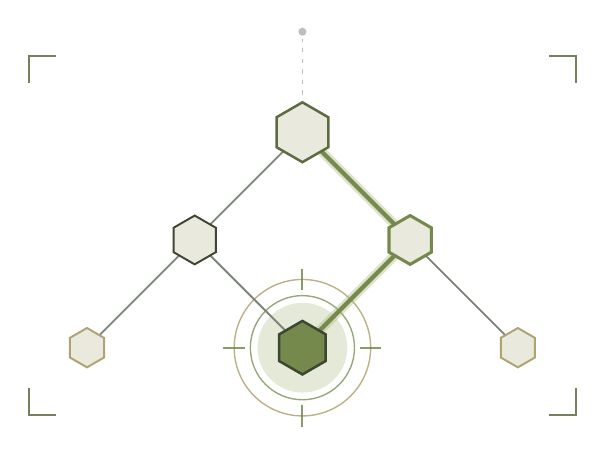
\begin{tikzpicture}[
  x=1.14cm, y=1.14cm,
  hex/.style={regular polygon, regular polygon sides=6, rotate=30,
              draw=d7coverdeep, fill=d7coverhaze, line width=0.7pt,
              inner sep=0pt, minimum size=#1},
  trace/.style={draw=d7covergray, line width=0.65pt,
                shorten >=2.2pt, shorten <=2.2pt},
  live/.style={draw=d7coversage, line width=1.5pt,
               shorten >=2.2pt, shorten <=2.2pt},
  halo/.style={draw=d7coverlime, line width=3.4pt, opacity=0.40,
               shorten >=2.2pt, shorten <=2.2pt},
]
  \coordinate (root) at (0,1.2);
  \coordinate (vl)   at (-1.2,0);
  \coordinate (vr)   at (1.2,0);
  \coordinate (fl)   at (-2.4,-1.2);
  \coordinate (sh)   at (0,-1.2);
  \coordinate (fr)   at (2.4,-1.2);

  % History continues above the root: the DAG is never rooted at the beginning.
  \draw[d7covergray, line width=0.6pt, opacity=0.5, dash pattern=on 1.6pt off 2.2pt]
    (0,1.62) -- (0,2.24);
  \fill[d7covergray, opacity=0.5] (0,2.32) circle (0.045);

  % Reticle around the shared node: two rings and four gap ticks.
  \fill[d7coverlime, opacity=0.30] (sh) circle (0.50);
  \draw[d7coversage, line width=0.5pt, opacity=0.75] (sh) circle (0.58);
  \draw[d7coverkhaki, line width=0.5pt, opacity=0.85] (sh) circle (0.76);
  \foreach \a in {0,90,180,270}
    { \draw[d7coversage, line width=0.7pt, opacity=0.85]
        ($(sh)+(\a:0.64)$) -- ($(sh)+(\a:0.88)$); }

  % Retained branches: still reachable from an older handle, never rewritten.
  \draw[trace] (root) -- (vl);
  \draw[trace] (vl) -- (fl);
  \draw[trace] (vl) -- (sh);
  \draw[trace] (vr) -- (fr);

  % The live path, glow beneath stroke.
  \draw[halo] (root) -- (vr);  \draw[halo] (vr) -- (sh);
  \draw[live] (root) -- (vr);  \draw[live] (vr) -- (sh);

  \node[hex=7.6mm, draw=d7coverolive, line width=0.9pt] at (root) {};
  \node[hex=6.2mm] at (vl) {};
  \node[hex=6.2mm, draw=d7coversage, line width=1.1pt] at (vr) {};
  \node[hex=5.0mm, draw=d7coverkhaki] at (fl) {};
  \node[hex=5.0mm, draw=d7coverkhaki] at (fr) {};
  \node[hex=6.8mm, draw=d7coverdeep, fill=d7coversage, line width=0.9pt] at (sh) {};

  % Close bracket frame: four L-marks, open on every side.
  \foreach \cx/\cy/\sx/\sy in {-3.05/2.05/1/-1, 3.05/2.05/-1/-1,
                               -3.05/-1.95/1/1, 3.05/-1.95/-1/1}
    { \draw[d7coverolive, line width=0.7pt, opacity=0.85]
        ($(\cx,\cy)+(0,{0.30*\sy})$) -- (\cx,\cy) -- ($(\cx,\cy)+({0.30*\sx},0)$); }
\end{tikzpicture}

\vspace{0.05\textheight}

{\ttfamily\fontsize{10}{13}\selectfont\color{d7coverolive}
 T\,H\,E\ \ D\,U\,R\,A\,B\,L\,E\,7\ \ F\,I\,E\,L\,D\ \ G\,U\,I\,D\,E\par}

\vspace{13pt}
{\color{d7coversage}\rule{0.10\textwidth}{1.6pt}}%
{\color{d7coverkhaki}\rule{0.24\textwidth}{1.6pt}}
\vspace{18pt}

{\sffamily\fontsize{34}{40}\selectfont\bfseries\color{d7coverink}
 Persistent\\Data Structures\par}

\vspace{16pt}

{\sffamily\fontsize{14}{20}\selectfont\color{d7covergray}
 Nine languages, one contract,\\forty-odd immutable collections\par}

\vspace{0.16\textheight}

{\sffamily\small\color{d7slate}
 A complete tour of the collections in the\\
 \textbf{Durable7} repository --- what each one is,\\
 why it exists, and when to reach for it.\par}

\vfill
{\ttfamily\footnotesize\color{d7covergray}
 Pre-release 0.1.0 \quad\textbullet\quad MIT No Attribution\par}
\end{titlepage}

% --- Colophon --------------------------------------------------------------
\thispagestyle{empty}
\null\vfill
\begin{flushleft}\small\color{d7slate}
\textbf{\sffamily Durable7: The Persistent Data Structure Field Guide}\\[6pt]
This document describes the collections implemented in the Durable7 repository.
It is a companion to --- not a replacement for --- the workspace API
specifications and public headers, which remain the normative source for
contracts, complexity, allocation behavior, and validation evidence.
Where this guide and a workspace specification disagree, the specification
wins and this guide has a bug.\\[10pt]
The repository ports every family to \textbf{C}, \textbf{C\texttt{++}},
\textbf{C\#}, \textbf{Haskell}, \textbf{Kotlin}, \textbf{OCaml},
\textbf{Python}, \textbf{Rust}, and \textbf{TypeScript}. Code samples are drawn
from whichever port makes the point most clearly; every behavior described in
the shared-contract sections holds in all nine unless the text says
otherwise.\\[10pt]
Set in Libertinus with Inconsolata for code; diagrams drawn in \textsc{Ti\emph{k}Z};
typeset with \LaTeX.\\[10pt]
Licensed \textbf{MIT No Attribution (MIT-0)}. Use it, fork it, ship it.
\end{flushleft}
\vspace{18pt}

% --- Contents --------------------------------------------------------------
\cleardoublepage
\pagestyle{plain}
\setcounter{tocdepth}{1}
{\hypersetup{linkcolor=d7ink}
 \renewcommand{\contentsname}{Contents}
 \tableofcontents}

% --- How to read -----------------------------------------------------------
\cleardoublepage
\pagestyle{d7main}
\chapter*{How to read this guide}
\addcontentsline{toc}{chapter}{How to read this guide}
\markboth{\textsc{how to read this guide}}{\textsc{how to read this guide}}

There are two honest ways to use a book about data structures. You can read it
straight through, which is what you want when you are trying to understand a
design space. Or you can open it at the one page that answers today's question,
which is what you want at 4pm on a Thursday. This guide is arranged so that both
work.

\bigskip
\noindent\textbf{\sffamily\color{d7ink}If you are reading straight through.}
Part~\ref{part:foundations} explains what persistence buys and what it costs,
and sets out the vocabulary that the rest of the book leans on --- policies,
representatives, no-op identity, failure atomicity. Nothing after it will quite
land without it. Parts~\ref{part:hash} through~\ref{part:authenticated} then walk
the families in the order a curious reader would want them: the hash trie first
(it is the substrate for a third of everything else), then sequences, then
ordered and priority collections, then the authenticated tier. Part~\ref{part:navigation}
covers cursors, which cut across every family. The appendices are reference
material.

\bigskip
\noindent\textbf{\sffamily\color{d7ink}If you are looking something up.}
Every structure gets a \emph{specimen card} --- a compact panel with its purpose,
its complexity, its policy requirements, and its nine-language spellings ---
followed by prose that explains the representation and the decisions inside it.
Appendix~\ref{app:complexity} is a single sorted complexity table across the
whole library. Appendix~\ref{app:names} is a name-to-name index across the nine
ports. The subject index at the back covers both concepts and identifiers.

\bigskip
\noindent\textbf{\sffamily\color{d7ink}Three kinds of panel appear throughout.}

\begin{contractbox}[The contract]
Normative behavior that every port upholds. If a port cannot honor one of
these, it says so explicitly in its own API notes rather than quietly differing.
\end{contractbox}

\begin{caveatbox}[Caveat]
The place where a claim stops being true. These are the paragraphs worth reading
twice --- most production surprises with persistent structures live exactly at
the edge of an amortization argument or a policy assumption.
\end{caveatbox}

\begin{asidebox}[Aside]
History, provenance, and the occasional road not taken. Skippable, but they are
where the design reasoning usually hides.
\end{asidebox}

\bigskip
\noindent\textbf{\sffamily\color{d7ink}A note on honesty.} This library is
unusually careful about the difference between a bound it can prove and a bound
it would like to have. Several structures ship as \emph{checkpoints}: the
observable semantics match the reference port exactly, but the representation is
simpler and the asymptotic claim is weaker. Wherever that is the case, this
guide says so in the same breath as the feature. A guide that only reported the
good news would be a worse guide.

% ===========================================================================
%  PART I -- FOUNDATIONS
% ===========================================================================
\mainmatter

\part{Foundations}
\label{part:foundations}

\chapter{What Persistence Buys}
\label{ch:persistence}

\motto{The old version is still there. That one sentence is the whole
library, and everything else is an argument about how to afford it.}

\noindent
Here is a small program, and a large idea hiding inside it.

\begin{lstlisting}[language={[Sharp]C}]
var v1 = PersistentHashMap<int, string>.Empty.SetItem(1, "one");
var v2 = v1.SetItem(2, "two");
var v3 = v2.SetItem(1, "uno");
\end{lstlisting}

\noindent
After three lines you are holding three maps. Not three references to one map
that has been mutated three times --- three genuinely independent collections,
each of which will answer questions about its own contents forever. \code{v1}
still has exactly one entry. \code{v2} still maps \code{1} to \code{"one"}. You
can hand \code{v1} to another thread while a third thread builds \code{v4} from
\code{v3}, and no lock is involved anywhere, because nothing that either thread
can see is ever written to again.

The obvious way to get that behavior is to copy the map on every update, and
the obvious problem with the obvious way is that it costs \bigoh{n} time and
\bigoh{n} space per edit. A library of persistent collections is, in essence, a
long and inventive answer to the question: \emph{how little can we copy and
still tell the truth?}

\section{Path copying, and the shape of an update}

The answer, in one picture, is Figure~\ref{fig:pathcopy}. Update-shaped
operations copy the nodes along the route from the root to the point of change
and reuse every other node by reference.\index{path copying} For a tree of branching factor $b$ and
$n$ elements, that is $\log_b n$ new nodes rather than $n$ --- for a 32-way trie
holding a million entries, four small nodes instead of a million entries.

\begin{figure}[htbp]
\centering
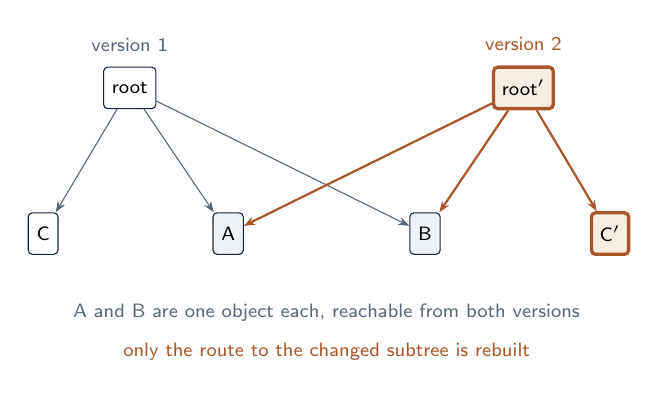
\begin{tikzpicture}[node distance=0pt]
  \node[d7node] (R)  at (-2.5, 0)    {root};
  \node[d7newnode] (R2) at ( 2.5, 0) {root$'$};
  \node[d7node] (C)  at (-3.6,-1.85) {C};
  \node[d7leafnode] (A) at (-1.25,-1.85) {A};
  \node[d7leafnode] (B) at ( 1.25,-1.85) {B};
  \node[d7newnode] (C2) at ( 3.6,-1.85) {C$'$};

  \draw[d7edge] (R) -- (C);
  \draw[d7edge] (R) -- (A);
  \draw[d7edge] (R) -- (B);
  \draw[d7newedge] (R2) -- (C2);
  \draw[d7newedge] (R2) -- (A);
  \draw[d7newedge] (R2) -- (B);

  \node[d7label, above=2pt of R]  {version 1};
  \node[d7label, above=2pt of R2, text=d7copper] {version 2};
  \node[d7label] at (0,-2.85) {A and B are one object each, reachable from both versions};
  \node[d7label, text=d7copper] at (0,-3.35) {only the route to the changed subtree is rebuilt};
\end{tikzpicture}
\caption{Path copying. Version~2 differs from version~1 in a single subtree.
The two nodes on the route to that subtree are freshly allocated (copper); every
other node is shared verbatim. Neither version can observe the other's
existence.}
\label{fig:pathcopy}
\end{figure}

Two consequences follow immediately, and both matter more than they look.

\textbf{Old versions cost almost nothing to keep.} Retaining \code{v1} does not
pin a second copy of the data; it pins the handful of nodes that later versions
replaced.\index{structural sharing} A hundred snapshots of a slowly changing map are cheaper than one
would guess and vastly cheaper than a hundred deep copies. This is what makes
undo stacks, audit trails, and time-travel debugging practical rather than
aspirational.

\textbf{Readers need no synchronization.} Every node reachable from a published
root is immutable, so a reader that has captured a root is reading a frozen
world. There is no torn read, no lock, no volatile fence in the read path, and
no window during which a concurrent writer can make a traversal observe half of
two different states. The synchronization problem does not get solved; it gets
deleted.

\section{The version DAG}

Because an update produces a new value rather than modifying an old one, nothing
forces versions into a line.\index{version DAG} Branch from \code{v2} twice and you get two
descendants that share \code{v2}'s structure and know nothing about each other
(Figure~\ref{fig:versiondag}). This is why persistent collections are the natural
substrate for editors, transactional stores, speculative execution, and any
system where ``what if'' has to be cheap.

\begin{figure}[htbp]
\centering
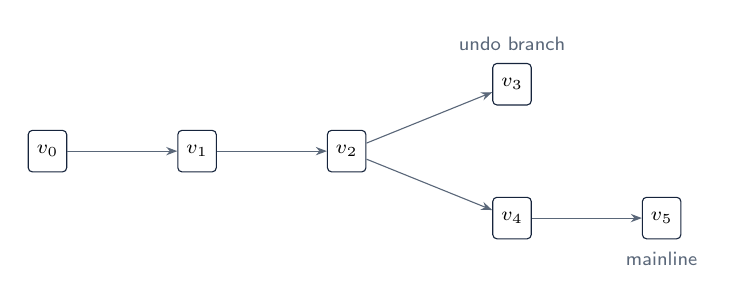
\begin{tikzpicture}
  \node[d7node] (v0) at (0,0)      {$v_0$};
  \node[d7node] (v1) at (1.9,0)    {$v_1$};
  \node[d7node] (v2) at (3.8,0)    {$v_2$};
  \node[d7node] (v3) at (5.9,0.85) {$v_3$};
  \node[d7node] (v4) at (5.9,-0.85){$v_4$};
  \node[d7node] (v5) at (7.8,-0.85){$v_5$};
  \draw[d7edge] (v0)--(v1); \draw[d7edge] (v1)--(v2);
  \draw[d7edge] (v2)--(v3); \draw[d7edge] (v2)--(v4); \draw[d7edge] (v4)--(v5);
  \node[d7label,above=1pt of v3] {undo branch};
  \node[d7label,below=1pt of v5] {mainline};
\end{tikzpicture}
\caption{Versions form a directed acyclic graph, not a sequence. Every node in
the picture is a live, complete collection.}
\label{fig:versiondag}
\end{figure}

That freedom has a price, and it is the single most important caveat in this
book.

\begin{caveatbox}[Amortization does not survive branching]
Amortized bounds are proved by a potential argument over \emph{one linear
history}: an expensive operation is paid for by cheap operations that preceded
it.\index{amortization!under branching} Branching breaks the argument. If a version sits just before an expensive
rebalance, and you branch from it $b$ times, each branch can trigger that same
rebalance, and the accumulated credit pays for exactly one of them. Potential
consumed by one child cannot pay for a sibling.

Durable7 therefore classifies every adaptive scheme before believing its
amortized claim. Constant-size promotion thresholds are safe --- re-branching
re-pays only \bigoh{1}. Schemes that do \bigoh{n} work at a threshold ---
relabeling, compaction, wholesale redistribution --- are not, and the library
either avoids them or states the worst case per produced version. Where a bound
holds only along a linear lineage, this guide says ``linear lineage''
explicitly.
\end{caveatbox}

\section{What it costs}

Persistent collections are not free, and pretending otherwise makes for a bad
guide. The honest ledger looks like this.

\begin{itemize}
\item \textbf{Allocation per update.} Every edit allocates its copied path. A
tight loop of point updates on a persistent map will allocate far more than the
same loop on a hash table. This is the motivation for the entire builder and
editing-session tier (Chapter~\ref{ch:lifecycle}).
\item \textbf{Indirection on reads.} A 32-way trie lookup is a handful of
pointer hops with good branch prediction, but it is still pointer hops. A flat
open-addressed table wins on a hot small map, every time.
\item \textbf{Cache behavior.} Node-based structures scatter. The library's
answer is chunking --- ropes hold runs of elements in contiguous leaves, RRB
vectors hold 32-element arrays, chunked bit sets hold 64-bit words --- so that
scans get array speed even though edits get tree behavior.
\item \textbf{Small collections lose.} The regime in which a persistent map
looks worst is the one most programs spend most of their time in: maps with
three entries. The library records a size-tiered representation as a strong idea
that is deliberately \emph{not} shipped, because it has not yet been justified
with benchmarks (Appendix~\ref{app:roads}).
\end{itemize}

\section{Where mutation is allowed}

A library that is honest about persistence has to be equally honest about its
exceptions. Durable7 confines mutation to four clearly labeled places, and
every one of them is documented as mutable wherever it appears:

\begin{description}
\item[Construction-only bulk builders] mutate unpublished trie nodes while
building a collection from a sequence, then freeze. Nothing observable is ever
mutated, because the nodes are not reachable until the freeze.
\item[One-way editing sessions] adopt a persistent root, accept a run of edits
under single ownership, and publish once. Publication consumes the session.
\item[The concurrent hash trie] is a genuinely mutable lock-free map whose
distinguishing feature is that \code{Snapshot()} is \bigoh{1}.
\item[\code{DabaLite}] is a mutable sliding-window aggregator. It is in the
library because it reuses the monoid vocabulary, not because it is persistent;
it explicitly is not.
\end{description}

\section{Why nine implementations}

Most collection libraries exist once, and a ``port'' is a family resemblance.
Here, semantic parity is the product. The same ordering rules, the same
first-representative retention, the same no-op identity, the same failure
atomicity, and --- for the authenticated tier --- the same bytes on the wire, in
C, C\texttt{++}, C\#, Haskell, Kotlin, OCaml, Python, Rust, and TypeScript.

The interesting part is what \emph{does not} have to match. Rust uses
\code{Arc} and forbids \code{unsafe}; C\# exposes \code{IReadOnlyList<T>};
OCaml returns \code{option} and \code{result}; C is type-erased with explicit
ownership and fallible allocators; Haskell keeps its sessions in \code{IO}.
Idioms are local. Semantics are not.

\begin{asidebox}[The checkpoint idea]
Nine simultaneous implementations of a subtle algorithm would normally mean nine
opportunities to quietly claim a bound nobody proved. Durable7's device for
avoiding that is the \term{checkpoint port}: a port that preserves the
observable API semantics and passes the same behavioral tests, while
documenting exactly which representation or asymptotic property it does
\emph{not} yet have.\index{checkpoint port} Most of the newer cursors are
checkpoints: the multimap's cursor resolves a rank by walking the grouped
flattening, so it is linear where the collection it navigates is logarithmic, and
its specification says so in the same table that gives every other row. Saying so
in the API notes is treated as part of shipping, not as an admission of failure
--- and a checkpoint is a debt with a name on it rather than a permanent
concession. Chapter~\ref{ch:laziness} follows one such debt, carried by five
ports at once, to the point where it was paid.
\end{asidebox}

\chapter{Laziness, and the Price of Persistence}
\label{ch:laziness}

\motto{Amortization is credit spent by the operations that come after.
Persistence lets a caller spend the same credit again, and again, out of the
same version. Memoization is what closes the account.}

\begin{specimen}[Specimen --- the memoized suspension]
\index{suspension!memoized}\index{laziness}\index{memoization}%
\spec{Purpose}{Make an amortized bound survive persistent branching, by deferring cascading work and charging every version that shares it at most once.}
\spec{Core}{A one-slot cell holding either a pending operation or its result. Forcing runs the operation and publishes the result back into the cell.}
\spec{Operations}{A closed set of deferred spine steps: push an overflow node into the middle from the front, push one from the back, concatenate two middles around regrouped nodes, and --- where reversal is a view --- mirror a middle.}
\spec{Complexity}{What it buys the finger tree: \bigoh{1} amortized endpoints and \bigoh{\log \min(n,m)} concatenation that stay true \emph{under branching}. Without it both collapse to \bigoh{\log n}.}
\spec{Mutability}{One write per cell, ever, and only after the deferred computation has succeeded.}
\spec{Ports}{All nine, each with its own publication primitive (Section~\ref{sec:nine-cells}). Haskell gets it from the language; the other eight build it by hand.}
\spec{Limits}{Pending chains reach $\Theta(n)$ links. Forcing them --- and releasing them --- must be iterative, never recursive.}
\end{specimen}

\noindent
Chapter~\ref{ch:persistence} closed its tour of the version DAG with a warning:
amortized bounds are proved over one linear history, and branching breaks the
proof. That warning was abstract, a rule for classifying adaptive schemes. This
chapter is what it looks like made concrete, because the structure it threatens
is the one a third of this library is built on.

\section{The credit that gets spent twice}

A finger tree earns its cheap ends from its digits (Chapter~\ref{ch:fingertree}).
Pushing onto a digit that has room is \bigoh{1}: the digit widens and nothing
else moves. Pushing onto a \emph{full} digit is not. Four items are regrouped
into a 2-3 node and pushed down into the middle, where they may meet another
full digit and cascade again, as far as the spine goes. Classic amortized
analysis absorbs this the way it absorbs a doubling array: the cheap pushes
between cascades deposit credit, the rare cascade spends it, the average is
constant. The argument is correct --- for a structure with one past.

Now keep an old version. Let $v$ sit exactly one push away from a cascade $k$
levels deep, and let a caller retain $v$ and push from it $b$ times. Each push
produces its own successor and each successor pays the whole cascade, because
the results are not shared --- only the input is. The aggregate is $\Theta(bk)$
where the bound promised $\Theta(b)$: credit deposited once, before $v$, and
spent $b$ times.\index{amortization!under persistence} Nothing about that
program is adversarial. It is an undo stack retrying from a checkpoint, a
speculative evaluator forking a candidate state a few dozen ways, an editor
keeping every keystroke --- the workloads persistent collections exist to serve.
A naive persistent finger tree does not deliver the \bigoh{1} ends it is famous
for. It delivers them to the last version anyone touched.

\section{Suspend, then memoize}

Hinze and Paterson's answer (\textit{JFP}, 2006) is not to make the cascade
cheaper. It is to not do it yet, and then to arrange that it is done at most
once. When a digit overflows, the overflowing middle is not rebuilt; it is
stored as an unevaluated computation --- a \term{suspension}. When some later
operation actually needs that middle, the computation runs and the result is
written back into the very cell that held it. Every version whose spine passes
through that node holds a reference to that one cell, so the first branch to
force it pays and every other branch reads the published result.

That is worth stating as a thesis rather than as a technique:
\textbf{laziness here is not an optimization; it is the correctness condition of
the amortization argument.} A strict finger tree is not a slower finger tree; it
is a different data structure with different bounds. Okasaki makes the general
form of the argument in \textit{Purely Functional Data Structures}: amortization
and persistence are reconciled by lazy evaluation with memoization and by
essentially nothing else, and the worst-case variants of the same structures are
then obtained by \emph{scheduling} the forced work, not by removing the
laziness.

Two restrictions keep this from turning the tree into a cloud of thunks. Only
the middle subtree of each deep node is suspended, so a tree of $n$ elements
carries $\Theta(\log n)$ suspensions rather than one per element; and within
them only the monoid's \code{combine} is ever deferred, because element measures
are computed eagerly at insertion and every node's size is strict at every
construction site. That second restriction is what keeps the promises of
Chapter~\ref{ch:measures} honest: reading the first element, the last element,
or the length invokes no policy callback at all, on any port, at any size.

\begin{contractbox}[What a suspension cell owes]
A cell is written at most once, and only \emph{after} the deferred computation
has succeeded. A measure policy that throws or raises mid-force therefore
publishes nothing: the cell stays pending, the force may be retried, and every
retained version remains valid --- the failure atomicity of
Chapter~\ref{ch:contract}, extended into the laziness machinery.

Pending operations are pure, so running one twice yields structurally identical
results. That is what makes a concurrent force benign: two threads may duplicate
the bounded computation, but they converge on one published value, and no reader
observes a partially initialized node or two different element sequences.
\end{contractbox}

\begin{figure}[htbp]
\centering
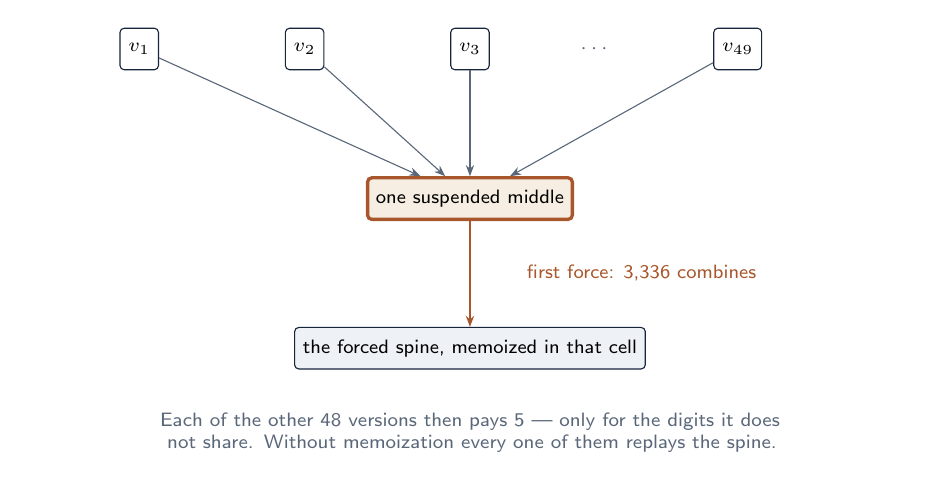
\begin{tikzpicture}[x=1mm,y=1mm]
  \node[d7node] (v1) at (-42,0) {$v_1$};
  \node[d7node] (v2) at (-21,0) {$v_2$};
  \node[d7node] (v3) at (  0,0) {$v_3$};
  \node[d7label] at (16,0) {$\cdots$};
  \node[d7node] (v49) at ( 34,0) {$v_{49}$};
  \node[d7newnode] (S) at (0,-19) {one suspended middle};
  \draw[d7edge] (v1) -- (S);
  \draw[d7edge] (v2) -- (S);
  \draw[d7edge] (v3) -- (S);
  \draw[d7edge] (v49) -- (S);
  \node[d7leafnode] (T) at (0,-38) {the forced spine, memoized in that cell};
  \draw[d7newedge] (S) -- (T);
  \node[d7label, anchor=west, text=d7copper] at (6,-28.5)
    {first force: 3{,}336 combines};
  \node[d7label, anchor=north, align=center, text width=110mm] at (0,-45)
    {Each of the other 48 versions then pays 5 --- only for the digits it does
     not share. Without memoization every one of them replays the spine.};
\end{tikzpicture}
\caption{Memoization under branching. Forty-nine versions retain the same
unforced spine. The suspension is a cell they share, not a computation each of
them owns, so the deferred work happens once and is read forty-eight times.
These are the numbers the library's probes assert.}
\label{fig:suspension}
\end{figure}

\section{Nine languages, nine publication primitives}
\label{sec:nine-cells}

In Haskell the compiler supplies all of this: a thunk is a memoized suspension,
and the tree is written the way the paper writes it. In the other eight
workspaces the cell has to be built by hand, and the interesting question is not
whether a strict language can do it --- it is what each language's atomic
publication primitive turns out to be.

\begin{d7tablethree}{0.13}{0.33}
\toprule
\thead{Language} & \thead{Suspension cell} & \thead{Note} \\
\midrule
C\#         & One field holding either the pending operation or the tree,
published by an \code{Interlocked} compare-exchange & The reference. A pending
\emph{push} reports its measure without forcing; a pending pop cannot, so the
node's measure is memoized separately. \\
C\texttt{++} & An atomic box over \code{shared\_ptr}, published by
compare-exchange & Cells force themselves without external locking. \\
C           & Hand-rolled memoized middle cells over reference counts & The
existence proof that this needs no runtime support at all. \\
Haskell     & The language & Native laziness; nothing to build. \\
\midrule
Rust        & \code{Arc} plus \code{OnceLock} & A lost race discards the
duplicate result. Also needs an iterative \code{Drop}. \\
Kotlin      & An \code{AtomicReference} over sealed operation classes,
published by \code{compareAndSet} & The JVM collector handles teardown. \\
OCaml       & One mutable field, written under the runtime lock & Native
\code{Lazy.t} deliberately not used --- see below. \\
TypeScript  & Plain field assignment & The one single-threaded workspace, where
assignment simply \emph{is} the atomic publication --- documented as such rather
than left looking like an oversight. \\
Python      & A thunk slot rewritten to its value under the GIL & \\
\bottomrule
\end{d7tablethree}

The four above the rule always had this; the five below received it in the
campaign of Section~\ref{sec:parity}. All nine publish identically: the result
enters the cell only once the deferred computation has returned.

\begin{caveatbox}[The one mutable cell in an immutable structure]
Chapter~\ref{ch:persistence} said a reader holding a root is reading a frozen
world, with no write in the read path. In the finger-tree spine that is very
nearly, but not exactly, true: the first read that needs a suspended middle both
computes and \emph{stores}. What survives is the part consumers depend on --- no
torn read, no lock, no observable state change, no traversal that sees half of
two versions. What does not survive is the literal claim of a write-free read
path, which is why eight of the nine ports reach for an atomic publication
primitive rather than a plain store. The user-visible consequence is stated
wherever it applies: reading a whole tree's measure is \bigoh{1} \emph{amortized},
not worst case, because the first such read on a freshly edited spine may force
a chain of suspensions. Endpoint reads and length never force.
\end{caveatbox}

\section{The chain that eats the stack}

Now run an ordinary loop: append $n$ elements and read nothing. Each overflow
suspends a push into a middle that is itself an unforced suspension, holding a
pending push into another. After the loop the spine carries a chain of pending
operations $\Theta(n)$ links long, none of it forced.

The natural implementation of a suspension is a closure capturing the next cell,
and forcing it is a call --- one stack frame per link. This is where a technique
that is correct on paper meets a machine, and the library learned it three times
in three different ways.

\textbf{Python made it immediate.} A default limit of a thousand frames turns a
few thousand appends into a stack overflow, which at least has the virtue of
failing in the first test run rather than in production.

\textbf{OCaml made it instructive.} ``The language already has laziness'' looks
like an exemption from the whole problem, and it is not: a direct experiment, run
before the OCaml core was designed, established that native \code{Lazy.force}
itself overflows on a chain 200,000 deep. \code{Lazy.t} was then banned from that
workspace's spine --- a port declining a language feature precisely because it
needs the property the feature is named after.

\textbf{Rust contributed a variant nobody planned for.} A chain that is never
forced still has to be \emph{released}. Under reference counting, dropping the
last handle to the head cell runs the destructor of its pending payload, which
drops the next cell, which drops the next: one frame per link again, on the
teardown path this time. A tracing collector hides this completely; reference
counting does not. Rust's suspension therefore implements an iterative
\code{Drop} that unlinks the chain with \code{Arc::into\_inner}.

The remedy is the same in every case, and older than any of them:
\term{defunctionalize} the suspension.\index{defunctionalization} Instead of a
closure, store the deferred operation as \emph{data} --- a sealed class, an enum,
a variant type --- drawn from a small closed set: push an overflow node into the
middle from the front, push one from the back, concatenate two middles around
already-regrouped nodes, and, in the three workspaces where whole-value reversal
is a lazy structural mirror (Chapter~\ref{ch:revdeque}), mirror a middle.
Forcing is then an explicit-stack interpreter over that data, and depth costs
heap rather than frames. Every rebuilt core forces a 200,000-element organically
built chain in its probe suite on every build; Rust drops one, unforced, as well.

How deep a suspension may nest is itself a design choice, and the reference
answers it differently. C\# forces the captured source \emph{when the pending
operation is created} --- the paper's own remark about forcing the middle
subtree in the recursive case of \code{cons} to avoid building a chain of
suspensions --- so a C\# cell is exactly one deferred step deep and the deepest
chain a force can meet is the height of the tree. Both realizations deliver the
same asymptotic bounds; they trade a bounded eager force at creation against an
unbounded lazy one later. One gap was recorded rather than papered over: the
three strict donor cores were never stress-tested against the same
200,000-deep force-and-release the five rebuilt cores now run, and that probe is
filed as open.

\section{The parity campaign}
\label{sec:parity}

For most of this library's life, everything above described four workspaces.

The discovery began with a small question during a port review: why did one
Python collection document a $\Theta(s \log n)$ endpoint update where the C\#
reference said \bigoh{s} amortized? The honest answer --- because Python's
substrate was not a finger tree --- prompted a survey of what each workspace's
substrate really was, and the survey immediately found worse. Rust's core module
described itself as a 2-3 finger tree, documented \bigoh{1} \code{front} and
\code{back} and \bigoh{\log \min} concatenation, and stored a node of
\code{\{ left, right, len, height, measure \}} --- a plain height-balanced binary
tree --- whose \code{front} recursed the entire left spine. The documentation was
not conservative. It was false.

Nine censuses then ran in parallel, one per workspace, reading node
representations and delivered bounds \emph{from the code} and treating every
documented bound as a claim to check. Four workspaces --- C\#, C, C\texttt{++},
Haskell --- carried the real lazy Hinze--Paterson structure. Five carried
height-balanced binary \term{join trees}\index{join tree} instead: AVL or
weight-balanced, one element per node, a measure cached at each node. A join tree
delivers the same \bigoh{\log n} interior operations and fundamentally cannot
deliver \bigoh{1} ends or \bigoh{\log \min} concatenation, having neither digits
nor laziness. Three of the five nevertheless \emph{called} themselves finger
trees, and two documented bounds their code did not deliver.

\begin{contractbox}[The parity principle]
Every language uses the same algorithms and the same data structures and offers
the same complexity guarantees, wherever that is possible at all. No fix may make
any delivered bound asymptotically worse. When one workspace delivers a
\emph{stronger} guarantee than the reference, that guarantee becomes the target
for every workspace where it is achievable. And where a bound depends on
laziness, strict languages implement memoized suspensions by hand --- which C\#,
C\texttt{++}, and C had already proven feasible here, including in plain C.
\end{contractbox}

All five cores were rebuilt in place: same module, same public API, checked
mechanically against the previous export lists, so every facade above them ---
deques, sorted collections, priority queues, interval trees, ropes, chunked bit
sets --- inherited the new bounds without a source change, and their existing
behavioral tests served as free regression harnesses.

\begin{d7tablethree}{0.24}{0.30}
\toprule
\thead{Operation} & \thead{Join-tree cores, before} & \thead{All nine cores,
now} \\
\midrule
first / last read & $\Theta(\log n)$ spine descent (Rust's docs claimed
\bigoh{1}) & \bigoh{1} worst case --- a digit field read \\
endpoint push / pop & $\Theta(\log n)$, worst \emph{and} amortized: joining
against a singleton rebuilds the spine & \bigoh{1} amortized, valid under
persistent branching; \bigoh{\log n} worst case per call \\
concatenation & \bigoh{\text{height difference}}, so appending a short run to a
long sequence paid the long sequence's height & \bigoh{\log \min(n,m)}
amortized --- the suspended middle recursion stops at the shallower operand \\
split / index / locate & \bigoh{\log n} & \bigoh{\log n}, unchanged --- the
no-regression rule \\
whole-value \code{Reverse} & $\Theta(n)$ rebuild through an array (Python,
TypeScript, OCaml) & \bigoh{1} --- a lazy structural mirror, the fourth deferred
operation \\
mixed-orientation concat & $\Theta(n+m)$ re-materialization (same three) &
\bigoh{\log \min}, structural: mirror the smaller operand lazily \\
\bottomrule
\end{d7tablethree}

The ``wherever possible at all'' clause was exercised twice, and both rulings
were written down so a later maintainer can revisit them with the original
reasoning in hand. One workspace's placeholder collections stored each version as
a flat sorted array --- \bigoh{1} rank-select, $\Theta(n)$ writes; since no
persistent structure is known that offers \bigoh{\log n} writes \emph{and}
\bigoh{1} select, rank-select regressed to the reference's \bigoh{\log n}, and
every affected interface says so. Separately, an append-only node arena shared by
two of the newer collections has a $\Theta(\sqrt M)$ allocation spike at block
boundaries; removing it would have cost permanent complexity in eight hot paths,
so the spike was kept and all seven arena ports made to document it identically
rather than let one quietly differ. A no-regression rule needs an escape valve
with a paper trail. These are it.

Equalizing \emph{upward} fired in a direction nobody planned. Python's first
lazy \code{Reverse} reused each mirrored node's cached measure, which is correct
only when \code{combine} commutes, and documented that as a caller obligation;
the TypeScript port instead recombined each mirrored summary in mirrored order
--- constant extra work per node, paid only when the reversal forces, correct
under \emph{every} monoid. That is strictly stronger, so Python was rewritten to
match the same day and OCaml was required to have the stronger shape from birth.

\section{Pinning a claim that tests cannot see}

The most transferable result of the whole campaign is one sentence:
\textbf{asymptotic claims are invisible to correctness tests.} A join tree passes
every behavioral test a finger tree passes. It returns the same elements in the
same order, preserves the same representatives, honors the same no-op identities,
fails atomically in the same places. Every suite in all five workspaces was green
on the wrong data structure.

So the library pins bounds the only way they can be pinned: with \term{counting
probes}.\index{counting probe} Every policy object a structure takes ---
comparator, measure, tag algebra --- has a counting variant, and the suites
assert against the counters rather than against a stopwatch: an exact call count
where the number is deterministic, and a size-independence equality plus a tight
budget where it is not. What fails is then arithmetic, not intuition. The
signature result of the campaign is that the five rebuilt cores produce
\emph{byte-identical} numbers.

\begin{d7table}{0.44}
\toprule
\thead{Probe} & \thead{Pinned result} \\
\midrule
512 endpoint pushes (256 at each end) onto a tree of 1{,}024, and onto one of
32{,}768 & exactly 340 \code{combine} calls --- \emph{the same number at both
sizes}, which is the amortized-\bigoh{1} claim written as an equality \\
Concatenating a 4{,}096-element tree with a singleton, and with a
1{,}024-element operand & 0 immediate combines, and 4 --- cost tracking the
smaller operand, not the height difference \\
A 10{,}000-append spine branched into 49 retained versions & 3{,}336 combines
when the first branch forces it; exactly 5 per branch for the other 48 \\
\code{front}, \code{back}, \code{length} & zero policy calls, at any size \\
\bottomrule
\end{d7table}

The third row is Figure~\ref{fig:suspension}: the Hinze--Paterson argument turned
into an observable quantity. Five languages, five different memoization
primitives --- \code{OnceLock}, compare-and-set, plain assignment, a mutable
field, a GIL-protected slot --- one algorithm, one fingerprint.

A probe that has never been seen to fail proves nothing, so every load-bearing
mechanism was deliberately broken, shown failing with a characteristic
signature, and restored. The one that matters most here is the reversed view: its
correctness under a non-commutative monoid is checked with a \emph{spelling}
measure --- each element measures to its own string, \code{combine} is
concatenation --- against the mirrored root summary, both halves of an interior
split of the mirror, and a double reversal. The cached-measure implementation
fails that probe; only reversed-order recombination passes it. And where the
obvious counter cannot see a fix, the discipline is to measure something that
can: replacing a flat-array sorted family is invisible to a comparator counter,
because the array's binary search was already logarithmic and the $\Theta(n)$
write copies perform no comparisons at all, so that probe pins bytes allocated
per write instead.

\begin{caveatbox}[What the fingerprint does not prove]
Identical counts prove that the same algorithm is running in nine places. They do
not prove it is the right algorithm, and they say nothing about constant factors.
Representation differences that are not asymptotic are deliberately out of scope:
ropes hold chunked leaves in some ports and one element per leaf in others, which
is a real performance difference and not a parity violation. The rule the library
enforces is about the exponents.
\end{caveatbox}

The durable artifact of all this is not any individual fix. It is the pinned
number. A future substrate change that quietly breaks parity --- a well-meaning
strictness annotation, a suspension replaced by an eager call, a memoization cell
that stops being shared --- no longer produces a subtly slower library that
passes its tests. It produces a failing equality, in nine workspaces, with the
expected value printed next to the observed one.


\chapter{The Shared Contract}
\label{ch:contract}

\motto{A contract that only one implementation upholds is a comment.}

\noindent
Before the structures, the rules they all obey. This chapter is short, dense,
and load-bearing: nearly every specimen card later in the book is an application
of something defined here.

\section{Vocabulary}

\begin{d7table}{0.27}
\toprule
\thead{Term} & \thead{Meaning in this library} \\
\midrule
Persistent value & An operation that looks like an update returns a new value or
handle and preserves every retained old version. \\
One-way editing session & A single-owner edit-then-publish lifecycle. It is
unsynchronized, consumed by publication, and is \emph{not} a reusable staging
builder. \\
Structural sharing & Versions reuse immutable substructure; no-op updates often
preserve the same root or instance where the API exposes that diagnostic. \\
Reference-first equality & Two provably identical references may be accepted as
equal without invoking user equality. A \emph{non}-identical reference never
proves inequality. \\
Policy preservation & Hash, equality, comparison, measure, allocator, ownership,
and callback policies flow into derived versions unless an API explicitly
creates a new policy. \\
Stable but unspecified order & Enumeration is deterministic for an unchanged
version, but is not sorted, not insertion order, and not a serialization
contract. \\
Insertion / explicit-position order & Enumeration follows first insertion plus
unmistakable positional operations. Equality decides membership; it does not
decide order. \\
Measure & A monoidal summary cached on a node, chunk, or facade element, used
for split, locate, rank, priority, interval, and text navigation. \\
Tag action & A tag monoid acting consistently on elements and on cached ordered
measures; composition order and distribution laws are part of the public policy
contract. \\
Version-bound cursor & An immutable value owning one collection version and a
position within it. Navigation and editing never silently redirect it to a
different version. \\
Checkpoint port & A port that preserves observable semantics and tests while
documenting a remaining representation or asymptotic parity boundary. \\
Facade & A public collection built on a shared core engine --- sorted sets on
measured trees, text ropes on measured ropes. \\
\bottomrule
\end{d7table}

\section{Policies are values, and they are retained}

Almost every collection in this library carries a \term{policy}: an equality and
hash pair, a comparison, a measure monoid, a tag algebra, a set of ownership
callbacks, a codec, an allocator.\index{policy} The policy is not a construction-time
convenience that gets forgotten --- it is part of the collection's identity and
flows into every successor, \emph{including empty ones}. Clear a map and the
result is an empty map with the same comparer, not a default one.

Two rules follow that catch people out.

\textbf{The receiver's policy wins.} When you union two sets, the result uses the
receiver's equality policy. The argument is normalized under that policy first
--- eagerly and completely, before any shortcut is applied --- so that a policy
or enumeration failure in the argument is visible rather than hidden behind an
optimization that happened to skip it.

\textbf{Policy identity gates structural shortcuts.} Several structures can
compare or merge in lockstep, interpreting stored hashes structurally instead of
performing lookups, but only when the implementation has a positive witness that
both operands retain \emph{one} hash-policy identity. Two independently created
but semantically compatible policies are not enough: their coherent hash states
can differ. In that case the implementation falls back to lookup-based
comparison, or rejects the operation explicitly, and says which it does.

\section{Representatives}

When two distinct objects are equal under the policy, exactly one of them ends
up stored.\index{representative!first-representative rule} Which one is not left to chance.

\begin{contractbox}[First representative, last payload]
Construction and duplicate insertion retain the \emph{first} stored key
representative. Replacing the value for an equivalent key preserves the
originally stored key object and installs the new value --- so a map is
``first key wins, last value wins''. Set algebra preserves receiver
representatives for surviving receiver classes, and the first normalized
argument representative for argument-only classes.
\end{contractbox}

This sounds pedantic until the stored objects carry information that equality
ignores --- a cached parse, a source location, a case-preserved spelling under a
case-insensitive comparer. Then it is the difference between a correct program
and a mystery.

\section{No-op identity}

Operations that logically change nothing return the receiver.\index{no-op identity} Removing an absent
key, clearing an empty collection, adding an item a set already has, replacing a
value with one that compares equal, applying an identity tag, seeking to the
position you are already at: all of these hand back the same instance, and where
a language has reference identity, the same reference.

This is more than an optimization. It is an observable, tested property that
downstream code uses to short-circuit change propagation --- a UI that re-renders
when the model reference changes, an incremental compiler that skips a
subtree whose table did not move. Because it is observable, the library treats it
as contract and tests it, rather than as a happy accident of the implementation.

\section{Failure atomicity}

User code runs inside these structures: comparers, hash functions, measure
policies, tag algebras, codecs, factory delegates, allocators.\index{failure atomicity} Any of it can
fail.

\begin{contractbox}[Nothing partial is ever published]
If a comparison throws, an allocation fails, a codec rejects input, or a factory
raises, the operation publishes no successor. The receiver remains valid, every
retained version remains valid, and no composite is left with one index updated
and another not. Composites --- bimaps, relations, indexed maps, interval maps,
graphs --- publish \emph{all} of their constituent indexes together or publish
nothing at all.
\end{contractbox}

Validation order is part of the contract too, and it runs in a deliberate
sequence: argument validation precedes policy callbacks, range checks precede tag
application, proof-shape limits precede allocation and hashing. The reason is
that callbacks are the expensive and dangerous part; a malformed request should
be rejected before any of it runs.

\section{Ordering, stated honestly}

Three different order contracts appear in this library, and conflating them is
the most common way to write code that breaks on an unrelated change.\index{ordering contracts}

\begin{d7table}{0.24}
\toprule
\thead{Contract} & \thead{Who has it, and what you may rely on} \\
\midrule
Stable but unspecified & CHAMP maps, sets, bags, bimaps, multimaps, relations.
Deterministic for an unchanged version; \emph{not} sorted, \emph{not} insertion
order, and never a serialization format. Tests exist specifically to stop
consumers depending on the current trie order. \\
Insertion / explicit position & The neutral Ordered family. First insertion
plus explicit moves, ranges, reversal, and one-shot stable sort. Equality decides
membership, never position. \\
Comparer order & Sorted collections, canonical sets, priority search queues,
interval structures, Patricia tries (ascending signed key order), Merkle trees
(policy comparer order). Fully specified and safe to depend on. \\
\bottomrule
\end{d7table}

\section{Ownership, nine ways}

The same semantic contract lands in nine memory models. This table is the
translation key for the rest of the book.

\begin{d7table}{0.13}
\toprule
\thead{Language} & \thead{Ownership model, and what its docs must pin down} \\
\midrule
C\#         & GC references, immutable collection values, single-owner transient
sessions. Exceptions, nullable/miss behavior, structural sharing, builder
publication versus one-way transient consumption. \\
C           & Opaque handles with explicit copy/destroy, callback policy tables,
injected allocators. Status codes, allocation failure, retained versus borrowed
values, alias-wide consumption, callback lifetime. \\
C\texttt{++} & RAII values over shared immutable nodes; move-only sessions.
Move/copy cost, exception behavior including throwing policy moves, policy
object lifetime. \\
Haskell     & Pure immutable values plus explicitly scoped \code{IO} sessions.
Total versus \code{Maybe} operations, session consumption, package-local classes,
strictness. \\
Kotlin      & Immutable JVM values, runtime policies, dynamically consumed
sessions. Null/result/exception shape, version-bound views, comparator behavior. \\
OCaml       & Immutable algebraic values, runtime policy records, dynamically
consumed sessions. \code{option}/\code{result} boundaries, policy identity,
Unicode-scalar text positions, mutex-coordinated facades. \\
Rust        & Owned values, borrows, \code{Arc} sharing, consuming sessions.
Clone requirements, borrowed lookup results, panic boundaries,
\code{Send}/\code{Sync} claims only when proven. \\
TypeScript  & GC objects, immutable versions, runtime policies, dynamically
consumed sessions. ESM exports, \code{undefined}/miss shapes, stable hashing
versus JavaScript identity, isolate-local concurrency, UTF-16 indexing. \\
Python      & GC objects, immutable versions, retained policies, dynamically
consumed sessions. Typing and runtime validation, \code{None} versus absence,
equality/hash coherence, iterator invalidation, code-point indexing. \\
\bottomrule
\end{d7table}

\begin{caveatbox}[Presence versus null]
Every port has to distinguish ``the key is absent'' from ``the key is present and
its value is null-like''. The library never collapses the two. C\# uses
\code{TryGetValue} out-parameters; Rust and OCaml use \code{Option}; Haskell uses
an outer \code{Maybe} (so a stored \code{Nothing} at element type \code{Maybe a}
comes back as \code{Just Nothing}); Kotlin, TypeScript, and Python use explicit
presence-bearing result wrappers rather than a bare nullable return. The
authenticated three-way merge takes this furthest: it distinguishes a deleted key
from a key whose merged value is present-and-null, because on the wire those are
different facts.
\end{caveatbox}

% ===========================================================================
%  PART II -- HASHING
% ===========================================================================
\part{The Unordered World}
\label{part:hash}

\chapter{CHAMP: The Hash Trie at the Center}
\label{ch:champ}

\motto{Every third structure in this library is a hash trie wearing a
different hat.}

\begin{specimen}[Specimen --- persistent hash map and set]
\index{PersistentHashMap@\texttt{PersistentHashMap}}\index{PersistentHashSet@\texttt{PersistentHashSet}}\index{hash trie|see{CHAMP}}%
\spec{Purpose}{Unordered key/value and membership collections with structural sharing, policy-defined equality, and structural equality/diff.}
\spec{Core}{CHAMP: a 32-way bitmap-indexed prefix tree with split data/node bitmaps and canonical deletion topology.}
\spec{Lookup}{\bigoh{\log_{32} n} --- at most seven levels for 32-bit hashes, plus bucket work on a full-hash collision.}
\spec{Update}{\bigoh{\log_{32} n} path copy.}
\spec{Equality/diff}{Lockstep slot alignment with reference pruning where policy identity is witnessed; \bigoh{n+m} for independently built operands.}
\spec{Order}{Stable but unspecified. Never sorted, never insertion order.}
\spec{Ports}{\code{PersistentHashMap}/\code{PersistentHashSet} (C\#, Kotlin, Rust, TypeScript, Python), \code{persistent\_hash\_map}/\code{\_set} (C\texttt{++}), \code{HashMap}/\code{HashSet} (Haskell), \code{d7\_hamt\_map}/\code{d7\_hamt\_set} (C), \code{Persistent\_hamt} / \code{Persistent\_hash\_set} (OCaml).}
\end{specimen}

\noindent
Start here, because a surprising amount of the library is downstream of this one
structure. The hash bag, the bidirectional map, the set-valued multimap, the
relation, the map patch, the directed graph, the indexed map, and the
insertion-ordered set are all --- in whole or in part --- compositions over the
persistent hash map. Understand its representation and you have understood the
substrate for a third of the collections in this book.

\section{From HAMT to CHAMP}

Bagwell's hash array mapped trie is the classic design: consume five bits of the
hash per level, use a 32-bit bitmap to record which of the 32 slots are
occupied, and store only the occupied slots in a compact array.\index{HAMT} Population count
on the bitmap below the slot's bit gives the array index. Lookup is a handful of
hops; the tree is shallow because $32^7 > 2^{32}$.

CHAMP --- the Compressed Hash-Array Mapped Prefix-tree, from Steindorfer and
Vinju's OOPSLA 2015 paper --- keeps that skeleton and changes two things.

\subsection{The bitmap split}

A CHAMP node keeps \emph{two} bitmaps: a \code{datamap} recording which slots
hold an inline key/value payload, and a \code{nodemap} recording which slots
hold a pointer to a sub-node.\index{CHAMP!bitmap split} The single backing array is then divided into two
regions: payloads packed at the front, sub-node references packed at the back
(Figure~\ref{fig:champnode}).

\begin{figure}[htbp]
\centering
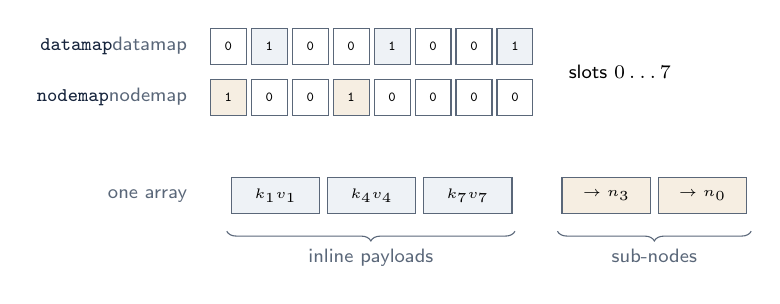
\begin{tikzpicture}[x=1mm,y=1mm]
  % --- the two bitmaps: eight of the thirty-two logical slots shown ---------
  \node[d7label,anchor=east] at (0,0) {\code{datamap}};
  \foreach \i/\b in {0/0,1/1,2/0,3/0,4/1,5/0,6/0,7/1}
    {\node[d7cell, fill={\ifnum\b=1 d7mist\else white\fi}] at (4+\i*5.2,0) {\b};}
  \node[d7label,anchor=east] at (0,-6.5) {\code{nodemap}};
  \foreach \i/\b in {0/1,1/0,2/0,3/1,4/0,5/0,6/0,7/0}
    {\node[d7cell, fill={\ifnum\b=1 d7sun\else white\fi}] at (4+\i*5.2,-6.5) {\b};}
  \node[d7label,anchor=west,font=\sffamily\scriptsize] at (46,-3.2) {slots $0\ldots7$};

  % --- the single backing array --------------------------------------------
  \node[d7label,anchor=east] at (0,-19) {one array};
  \foreach \i/\t in {0/{$k_1v_1$},1/{$k_4v_4$},2/{$k_7v_7$}}
    {\node[d7cell, minimum width=32pt, fill=d7mist] at (10+\i*12.2,-19) {\t};}
  \foreach \i/\t in {0/{$\to n_3$},1/{$\to n_0$}}
    {\node[d7cell, minimum width=32pt, fill=d7sun] at (52+\i*12.2,-19) {\t};}

  \draw[decorate,decoration={brace,mirror,amplitude=3.5pt},d7slate,thin]
    (3.8,-23.5) -- (40.4,-23.5)
    node[midway,below=3pt,d7label] {inline payloads};
  \draw[decorate,decoration={brace,mirror,amplitude=3.5pt},d7slate,thin]
    (45.8,-23.5) -- (70.4,-23.5)
    node[midway,below=3pt,d7label] {sub-nodes};
\end{tikzpicture}
\caption{A CHAMP node. Two bitmaps classify each of the 32 logical slots as
empty, inline payload, or sub-node. The payloads live contiguously at the front
of one array and the sub-node references at the back, so iteration over entries
never has to step past pointers.}
\label{fig:champnode}
\end{figure}

The immediate win is layout. Iteration touches payload runs contiguously instead
of interleaving pointers and payloads, and a lookup that lands on a data slot
reads the entry directly rather than dereferencing a leaf object. The deeper win
is the second change.

\subsection{Canonical deletion topology}

In a plain HAMT, deletion leaves scar tissue.\index{CHAMP!canonical deletion} A sub-node that shrinks to a single
entry stays a sub-node, so the tree's shape encodes its update history: two maps
with identical contents can have different skeletons depending on what was
inserted and removed along the way.

CHAMP normalizes on the way out. When a sub-node shrinks to a single payload, it
is collapsed into its parent's data region; when a wrapper node ends up holding
nothing but a single child, the wrapper is removed (Figure~\ref{fig:champdelete}).
Bitmap topology is therefore determined by the hashes that remain, not by the
order in which they arrived.

\begin{figure}[htbp]
\centering
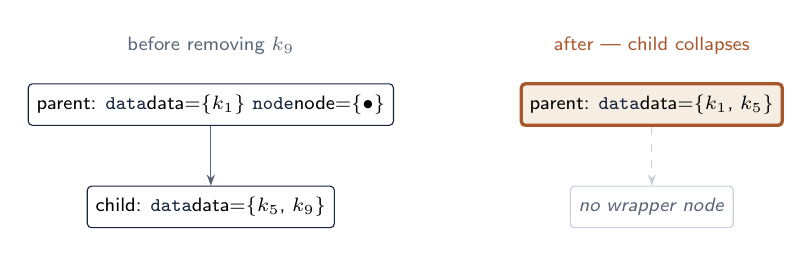
\begin{tikzpicture}[x=1cm,y=1cm]
  \begin{scope}
    \node[d7label] at (1.1,0.75) {before removing $k_9$};
    \node[d7node] (p) at (1.1,0) {parent: \code{data}=\{$k_1$\} \code{node}=\{$\bullet$\}};
    \node[d7node] (c) at (1.1,-1.3) {child: \code{data}=\{$k_5$, $k_9$\}};
    \draw[d7edge] (p) -- (c);
  \end{scope}
  \begin{scope}[xshift=5.6cm]
    \node[d7label,text=d7copper] at (1.1,0.75) {after --- child collapses};
    \node[d7newnode] (p2) at (1.1,0) {parent: \code{data}=\{$k_1$, $k_5$\}};
    \node[d7ghost] (c2) at (1.1,-1.3) {\emph{no wrapper node}};
    \draw[d7edge,draw=d7rule,dashed] (p2) -- (c2);
  \end{scope}
\end{tikzpicture}
\caption{Canonical deletion. A sub-node that would be left holding one payload is
promoted into its parent, so shape depends on contents rather than on history.}
\label{fig:champdelete}
\end{figure}

That canonicalization is what makes the interesting operations possible.

\section{Equality and diff without a lookup pass}

If two maps with equal contents have the same skeleton, then comparing them does
not require looking every key of one up in the other. You can walk both trees in
lockstep, aligning logical bitmap slots, and compare structure directly.
Better: when two versions share ancestry --- which they will, constantly, in a
persistent library --- entire subtrees are \emph{reference-identical}, and a
reference comparison prunes them without touching a single key.\index{reference pruning}

\begin{contractbox}[Structural equality and diff]
Where the implementation has a positive witness that both operands retain one
hash-policy identity, \code{MapEquals} and \code{Diff} traverse aligned logical
slots using stored hashes and prune every reference-identical descendant. Work
then tracks the visited non-shared regions plus the reported differences.
Independently created but compatible policies fall back to lookup-based
comparison, because their coherent hash states may differ.
\end{contractbox}

\begin{caveatbox}[Identical topology is not reference identity]
Two maps built independently --- same entries, same policy, different
allocations --- share nothing. Comparing them is an honest \bigoh{n+m}
traversal, and CHAMP by itself does \emph{not} guarantee work proportional to
logical divergence. The benchmark suite deliberately separates
``shared ancestry, one change'' from ``independent histories, equal contents'',
because those two cost profiles are different and a single number would hide it.

Collision buckets add their own asymmetry. Their internal order is insertion
order, so equality has to match keys as an unordered set, costing up to
\bigoh{c^2} comparisons for a bucket of size $c$. Equal maps may also retain
different concrete key objects, because ``first representative wins'' is
per-history.
\end{caveatbox}

Structural algebra --- union, intersection, difference over two same-type maps or
sets --- uses the same machinery: align slots, prune shared descendants, and
build the result bottom-up.

\section{Collisions}

Two keys whose \emph{entire} 32-bit hash is equal cannot be separated by any
number of levels.\index{collision bucket} CHAMP handles this with an immutable collision bucket: a small
array of entries that share a hash, searched linearly under the equality policy.
This is strictly better than the alternative of extending the trie past the hash
--- there is nothing left to extend it with --- and it degrades gracefully,
because a pathological hash function turns the map into an association list
rather than into an infinite loop.

Unary bitmap chains are a related and often-misunderstood shape. Even under
canonical deletion, a node can legitimately have exactly one child: two keys
whose hashes agree on the first several five-bit groups must be separated deeper
down, and the intervening nodes have nothing else to hold. Canonical here means
\emph{canonical topology given the hashes present}, not ``no node ever has one
child''.

\section{Single-descent factories}

Two operations recur so often in real code that all nine ports expose them
directly rather than making callers compose lookup with update:

\begin{lstlisting}[language={[Sharp]C}]
var withThree = map.GetOrAdd(
    3,
    key => $"value-{key}",
    out string threeValue);

var counted = PersistentHashMap<string, int>.Empty.AddOrUpdate(
    "requests",
    _ => 1,                                 // absent: seed
    (_, current) => checked(current + 1),   // present: update
    out int requestCount);
\end{lstlisting}

Both hash once and descend once.\index{single-descent factories} That is the point: the naive composition
(\code{TryGetValue} then \code{SetItem}) hashes twice and walks the trie twice.
The contract around them is tight, and worth stating in full because it is easy
to get subtly wrong.

\begin{contractbox}[One descent, one factory, no retry]
Delegates are validated \emph{before} hashing. Exactly one factory is selected
and invoked exactly once; \code{GetOrAdd} invokes none on a hit. There is no
retry loop --- unlike a mutable concurrent map, a persistent update has no
competing writer to lose a race to. An update factory receives the caller's
lookup key and the stored value, while the map retains the originally stored key
object. If the produced value compares equal to the stored one, the source map
and the stored value object are both retained. Any factory or comparer exception
leaves the source unchanged and publishes nothing.
\end{contractbox}

\section{Sets, and what changes}

\code{PersistentHashSet} is the same trie with payloads that carry no value. Its
distinctive surface is set algebra and the six set relations --- subset, proper
subset, superset, proper superset, overlap, and set equality --- all of which
preserve the receiver's policy and normalize the argument under it first.

Set algebra benefits from the same reference pruning as map equality: unioning a
set with a descendant of itself skips every shared subtrie. Unioning two
unrelated sets does not, and the API notes say so.

\section{Nine ports, one representation}

Every port ships canonical split-bitmap CHAMP nodes, collision buckets,
persistent path copying, retained hash policies, and stored representatives.
Where they differ is in the optimization tier layered on top:

\begin{d7table}{0.15}
\toprule
\thead{Port} & \thead{Notes beyond the shared representation} \\
\midrule
C\#      & The reference implementation, and the only one with the owner-token
transient kernel (Chapter~\ref{ch:lifecycle}). Lockstep reference-pruned
\code{MapEquals}, bitmap-aligned structural \code{Diff}. \\
Kotlin   & Same split bitmaps and canonical promotion; exact-policy
\code{mapEquals} and typed \code{diff} traverse logical slots in lockstep using
stored hashes. \\
Rust     & Safe \code{Arc} nodes, \code{\#![forbid(unsafe\_code)]}. Both path
copying and \code{BulkBuilder} freezing produce canonical nodes. Independently
created hasher policies keep semantic lookup fallback. \\
Haskell  & Strict split data/node maps, inline \code{(hash,key,value)} runs,
typed \code{MapDifference} values, and indirection-aware pointer pruning.
\code{validStructure} checks the CHAMP invariants. \\
C\texttt{++} & Header-first C\texttt{++}20, move-only bulk builder, compact
inline payload vectors. Independently created stateful hash policies retain
semantic equality/diff. \\
C        & C17, split maps, inline type-erased payloads, flexible-array child
runs, retain/release policy balance, allocation-failure rollback. Diff is
visitor-based so it does not impose an allocator on callers. \\
TypeScript & Canonical CHAMP with reusable public bulk builders; retains the
structural reference-pruning checkpoint. \\
Python   & Canonical CHAMP with the same public semantics, but deliberately
performs semantic lookup-based equality and diff (with exact-policy fast paths)
rather than claiming the lockstep descendant-pruning optimization. \\
OCaml    & Immutable 32-way CHAMP with the same public semantics;
descendant-pruning is implementation-specific and not claimed. \\
\bottomrule
\end{d7table}

\begin{asidebox}[Why enumeration order is a tested non-promise]
It would be easy, and wrong, to let consumers depend on the current trie order.
Durable7 has tests whose entire purpose is to stop that: they assert that
independently built equal maps may enumerate differently, and they exist so that
a future representation change --- a size-tiered small layout, say --- cannot
break downstream code that quietly assumed otherwise. The one place a hash trie
\emph{does} promise an order is Ctrie snapshot conversion
(Chapter~\ref{ch:ctrie}), which fixes canonical data-run-before-node-run order
precisely so that snapshot-to-persistent conversion preserves the captured
sequence.
\end{asidebox}

\chapter{Companions of the Trie}
\label{ch:derived}

\motto{The cheapest new data structure is two old ones that agree with each
other.}

\noindent
Nine families in this library are built by composing existing substrates rather
than by introducing a new core tree.\index{composition-first families} That is a deliberate rule, not an accident
of laziness: a new core is a new set of invariants, a new validator, a new
adversarial test suite, and nine new implementations. A composition inherits all
of that from its parts, and the only genuinely new obligation is keeping the
parts consistent with each other.

\begin{contractbox}[The composite rule]
A composite publishes \emph{all} of its constituent indexes together or
publishes nothing. Counts agree across indexes; no entry exists in only one of
them. Policy-bearing composites retain independent key/value, left/right, or
equality/ordering policies as appropriate, and every mutation preserves retained
versions and returns the receiver for documented logical no-ops.
\end{contractbox}

\section{Persistent hash bag}

\begin{specimen}[Specimen --- \code{PersistentHashBag}]
\index{PersistentHashBag@\texttt{PersistentHashBag}}%
\spec{Purpose}{Unordered multiset: one representative and one positive multiplicity per equality class.}
\spec{Built from}{One CHAMP map from representative to count.}
\spec{Counts}{Distinct-class count and expanded total count are separate values. No ambiguous single ``count'' is exposed.}
\spec{Algebra}{Maximum union, minimum intersection, saturated difference, checked additive sum.}
\spec{Ports}{All nine.}
\end{specimen}

The bag stores multiplicities in $1 \dots 2^{31}-1$ per class --- never zero,
because a zero-multiplicity class is an absent class.\index{multiset} The expanded total is
carried in a wider checked integer, and the choice of type is a small tour of the
nine runtimes: C\# uses a checked \code{long}, TypeScript a \code{bigint},
Python an unbounded \code{int}, OCaml a checked native \code{int}, and the native
ports their corresponding bounded wide integer.

Bag algebra is where the receiver-policy rule earns its keep. A
reference-different argument comparer is normalized eagerly under the receiver's
policy \emph{before} any operation-specific shortcut, and collapsed argument
multiplicities are checked for overflow and use the first representative
observed in that argument version's trie order. Expanded enumeration repeats each
representative contiguously; distinct-item and entry views enumerate one class
each, in the usual stable-but-unspecified order.

\section{Persistent bidirectional map}

\begin{specimen}[Specimen --- \code{PersistentBiMap}]
\index{PersistentBiMap@\texttt{PersistentBiMap}}%
\spec{Purpose}{A strict bijection: each key class and each value class appears at most once.}
\spec{Built from}{A forward CHAMP $K \to V$ and an inverse CHAMP $V \to K$, with independently retained policies.}
\spec{Inverse}{\bigoh{1} in pair count; enumerates nothing.}
\spec{Storage}{Approximately two map entries per logical pair --- stated plainly rather than hidden.}
\spec{Ports}{All nine.}
\end{specimen}

The bimap is the clearest illustration of the composite rule, because its
consistency obligation is symmetric and total: both maps have the same count,
every forward entry has exactly one equivalent inverse entry, and every inverse
entry has exactly one forward entry.\index{bijection} There is no operation that can be halfway
done.

The interesting decisions are in the update semantics.

\begin{itemize}
\item \textbf{Strict add rejects both ways.} Adding a pair whose key class is
occupied fails; so does adding one whose value class is occupied --- even when
the complete pair is equivalent to one already present. The key domain is
checked first, so a result-bearing API reports key conflict before value
conflict. (C\# deliberately keeps its established boolean \code{TryAdd} shape
rather than growing a richer result.)
\item \textbf{Set is not force-put.} Setting adds a missing free pair; treats a
policy-equivalent value update as a no-op that retains both representatives;
replaces a present key's value \emph{only} when the new value class is free; and
never displaces another key. There is no displacing mode, deliberately.
\item \textbf{Replacement goes the long way round.} It removes and reinserts both
directions rather than using the ordinary map's value-equality shortcut, because
that shortcut consults a different policy than the one that governs the inverse
domain.
\item \textbf{Double inversion is free and exact.} C\#, Kotlin, TypeScript, and
Python cache reciprocal facade objects, so \code{map.Inverse.Inverse} is the
original object. The value-semantic ports (C, C\texttt{++}, Haskell, Rust)
guarantee the analogue: double inversion shares the original two immutable roots.
\end{itemize}

The family intentionally exposes no algebra, no builder, no transient, and no
force-put. Each of those would need a bijection-preserving story, and none has a
consumer asking for it.

\section{Set-valued multimap and relation}

\begin{specimen}[Specimen --- \code{PersistentHashMultimap} and \code{PersistentRelation}]
\index{PersistentHashMultimap@\texttt{PersistentHashMultimap}}\index{PersistentRelation@\texttt{PersistentRelation}}%
\spec{Purpose}{One key to many values (multimap); many-to-many with cheap inverse traversal (relation).}
\spec{Built from}{Multimap: CHAMP map from key to non-empty CHAMP set. Relation: two multimaps, forward and reverse.}
\spec{Counts}{Distinct-key count and checked pair count are separate.}
\spec{Inverse}{\code{Inverse} swaps the relation's two persistent indexes without scanning the pair set.}
\spec{Ports}{All nine.}
\end{specimen}

A multimap stores \emph{only} non-empty value sets: removing the last pair for a
key removes the key.\index{multimap} That single invariant is what makes ``does this key have
any values'' a membership test rather than a set-emptiness test, and it is why
duplicate pair insertion and removal of an absent pair are identity no-ops.

The relation adds the reverse index, so asking ``which lefts point at this
right'' is a lookup rather than a scan. Adding or removing a pair updates both
directions atomically; on failure, both indexes and every retained version remain
mutually consistent.

\section{Map patch}

\begin{specimen}[Specimen --- \code{PersistentMapPatch}]
\index{PersistentMapPatch@\texttt{PersistentMapPatch}}%
\spec{Purpose}{A first-class, invertible, composable description of a change to a map.}
\spec{Semantics}{Distinguishes absence from every present value, including null-like ones.}
\spec{Apply}{Validates \emph{all} before-states before applying \emph{any} edit; preserves the source map on conflict.}
\spec{Invert}{Swaps before- and after-states.}
\spec{Compose}{Only through equal intermediate states.}
\spec{Ports}{All nine.}
\end{specimen}

The patch is the library's answer to ``I want to describe a change, inspect it,
send it somewhere, and maybe undo it''.\index{map patch} Its preflight discipline is the whole
design: a patch either applies completely or does not apply at all, and it will
refuse rather than apply half of itself to a map whose before-state has drifted.
The absence-versus-null distinction matters here more than almost anywhere else,
because ``set this key to null'' and ``delete this key'' are different patches
that a sloppier encoding would conflate.

\section{Directed graph}

\begin{specimen}[Specimen --- \code{PersistentDirectedGraph}]
\index{PersistentDirectedGraph@\texttt{PersistentDirectedGraph}}%
\spec{Purpose}{Explicit vertices and unique directed edges with forward and reverse adjacency.}
\spec{Built from}{A vertex set plus two adjacency multimaps.}
\spec{Vertices}{Stored explicitly, so an isolated vertex is a real vertex. Adding an edge adds any missing endpoints.}
\spec{Removal}{Removing a vertex removes every incident edge.}
\spec{Ports}{All nine.}
\end{specimen}

Storing vertices separately from edges is the design decision worth noticing.\index{directed graph}
An edge-list-only graph cannot represent an isolated vertex, which means it
cannot represent ``I have declared this node but not yet connected it'' --- a
state that occurs constantly in dependency graphs and build systems.

\section{Indexed map}

\begin{specimen}[Specimen --- \code{PersistentIndexedMap}]
\index{PersistentIndexedMap@\texttt{PersistentIndexedMap}}%
\spec{Purpose}{A primary map with one automatically maintained non-unique secondary index.}
\spec{Built from}{The primary CHAMP map plus a secondary multimap keyed by a selector result.}
\spec{Invariant}{Exactly one secondary pair per primary key; changing a row's selector class moves its membership atomically.}
\spec{Ports}{All nine.}
\end{specimen}

This is the ``find all users in this city'' structure.\index{secondary index} The selector is applied on
insertion, and the composite's job is to keep the derived index honest across
every edit --- including the awkward one, where updating a row changes which
secondary bucket it belongs to.

\section{Persistent chunked bit set}

\begin{specimen}[Specimen --- \code{PersistentChunkedBitSet}]
\index{PersistentChunkedBitSet@\texttt{PersistentChunkedBitSet}}%
\spec{Purpose}{A sparse set of non-negative 32-bit integers with population rank and select.}
\spec{Core}{64-bit words at the leaves of a measured tree, with a popcount sum measure.}
\spec{Membership}{\bigoh{\log c} for $c$ represented chunks.}
\spec{Rank/select}{Inclusive rank and zero-based select by measured descent.}
\spec{Algebra}{Word-wise merge over sparse streams --- never a scan to the largest index.}
\spec{Ports}{All nine.}
\end{specimen}

The chunked bit set is filed with the trie companions because it plays the same
role --- a set --- but its representation belongs to the sequence world: 64-bit
words at the leaves of a measured tree whose measure is the population count of
its subtree.\index{population count} That measure is what turns \code{Rank} and \code{Select} into
descents rather than scans, and it is a small, satisfying demonstration of how
much the measure framework (Chapter~\ref{ch:measures}) buys.

Zero words are never stored, so storage is proportional to represented chunks
rather than to the largest bit index, and set algebra walks two sparse word
streams rather than iterating a dense range.

\begin{caveatbox}[Which set do you actually want?]
Three families in this library can represent ``a set of integers'', and they are
good at different things. \code{PersistentHashSet} is the general answer with no
ordering. \code{PersistentIntSet} (Chapter~\ref{ch:patricia}) gives ascending
signed order and \emph{structural} merge. \code{PersistentChunkedBitSet} gives
rank and select, and wins hardest when the integers are dense within clusters
and the workload is set algebra. Reach for the third only when rank/select or
word-wise algebra is the reason you are here.
\end{caveatbox}

\chapter{Patricia: When the Key Is Its Own Hash}
\label{ch:patricia}

\motto{A hash trie hashes the key. If the key is already a number, that step is
pure ceremony.}

\begin{specimen}[Specimen --- Patricia integer maps and sets]
\index{Patricia trie!maps and sets}\index{PersistentIntMap@\texttt{PersistentIntMap}}\index{PersistentIntSet@\texttt{PersistentIntSet}}%
\spec{Purpose}{Persistent maps and sets over signed 32- or 64-bit integer keys, with ascending key order and structural merge.}
\spec{Core}{Big-endian path-compressed binary trie: each internal node stores a common prefix and the single bit on which its two subtrees differ.}
\spec{Point ops}{\bigoh{\min(n, W)} for key width $W$ --- in practice a few node hops.}
\spec{Algebra}{Prefix-aligned union, intersection, difference, with combining-function overloads. Work follows visited non-shared prefix regions; \bigoh{n+m} worst case.}
\spec{Order}{Ascending \emph{signed} order, via a sign-bit transform.}
\spec{Ports}{All nine, at both widths: \code{PersistentIntMap}/\code{Set} and \code{PersistentLongMap}/\code{Set} and their local spellings.}
\end{specimen}

\noindent
The hash trie is a fine general answer, and integer keys are the case where it
is least differentiated: hashing an \code{int} to route it through a trie is a
detour, because the key already \emph{is} a well-distributed bit string. Okasaki
and Gill's 1998 paper on mergeable integer maps supplies the structure that
takes the shortcut, and Haskell's \code{Data.IntMap} has been the proof of its
practicality for two decades.

\section{Path compression and the branching bit}

A binary trie over the bits of an integer key would be $W$ levels deep and
mostly empty. Patricia collapses the empty stretches: each internal node stores
the prefix its subtree shares, together with the single bit position at which
its two children diverge.\index{Patricia trie!path compression} Descent is then a prefix test and a bit test ---
no comparisons, no rebalancing, and no rotations, ever.

\begin{figure}[htbp]
\centering
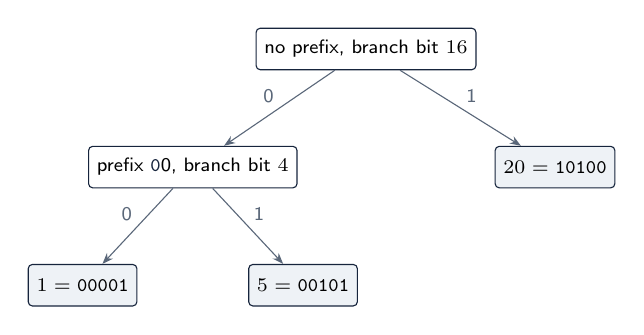
\begin{tikzpicture}[x=1mm,y=1mm]
  \node[d7node] (r)  at (0,0)      {no prefix, branch bit $16$};
  \node[d7node] (l)  at (-22,-15)  {prefix \code{0}, branch bit $4$};
  \node[d7leafnode] (k20) at (24,-15) {$20 = \mathtt{10100}$};
  \node[d7leafnode] (k1)  at (-36,-30) {$1 = \mathtt{00001}$};
  \node[d7leafnode] (k5)  at (-8,-30)  {$5 = \mathtt{00101}$};
  \draw[d7edge] (r) -- node[d7label,above left=-2pt] {0} (l);
  \draw[d7edge] (r) -- node[d7label,above right=-2pt] {1} (k20);
  \draw[d7edge] (l) -- node[d7label,above left=-2pt] {0} (k1);
  \draw[d7edge] (l) -- node[d7label,above right=-2pt] {1} (k5);
\end{tikzpicture}
\caption{A Patricia trie holding $\{1, 5, 20\}$. Keys 1 and 5 agree on every bit
above position 4, so the intervening levels are compressed away and the node
records only the prefix and the branching bit.}
\label{fig:patricia}
\end{figure}

Two pleasant properties fall out immediately. There are no collision buckets,
because distinct keys are distinct bit strings --- the structure is strictly
simpler than the hash trie. And enumeration is in unsigned key order for free,
since the trie is ordered by construction.

\begin{contractbox}[Signed order, by transform]
Raw trie order is unsigned, which puts $-1$ after $2^{31}-1$. Every port applies
a sign-bit transform so that public enumeration is in ascending \emph{signed}
order, and every port ships both an explicit 32-bit and an explicit 64-bit
surface rather than a platform-sized one. Python holds arbitrary-precision
integers at runtime but validates and normalizes keys to the named fixed-width
domain at the public boundary; Haskell exposes \code{Int32}/\code{Int64} aliases
so the width contract does not depend on a platform \code{Int}.
\end{contractbox}

\section{The reason it exists: structural merge}

Point operations are not the interesting part. The differentiator --- the thing
the hash trie genuinely cannot match --- is \term{structural merge}.\index{structural merge}

Union, intersection, and difference align compressed prefixes and descend both
tries together. Where the two prefixes are disjoint, the answer is known without
looking inside either subtree. Where the two subtrees are reference-equal, the
answer is one of them, and the recursion short-circuits. Work is proportional to
the visited non-shared prefix regions plus the materialized result, and a no-op
merge preserves reference identity outright.

That is a categorically different cost profile from merging two hash maps, which
must enumerate one and look up each key in the other. Merge-heavy workloads ---
version-set algebra, sparse indices, identifier-set reconciliation, permission
masks --- stop paying a per-key hash-and-descend and start paying only for
where the two operands actually differ.

\begin{lstlisting}[language={[Sharp]C}]
var baseline = PersistentIntMap<string>.CreateRange(
    new[] { KeyValuePair.Create(-1, "old"), KeyValuePair.Create(10, "ten") });
var delta = PersistentIntMap<string>.CreateRange(
    new[] { KeyValuePair.Create(-1, "new"), KeyValuePair.Create(20, "twenty") });

var merged   = baseline.Union(delta);                    // right-biased
var combined = baseline.Union(delta,
                   (key, left, right) => $"{key}:{left}+{right}");

foreach (var key in merged.Keys)
    Console.WriteLine(key);   // -1, 10, 20 -- ascending signed order
\end{lstlisting}

The combining-function overloads are what make structural merge \emph{useful}
rather than merely fast. Without them, a union has to pick a side and discard
information; with them, a merge can reconcile. The vocabulary is deliberately
modeled on \code{Data.IntMap}'s \code{unionWith}/\code{intersectionWith},
because that is the shape that has proven itself in practice.

\begin{caveatbox}[Sharing lowers the constant, not the bound]
Retained sharing reduces the number of visited regions; it does not define a
separate asymptotic class. The honest worst case remains \bigoh{n+m}, and two
independently constructed tries with identical contents will be walked in full.
As always in this library, the good case is documented as a good case rather
than promoted to a promise.
\end{caveatbox}

\chapter{Ctrie: Snapshots Without Stopping the World}
\label{ch:ctrie}

\motto{A mutable map you can photograph in constant time.}

\begin{specimen}[Specimen --- \code{ConcurrentHashTrie}]
\index{ConcurrentHashTrie@\texttt{ConcurrentHashTrie}}%
\spec{Purpose}{A lock-free \emph{mutable} concurrent hash map whose \code{Snapshot()} is \bigoh{1} and yields an immutable view.}
\spec{Core}{Bitmap C-nodes, singleton leaves, equal-hash collision nodes, and tomb nodes, with generation-stamped indirection nodes.}
\spec{Mechanism}{Node-local GCAS for safe indirection replacement; root/main RDCSS for the snapshot transition; lazy generation renewal on later writes; tomb promotion on deletion.}
\spec{Snapshot order}{Canonical CHAMP order --- data run before node run at every level --- so conversion preserves the captured sequence exactly.}
\spec{Ports}{Full lock-free protocol: C\# and Kotlin/JVM. Synchronous or lock-coordinated snapshot facades: OCaml, TypeScript, Python. Deliberately absent elsewhere.}
\end{specimen}

\noindent
Every other structure in this book is immutable. This one is not, and it earns
its place by solving a problem the immutable structures create.

If your workload is a hot shared cache --- hundreds of thousands of writes a
second from many threads --- a persistent map is the wrong tool, because every
write allocates a path and every writer contends on publishing a new root. But
if that same cache periodically has to hand a \emph{consistent view} to a
reporting thread, a checkpointer, or a serializer, then a plain concurrent hash
map is also the wrong tool, because taking a consistent view means locking
everybody out or copying everything.

Prokopec, Bronson, Bagwell, and Odersky's concurrent trie (PPoPP 2012) sits
exactly in that gap: mutable-map throughput with \bigoh{1} snapshots.

\section{How a constant-time snapshot is possible}

The trick is generation stamping.\index{Ctrie!generation stamping} Every indirection node carries the generation
in which it was created. \code{Snapshot()} does not copy anything; it atomically
installs a new root with a bumped generation. From that moment, any writer that
wants to modify a node belonging to an older generation must first
\emph{renew} it --- copy it into the current generation --- before writing.
Readers holding the old root keep seeing old-generation nodes, which nobody will
ever mutate again.

The subtlety, and the reason this algorithm is famous, is that ``atomically
install a new root'' has to compose with ``atomically replace a node'' without
losing a writer in between. Two mechanisms cooperate:

\begin{description}
\item[GCAS] --- generation-compare-and-set --- makes an indirection node's
replacement safe by publishing a descriptor that readers help complete.\index{GCAS} A reader
that finds a node mid-transition finishes the transition rather than waiting for
it.
\item[RDCSS] --- restricted double-compare single-swap --- makes the root/main
transition atomic with respect to the main-node observation, so a writer cannot
slip between ``I read the main node'' and ``the root was replaced''.\index{RDCSS} The C\#
implementation gives GCAS priority in that transition specifically to close
that window.
\end{description}

Deletion adds a third concern. Removing entries from a deep trie would otherwise
leave a skeleton of empty interior nodes that future traversals still have to
walk. The Ctrie contracts these paths by promoting \term{tomb} nodes --- empty
or singleton markers --- up through their parents, so the structure does not
accumulate scar tissue.\index{tomb node}

\section{Crossing back into the persistent world}

A snapshot is only useful if you can hand it to code that expects an immutable
collection. Conversion is explicit and \bigoh{n}, and its contract is unusually
specific:

\begin{contractbox}[Snapshot conversion preserves the captured sequence]
Snapshot enumeration follows canonical CHAMP ordering: at each bitmap level,
singleton and data entries precede multi-entry child runs; frozen empty tombs
are skipped; frozen singleton tombs are promoted logically into the data run;
and equal-hash collision buckets retain their local order. Explicit
snapshot-to-\code{PersistentHashMap} conversion then preserves that exact
sequence, the exact policy object, stored key and value representatives,
present-null semantics, and isolation from every later live write.
\end{contractbox}

This is the one place in the library where a hash structure commits to an
enumeration order, and the reason is precisely that conversion must be
\emph{exact} rather than merely correct.

\section{Why only two ports have the real thing}

\begin{caveatbox}[The reclamation problem]
Lock-free node replacement is easy to write and hard to free. A thread may be
holding a pointer into a node you have just unlinked, and nothing in the
algorithm tells you when the last such thread is done.

On the CLR and the JVM the garbage collector solves this for free, which is why
C\# and Kotlin ship the complete protocol. In C and C\texttt{++} it would need
epoch-based reclamation or hazard pointers --- a separate project with its own
correctness burden. Rust's \code{Arc} does not help either: sharing an
immutable graph is not the same problem as atomically swapping child pointers,
and a safe design would mean an \code{ArcSwap} or epoch dependency and a new
core. Haskell has a collector but no use for an imperative GCAS algorithm behind
a pure API; \code{STM} or an atomic root wrapper would be a different structure
wearing the same name.

The parity economics therefore cap the lock-free tier at two managed ports, and
the porting guide says so out loud rather than leaving a hole in a matrix.
\end{caveatbox}

OCaml, TypeScript, and Python ship something honest but different: a facade with
the same consumer-level vocabulary --- a mutable map, \bigoh{1} immutable
snapshots --- implemented by serializing operations (an \code{RLock} in Python, a
mutex in OCaml, isolate-locality in TypeScript) and swapping immutable CHAMP
roots. The names preserve the \emph{use case}. They do not claim GCAS, RDCSS,
generation renewal, tomb cleanup, or a lock-free progress guarantee, and their
API notes say so in the first paragraph.

\chapter{Builders, Sessions, and the Frozen Tier}
\label{ch:lifecycle}

\motto{Immutability is a promise about what others can observe, not a vow of
celibacy toward your own unpublished nodes.}

\noindent
Building a million-entry persistent map one \code{SetItem} at a time allocates a
million paths, and only the last one survives. Everyone who has built a
persistent collection library has arrived at the same conclusion: there must be
a way to mutate structure that nobody can see yet.

Durable7 keeps \emph{five} distinct concepts here, and refuses to blur them,
because each has a different lifecycle and a different set of promises
(Figure~\ref{fig:lifecycle}).

\begin{figure}[htbp]
\centering
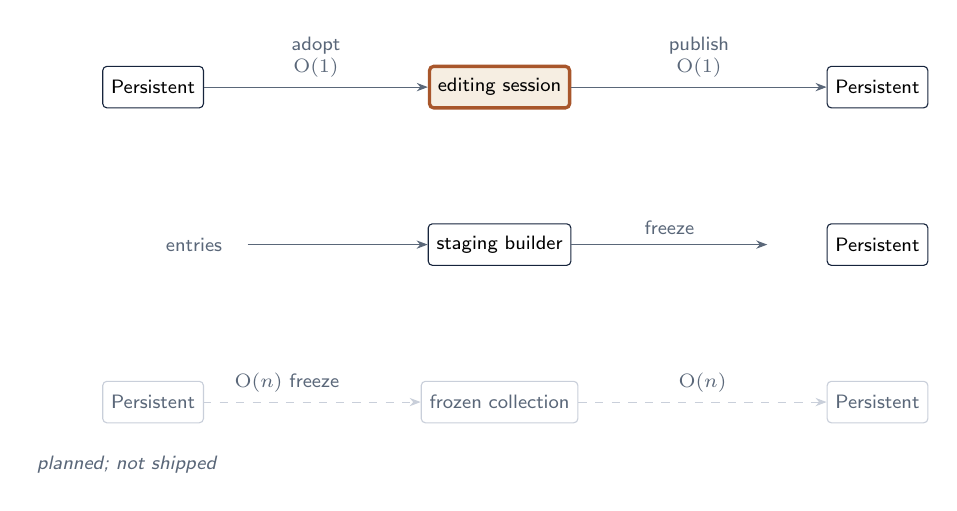
\begin{tikzpicture}[x=1mm,y=1mm]
  \node[d7node] (p1) at (0,0)   {Persistent};
  \node[d7newnode] (s) at (44,0) {editing session};
  \node[d7node] (p2) at (92,0)  {Persistent};
  \draw[d7edge] (p1) -- node[d7label,above,align=center] {adopt\\\bigoh{1}} (s);
  \draw[d7edge] (s) -- node[d7label,above,align=center] {publish\\\bigoh{1}} (p2);

  \node[d7node] (b) at (44,-20) {staging builder};
  \node[d7label,anchor=east] at (10,-20) {entries};
  \draw[d7edge] (12,-20) -- (b);
  \draw[d7edge] (b) -- node[d7label,above] {freeze} (78,-20);
  \node[d7node] (p3) at (92,-20) {Persistent};

  \node[d7ghost] (f) at (44,-40) {frozen collection};
  \node[d7ghost] (p4) at (92,-40) {Persistent};
  \draw[d7edge,dashed,draw=d7rule] (0,-40) -- node[d7label,above] {\bigoh{n} freeze} (f);
  \draw[d7edge,dashed,draw=d7rule] (f) -- node[d7label,above] {\bigoh{n}} (p4);
  \node[d7ghost] at (0,-40) {Persistent};
  \node[d7label,anchor=west,text=d7slate] at (-16,-48) {\emph{planned; not shipped}};
\end{tikzpicture}
\caption{Five distinct lifecycles, kept deliberately separate. The session is
one-way and consumed by publication; the staging builder is reusable and
produces detached snapshots; the frozen tier remains an evidence-gated
proposal.}
\label{fig:lifecycle}
\end{figure}

\section{Construction-only bulk builders}

A bulk builder mutates unpublished leaf, collision, and bitmap nodes in place
during a single construction pass, avoiding a path copy between successive
input entries.\index{bulk builder} It is narrower than an editing session and its contract says so.

\begin{contractbox}[Bulk builder]
Nodes under construction are unpublished and mutated in place. Duplicate
assignment retains the \emph{first} stored key representative, keeps an earlier
equal value representative, and otherwise installs the last distinct value.
Freezing produces a \emph{detached} immutable trie --- later builder mutation
cannot affect an earlier snapshot --- and a reusable freeze leaves the builder
active. Map and set bulk factories use the builder internally; ordinary updates
on an existing persistent collection continue to use structural-sharing path
copies.
\end{contractbox}

C\# uses one internally; C\texttt{++}, Rust, TypeScript, and Python expose the
facility publicly. Rust additionally offers a consuming freeze that moves owned
nodes rather than sharing them. OCaml's reusable staging builder preserves the
detached-freeze semantics and the representative rules but performs persistent
path copying internally, and explicitly does not claim the unpublished
mutable-node construction bound.

\section{The one-way editing session}

A session is the answer to ``I have an existing map and I want to make eighty
changes to it''.\index{editing session} It adopts a persistent root in \bigoh{1}, accepts edits under
single ownership, and publishes once.

\begin{contractbox}[One-way lifecycle]
Adoption and successful publication perform \bigoh{1} trie work and do not
traverse the graph. Sessions preserve the exact equality/hash policy, stored
representatives, unchanged-version trie order, retained source isolation, and
receiver-policy set-relation semantics.

Publication is \emph{one-way}: it consumes the logical session, and the language
either rejects later access dynamically or makes it unavailable through
ownership. A session is unsynchronized and has one logical owner, even where the
language permits explicit handle aliases or moves.

Logical no-ops preserve the current root and do not invalidate a version-bound
view. A clean adopted session therefore republishes the exact source instance.
A failed edit never installs a partial successor.
\end{contractbox}

\subsection{One optimized kernel, eight semantic siblings}

This is the sharpest example in the library of the reference-versus-checkpoint
distinction, and it is worth being precise about.

C\# implements the \term{owner-token transient}: edits mutate only nodes and
arrays proven to be owned by the active edit token, and path-copy anything
shared or sealed.\index{owner-token transient} \code{Persist()} seals the token, publishes without traversing
the graph, and invalidates the mutable object along with every view and
enumerator obtained from it. A clean \code{source.ToTransient().Persist()}
returns the exact source object, including after logical no-op edits.

The other eight ports implement the same \emph{observable lifecycle} over
ordinary persistent path copying. Each changed point edit computes a normal
path-copied successor and replaces the session's current value. They preserve
policy identity, stored representatives, exact clean/no-op root identity,
retained sources, and failure atomicity --- and they make \emph{no}
transient-throughput or allocation-win claim. That is stated in their API notes,
not discovered in a profiler.

\begin{d7table}{0.13}
\toprule
\thead{Port} & \thead{Lifecycle and failure shape} \\
\midrule
C           & Explicit clone/destroy handles over one reference-counted state.
Clones are lifecycle \emph{aliases}: one successful publication consumes them
all. Operations report a consumed or modified status; failed edits and relation
queries preserve session and output atomicity. \\
C\texttt{++} & Sessions are movable but not copyable and publish only through
\code{std::move(session).persist()}. Generation-bound iterators reject changed
or consumed sessions. A throwing custom policy move terminally invalidates the
source (and, for assignment, the destination), and publication after such a move
carries no retry guarantee --- nothrow-movable policies avoid both boundaries. \\
Haskell     & Sessions live in \code{IO} and are consumed by
\code{persistMap}/\code{persistSet}. Candidate construction precedes a masked
commit, so neither synchronous nor asynchronous failure can partially install an
edit. \\
Kotlin      & Consumption is enforced at runtime. Acquired views capture the
current snapshot and session version, survive logical no-ops, and fail after
content changes. Callback failure leaves the session unchanged and retryable. \\
OCaml       & The session retains one persistent root, replaces it with path-copy
successors, and dynamically rejects access after publication. The reusable bulk
builder is a separate facility. \\
Rust        & Publication is \code{into\_persistent(self)}, so the type system
prevents use-after-publication. \code{into\_transient} moves a source;
\code{to\_transient} shares its root. \\
TypeScript  & One-way publication enforced at runtime inside one JavaScript
isolate; no cross-worker progress claim. \\
Python      & Consumes on publication and invalidates iterators after content
changes or publication. \\
\bottomrule
\end{d7table}

\section{The frozen tier, and why it has not shipped}

The third lifecycle --- \bigoh{n} conversion to a read-optimized layout with no
update-shaped API --- is designed, prototyped, and deliberately unshipped.\index{frozen collection tier}

Its intended contract is already written down: separate \code{FrozenHashMap} and
\code{FrozenHashSet} types, one offline-built general hash layout for every count
and key type, preserved comparer identity and stored representatives, preserved
source traversal sequence, no library-controlled allocation on point lookup, and
enumeration that is stable for an unchanged instance but otherwise unspecified
--- never insertion, sorted, canonical, or serialization order. Freezing an
already-frozen value is identity; converting back is visibly \bigoh{n}.

What is missing is evidence. The track is staged: a faithful packed-index signal
first, fixed layouts compared only once a credible read-heavy regime appears, and
a public type authorized only behind lookup, enumeration, memory, and realistic
construction break-even numbers. The benchmark-local candidates already cover the
low-risk half --- rebuilding canonical CHAMP from a packed source-order entry
sequence through the existing bulk builder, with an untimed verifier locking
comparer identity, traversal sequence, representative rules, null and collision
behavior, and round-trip reconstruction.

\begin{asidebox}[Deliberate non-adaptivity]
Tiny flat layouts, string prefix and length dispatch, integer-key routing,
binary-fuse and ribbon filters, Eytzinger and PGM sorted layouts, and
count-derived representation selectors are all postponed --- not rejected,
postponed. The stated reason is methodological: the value of the \emph{temporal}
lifecycle (transient, persistent, frozen) is being isolated before it is
combined with size or key specialization, so that a later benchmark can tell
which of the two produced a gain. Benchmarks may contain tiny and string
datasets; that is a workload, not permission to select a representation.
\end{asidebox}

% ===========================================================================
%  PART III -- SEQUENCES
% ===========================================================================
\part{Sequences}
\label{part:sequences}

\chapter{Finger Trees}
\label{ch:fingertree}

\motto{A tree that keeps its hands in its pockets: whatever else is deep, both
ends are always within reach.}

\begin{specimen}[Specimen --- \code{FingerTreeDeque} and \code{FingerTree}]
\index{FingerTreeDeque@\texttt{FingerTreeDeque}}\index{FingerTree@\texttt{FingerTree}}%
\spec{Purpose}{A persistent indexed sequence with cheap endpoints and cheap concatenation (\code{FingerTreeDeque}), and a general monoid-measured tree used directly and as the engine beneath a dozen facades (\code{FingerTree}).}
\spec{Core}{Hinze and Paterson's 2-3 finger tree: digits at each end, a recursively nested spine of nodes in the middle.}
\spec{Endpoints}{\bigoh{1} amortized push and pop at either end.}
\spec{Concat}{\bigoh{\log \min(n,m)} --- proportional to the \emph{smaller} operand.}
\spec{Index / split}{\bigoh{\log d}, where $d$ is the distance from the nearer end. The measured U-shape.}
\spec{Ports}{All nine: \code{FingerTreeDeque}/\code{PersistentDeque}/\code{persistent\_deque}/\code{Deque}, plus the measured tree under each language's local name.}
\end{specimen}

\noindent
Most balanced trees treat all positions alike.\index{finger tree} A finger tree does not: it keeps
a small unbalanced ``digit'' of one to four elements at each end and pushes the
balanced structure into the middle, where a recursively nested spine holds
\emph{nodes} of two or three elements, which themselves hold nodes, and so on
(Figure~\ref{fig:fingertree}).\index{digit}

\begin{figure}[htbp]
\centering
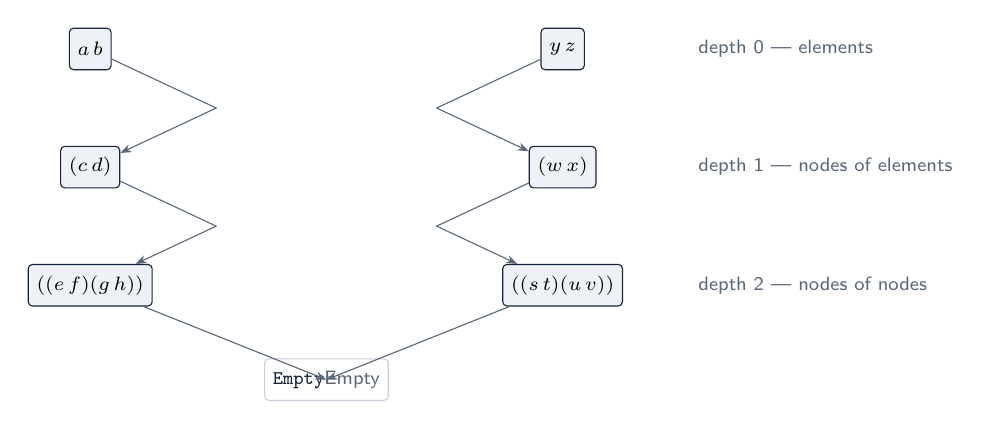
\begin{tikzpicture}[x=1mm,y=1mm]
  \foreach \y/\lft/\rgt/\lbl in {%
     0/{$a$\,$b$}/{$y$\,$z$}/{depth 0 --- elements},
   -15/{$(c\,d)$}/{$(w\,x)$}/{depth 1 --- nodes of elements},
   -30/{$((e\,f)(g\,h))$}/{$((s\,t)(u\,v))$}/{depth 2 --- nodes of nodes}}
  {
    \node[d7leafnode] (L\y) at (-30,\y) {\lft};
    \node[d7leafnode] (R\y) at ( 30,\y) {\rgt};
    \node[d7label,anchor=west] at (46,\y) {\lbl};
  }
  \draw[d7edge] (L0)   -- (-14,-7.5) -- (L-15);
  \draw[d7edge] (R0)   -- ( 14,-7.5) -- (R-15);
  \draw[d7edge] (L-15) -- (-14,-22.5) -- (L-30);
  \draw[d7edge] (R-15) -- ( 14,-22.5) -- (R-30);
  \node[d7ghost] at (0,-42) {\code{Empty}};
  \draw[d7edge] (L-30) -- (0,-42);
  \draw[d7edge] (R-30) -- (0,-42);
\end{tikzpicture}
\caption{The finger-tree shape. Both ends sit at depth zero and stay there; only
the middle gets deeper. This is why endpoint operations are constant-amortized
while indexing costs a logarithm of the distance to the nearer end.}
\label{fig:fingertree}
\end{figure}

That asymmetry is the whole design. Pushing onto an end usually just grows a
digit, which is \bigoh{1}; occasionally a digit overflows and a node is pushed
one level down, and the amortized analysis --- with memoized lazy suspensions
spreading the debt across later forces --- keeps the average constant.
Concatenation is proportional to the logarithm of the \emph{smaller} operand,
because the two spines only have to be zipped together as deep as the shorter
one goes. Indexing costs a logarithm of the distance to the nearer end, so both
\code{seq[0]} and \code{seq[n-1]} are nearly free while the middle is
logarithmic --- the ``measured U-shape'' the API notes refer to.

\section{The deque}

\code{FingerTreeDeque<T>} is the tuned sequence facade. It exposes endpoint
operations, concatenation, splitting, positional edits, and range operations.

\begin{lstlisting}[language={[Sharp]C}]
var deque    = FingerTreeDeque<int>.Create(1, 2, 3);
var extended = deque.AddFirst(0).AddLast(4);

var first    = extended.PopFirst();
var rest     = first.Rest;                 // [1, 2, 3, 4]

var split    = rest.SplitAt(2);
var joined   = split.Left.Concat(split.Right);
var replaced = joined.SetItem(1, 20);      // [1, 20, 3, 4]
\end{lstlisting}

It also carries a small set of helpers for sequences the caller \emph{knows} to
be sorted --- \code{SortedLowerBound}, \code{SortedUpperBound},
\code{InsertSorted}, \code{SplitAtSortedEqualRange}. These assume sortedness
rather than maintaining it, which is exactly the right split of
responsibilities: if sortedness is a long-lived invariant, the sorted
collections of Chapter~\ref{ch:sorted} maintain it for you; if it is a passing
property of a sequence you happen to have, these helpers exploit it without
committing you to a different type.

\section{The measured tree}

The general \code{FingerTree<TElement, TMeasure, TMeasureOps>} is the deque's
more powerful sibling and the engine underneath sorted bags, sets and maps,
priority queues, interval trees, ropes, and the chunked bit set. Every node
caches the monoidal summary of its subtree, and the tree can be split at the
first position where a predicate over the running prefix measure flips from
false to true.

That single operation --- \term{split by measure} --- is startlingly general.
Measure by element count and you get positional indexing. Measure by maximum key
and you get sorted lookup. Measure by minimum priority and you get a priority
queue. Measure by maximum interval endpoint and you get interval search. Measure
by newline count and you get a text editor's line index. Chapter~\ref{ch:measures}
is entirely about this idea.

\begin{contractbox}[Finger-tree core obligations]
Empty, singleton, endpoint, concatenation, split, index, insert, remove, and
range operations preserve immutable snapshot semantics. Measure policies supply
an identity, an element measure, and an associative combine. Split and locate
depend on a documented predicate boundary over prefix measures, and any new
measure or predicate helper must document the ordering assumptions it needs.
Product and sum measures preserve component order and component-specific
predicate mapping. Lazy middle publication and cached measures must never expose
partially initialized data to a reader.
\end{contractbox}

\begin{caveatbox}[This was once a checkpoint boundary]
Until August 2026 this box named a real gap: five ports built their sorted
collections, priority queues, and interval trees over a measured AVL or another
balanced tree rather than a lazy-spine finger tree, and their API notes recorded
the weaker asymptotic claim rather than inferring the stronger one. All five have
since been rebuilt, so every port now carries the lazy Hinze--Paterson core and
the bounds above hold in all nine. Chapter~\ref{ch:laziness} is the account of
why the difference mattered, how it was found, and what a strict language must
build by hand to close it.
\end{caveatbox}

\chapter{Measures: Monoids as Connective Tissue}
\label{ch:measures}

\motto{Give a tree an associative summary and it will answer questions you never
built it to answer.}

\noindent
This chapter has no data structure of its own. It describes the abstraction that
makes a third of the library possible, and it is the single best return on
conceptual investment in this book.

\section{The idea}

A \term{measure} is a monoid --- a type with an identity element and an
associative binary combine --- plus a function from an element to a value of
that type.\index{measure} Cache the measure of every subtree on its root node, and two things
become cheap:

\begin{enumerate}
\item \textbf{Aggregate queries.} The measure of the whole sequence is the
measure at the root, read in \bigoh{1}. The measure of a range is a logarithmic
boundary computation.
\item \textbf{Measure-guided descent.} Walk from the root, accumulating the
running prefix measure. At each node, ask whether the prefix \emph{including}
the left subtree satisfies a predicate. If yes, descend left; if no, add the left
measure to the accumulator and descend right. You have located the first
position where the predicate flips, in \bigoh{\log n}, without visiting the
elements you skipped.
\end{enumerate}

Associativity is what makes step 2 sound --- it lets the accumulated prefix be
computed in any grouping.\index{monoid!associativity} Commutativity is \emph{not} required, and the library
is scrupulous about this: ordered measures are combined strictly left to right,
and several tests exist specifically to prove that a non-commutative measure
behaves.

\begin{contractbox}[What a measure policy must supply]
An identity value; an element measure; an associative combine. Nothing more.
Predicates used for split and locate must be monotone over the running prefix
measure --- false, then true, with no oscillation --- because descent is a binary
search and an oscillating predicate makes the answer meaningless. Collections
cannot repair an unlawful policy, and such policies are outside the logical
contract.
\end{contractbox}

\section{The measures that ship}

\begin{d7table}{0.24}
\toprule
\thead{Measure} & \thead{What it turns the tree into} \\
\midrule
Size / count & A positionally indexed sequence: split at ``prefix count $>$ $i$''
gives element $i$. \\
Sum & A prefix-sum sequence; range sums by boundary subtraction where the
element type allows it, or by ordered range measure where it does not. \\
Maximum & An ordered structure: split at ``prefix max $\geq$ $k$'' is a sorted
lower bound. Underpins sorted sets, bags, and maps. \\
Minimum & A priority queue: the root measure is the front priority, and descent
locates it. \\
Order statistic (count + last key) & Sorted collections that also support rank
and select. \\
Interval (count, last low, max high) & An interval tree: a subtree whose maximum
high endpoint is below the probe cannot contain an overlap, so it is pruned. \\
Newline & A text rope: line count in the measure turns line/column navigation
into a descent. \\
Popcount & The chunked bit set: inclusive rank and zero-based select by measured
descent over 64-bit words. \\
Product / pair & Two measures carried together, preserving component order and
mapping predicates to the right component. This is how ``sorted \emph{and}
indexable'' works. \\
\bottomrule
\end{d7table}

\section{How the nine ports spell it}

The abstraction is the same everywhere; only its encoding is local. C\#,
C\texttt{++}, Kotlin, and Python expose typed measure abstractions (with
comparison and predicate abstractions where their surfaces need them); C exposes
equivalent policy callbacks with context pointers; Haskell uses an ordinary
type class and plain functions \code{v -> Bool} as predicates, because in
Haskell a predicate abstraction would be ceremony. Rust exposes a
\code{MeasurePolicy} trait plus a generous set of ready-made measures ---
\code{SizeMeasure}, \code{SumMeasure}, \code{MaxMeasure}, \code{MinMeasure},
\code{KeyMeasure}, \code{ProductMeasure}, \code{OrderStatisticMeasure}, and the
combined \code{SizeAndSum}/\code{SizeAndMax}/\code{SizeAndMin} forms.

\begin{asidebox}[Where measures paid off unexpectedly]
The chunked bit set was originally imagined as a HAMT-backed structure, and it
half-failed the library's own test for whether a composition is load-bearing.
The recommended prototype instead put \code{ulong} chunks at the leaves of a
measured tree with a popcount sum measure --- and got membership, inclusive
rank, select, and reference-short-circuiting set algebra out of machinery that
already existed. That is the measure framework doing what it is for: a new
public capability with no new core.
\end{asidebox}

\chapter{RRB Vectors}
\label{ch:rrb}

\motto{The persistent vector everybody means when they say ``persistent
vector''.}

\begin{specimen}[Specimen --- \code{RrbVector}]
\index{RrbVector@\texttt{RrbVector}}%
\spec{Purpose}{A persistent sequence with \emph{uniform} random access --- no U-shape --- plus logarithmic concatenation and splitting.}
\spec{Core}{Relaxed radix-balanced tree: 32-way branches, 32-element leaves. Regular branches are radix-indexed with pure bit arithmetic and carry no size table; only branches touched by concatenation carry cumulative sizes.}
\spec{Index}{\bigoh{\log_{32} n} with a small constant, uniform across positions.}
\spec{Endpoints}{\bigoh{\log_{32} n} --- there is deliberately no persistent tail buffer.}
\spec{Concat}{\bigoh{\log_{32}(n+m)} boundary-spine merge.}
\spec{Builder}{Append-only, freezes full leaves safely and caches immutable snapshots.}
\spec{Ports}{All nine.}
\end{specimen}

\noindent
Bagwell and Rompf's relaxed radix-balanced tree (2011, with the practical
transient treatment in Stucki et al., ICFP 2015) is the structure behind Scala's
persistent vector, Clojure's \code{core.rrb-vector}, C\texttt{++} \code{immer},
and Rust \code{im}. Its central trick is to be a radix trie \emph{most} of the
time.

\section{Regular and relaxed branches}

In a plain radix trie of branching factor 32, finding index $i$ is pure bit
arithmetic: take five bits of $i$ per level and you are there.\index{radix trie} No size tables, no
comparisons. That works only if every node is full, which stops being true the
moment you concatenate two vectors.

RRB's answer is to allow both kinds of node (Figure~\ref{fig:rrb}). A
\term{regular} branch is full and radix-indexable; it stores no size table at
all.\index{RRB vector!regular branch} A \term{relaxed} branch carries a small array of cumulative sizes and is
searched rather than computed.\index{RRB vector!relaxed branch} Concatenation introduces relaxed branches only
along the seam; everything away from the seam stays regular and stays fast.

\begin{figure}[htbp]
\centering
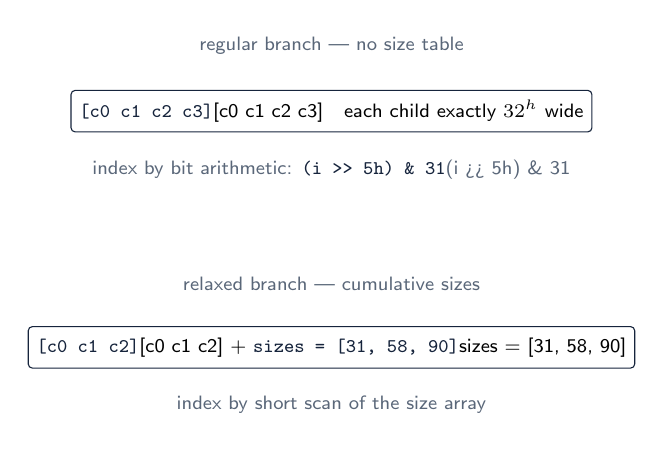
\begin{tikzpicture}[x=1mm,y=1mm]
  \node[d7label,anchor=south] at (24,10) {regular branch --- no size table};
  \node[d7node,minimum width=48mm] (reg) at (24,4) {\code{[c0 c1 c2 c3]}\quad each child exactly $32^h$ wide};
  \node[d7label,anchor=north,align=center] at (24,-1)
    % NB: >{}> rather than >> -- T1 makes a guillemet ligature out of the latter.
    {index by bit arithmetic: \code{(i >{}> 5h) \& 31}};

  \node[d7label,anchor=south] at (24,-20) {relaxed branch --- cumulative sizes};
  \node[d7node,minimum width=48mm] (rel) at (24,-26) {\code{[c0 c1 c2]} + \code{sizes = [31, 58, 90]}};
  \node[d7label,anchor=north,align=center] at (24,-31)
    {index by short scan of the size array};
\end{tikzpicture}
\caption{RRB nodes come in two flavors. Only nodes disturbed by concatenation
pay for a size table; the rest keep the radix trie's pure bit-arithmetic
indexing.}
\label{fig:rrb}
\end{figure}

\section{The representation boundary, stated up front}

\begin{caveatbox}[Boundary-spine concatenation, not global redistribution]
All ports deliberately implement \emph{boundary-spine} concatenation: the two
child arrays at the seam are repartitioned, and nothing is promised about
minimum fullness for leaves or branches away from that seam. The full
Stucki-et-al.\ redistribution pass is not performed.

The adversarial density assertions in the test suites are regression gates for
the histories they exercise --- not a validator-certified representation
contract. What the validators \emph{do} certify is a size-derived height cap:
$\lfloor (\text{bit width of the count type} - 1)/5 \rfloor + 1$. The first term
is the greatest minimum height required anywhere in the count domain; the extra
level admits the boundary-only contract's legal ``minimum height $+\,1$'' slack
even in the top count band. That works out to seven for the C\#/Kotlin
\code{Int} count domain and thirteen on 64-bit
\code{size\_t}/\code{Int}/\code{usize} targets. TypeScript and Python apply their
own checked runtime count domains.
\end{caveatbox}

\section{Choosing between three sequences}

The library ships three persistent sequences with overlapping capabilities, and
declines to pretend one of them wins.

\begin{d7tablethree}{0.20}{0.23}
\toprule
\thead{Workload} & \thead{Finger-tree deque} & \thead{Rope \hfill / \hfill RRB vector} \\
\midrule
Endpoint push/pop & \bigoh{1} amortized --- best & \bigoh{\log n}, staged
amortized \bigoh{1} \hfill / \hfill \bigoh{\log_{32} n}, no persistent tail \\
Random index, middle & \bigoh{\log n}, U-shaped & \bigoh{\log n} chunked
\hfill / \hfill \bigoh{\log_{32} n}, small constant --- best \\
Concatenation & \bigoh{\log \min} --- best & \bigoh{\log \min}
\hfill / \hfill \bigoh{\log n} with relaxed nodes \\
Cache density & pointer-heavy & chunked, best for scans \hfill / \hfill 32-way
arrays, good \\
Bulk build & element-wise & chunk-staged builder --- best \hfill / \hfill
builder tier \\
\bottomrule
\end{d7tablethree}

The RRB vector's differentiator is uniform indexing. The shipped persistent value
deliberately has \emph{no} dedicated tail buffer, so endpoint operations remain
logarithmic and the separate append-only builder is the bulk-construction path.
Concatenation is logarithmic but with worse constants than the deque's.

The library's stance is unusually restrained here: it ships the vector, ships
benchmark comparisons against the rope and the platform's own immutable list,
and tells consumers to choose on their measured workload rather than on the
asymptotics. Shipping an implementation does not, by itself, erase the overlap
with two existing sequence families.

\chapter{Ropes and Text}
\label{ch:rope}

\motto{A string that does not mind being edited in the middle.}

\begin{specimen}[Specimen --- \code{Rope}, \code{MeasuredRope}, \code{TextRope}]
\index{Rope@\texttt{Rope}}\index{MeasuredRope@\texttt{MeasuredRope}}\index{TextRope@\texttt{TextRope}}%
\spec{Purpose}{Persistent chunked sequences (\code{Rope}), the same with a custom split/locate measure (\code{MeasuredRope}), and a newline-aware text specialization (\code{TextRope}).}
\spec{Core}{Runs of elements held contiguously in immutable leaf chunks at the leaves of a measured tree.}
\spec{Edits}{\bigoh{\log n} plus bounded chunk work.}
\spec{Concat / split}{\bigoh{\log \min} / \bigoh{\log n}.}
\spec{Scans}{Array speed within a chunk --- the reason to prefer a rope over a pointer-per-element sequence.}
\spec{Ports}{All nine, each with positional, measured, and text cursors.}
\end{specimen}

\noindent
The rope's insight is that the atoms of a sequence do not have to be its
elements.\index{rope} Put a run of elements in one contiguous immutable leaf, and you get
tree behavior for edits with array behavior for scans --- which is exactly the
trade a text editor wants, since editing is local and rendering is sequential.

\section{Three layers, one machine}

\begin{description}
\item[\code{Rope<T>}] is positional. Its measure is element count; indexing,
splitting, insertion, removal, concatenation, and slicing are all defined over
logical element offsets.
\item[\code{MeasuredRope<T, M>}] replaces the count measure with a caller's
monoid, so split and locate can be driven by anything associative. It inherits
the measure-law requirements of Chapter~\ref{ch:measures} wholesale.
\item[\code{TextRope}] is the measured rope specialized to a newline measure,
plus the helpers that make text navigation pleasant: line and column
conversion, line extraction, newline-style handling.\index{text rope}
\end{description}

Because \code{TextRope} is a specialization rather than a separate core, its
line index is not a side table that can drift out of sync --- it is the measure,
maintained by the same code path that maintains everything else.

\begin{caveatbox}[What a text position counts]
This is the least portable thing in the library, and the docs are correspondingly
blunt about it. Text positions count: UTF-16 code units in C\#, Kotlin, and
TypeScript; \code{char}-sized bytes in C and C\texttt{++}; Haskell \code{Char}
elements; Unicode scalar values in OCaml and Rust; Unicode code points in
Python. \emph{None} of them denotes a grapheme cluster index. Line and column
rules are zero-based, and the C port uses LF-only newline recognition.

If you are writing cross-language code that exchanges text offsets, this is the
paragraph that will save you.
\end{caveatbox}

\section{Builders}

Ropes are commonly built from a stream rather than edited into existence, so
every port has a builder that stages chunks and publishes an immutable rope.
The contract that matters is publication isolation: later builder changes cannot
affect a previously produced rope. As with the trie builders, mutation is
confined to nodes nobody can see.

\chapter{The Range-Update Sequence}
\label{ch:range}

\motto{Lazy propagation, but you are allowed to keep the old version.}

\begin{specimen}[Specimen --- \code{RangeUpdateSequence}]
\index{RangeUpdateSequence@\texttt{RangeUpdateSequence}}%
\spec{Purpose}{An immutable indexed sequence that can apply one algebraic transformation to a contiguous range, and query that range's aggregate, without visiting the covered elements.}
\spec{Core}{A separately owned path-copied implicit AVL --- \emph{not} a tagged modification of either finger-tree engine.}
\spec{Whole-sequence update}{\bigoh{1}: one new root.}
\spec{Subrange update / query}{\bigoh{\log n} boundary work.}
\spec{Point edit, split, concat}{\bigoh{\log n}.}
\spec{Policy}{A tag monoid acting lawfully on elements and on cached ordered measures, with an explicit composition direction.}
\spec{Ports}{All nine. OCaml ships an immutable-array checkpoint with the same public algebra and persistence semantics and makes no implicit-AVL lazy-update claim.}
\end{specimen}

\noindent
Competitive programmers know the ephemeral version of this structure as a
segment tree with lazy propagation, and it is one of the great practical
algorithms: ``add 7 to every element between positions 200 and 9{,}000'' in
logarithmic time, by writing a pending instruction on a handful of internal
nodes instead of touching nine thousand elements.\index{lazy propagation}

Making it persistent is harder than it sounds, because the classic
implementation \emph{pushes} pending tags down as it descends --- and pushing is
mutation. In a persistent structure a read must not mutate anything, because
another version is looking at those same nodes.

\section{The invariant that makes it work}

The library resolves this with a carefully chosen convention
(Figure~\ref{fig:rangetag}):

\begin{contractbox}[The node invariant]
A node's stored value and cached measure \emph{already include} that node's own
pending tag.\index{pending tag} Its children do \emph{not}.

Structural descent and rotations push a pending tag down before rearranging
nodes. Read-only indexing, range measurement, and enumeration instead carry the
inherited tag down the path and compose it after the node's older tag --- never
writing to shared storage.
\end{contractbox}

\begin{figure}[htbp]
\centering
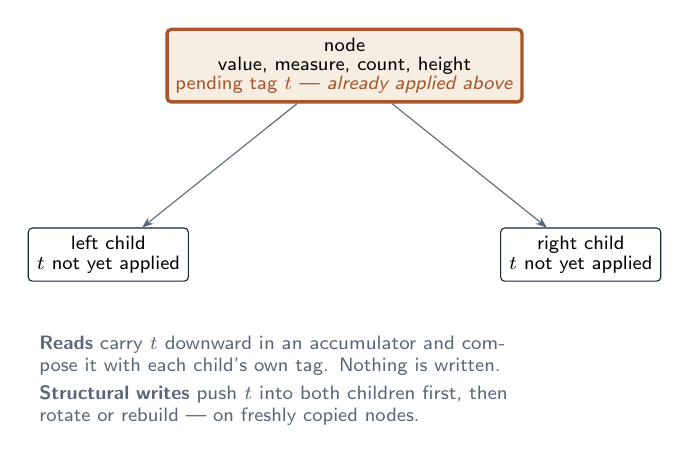
\begin{tikzpicture}[x=1mm,y=1mm]
  \node[d7newnode,align=center] (n) at (0,0)
    {node\\[-1pt]{\scriptsize value, measure, count, height}\\[-1pt]
     {\scriptsize\color{d7copper}pending tag $t$ --- \emph{already applied above}}};
  \node[d7node,align=center] (l) at (-30,-24) {left child\\[-1pt]{\scriptsize $t$ not yet applied}};
  \node[d7node,align=center] (r) at ( 30,-24) {right child\\[-1pt]{\scriptsize $t$ not yet applied}};
  \draw[d7edge] (n) -- (l);
  \draw[d7edge] (n) -- (r);
  \node[d7label,anchor=west,align=left,text width=62mm] at (-40,-40)
    {\textbf{Reads} carry $t$ downward in an accumulator and compose it with each
     child's own tag. Nothing is written.\\[2pt]
     \textbf{Structural writes} push $t$ into both children first, then rotate or
     rebuild --- on freshly copied nodes.};
\end{tikzpicture}
\caption{The pending-tag convention. Because a node's own summary already
reflects its tag, a whole-subtree transformation is a single-node path copy, and
cached measures stay queryable without ever visiting an element.}
\label{fig:rangetag}
\end{figure}

The payoff is direct. Applying a non-identity tag to the entire sequence
allocates exactly one new root --- \bigoh{1}, regardless of length. A proper
subrange decomposes into \bigoh{\log n} maximal covered subtrees plus two
boundary paths, so it is logarithmic. And because a node's cached measure is
already tag-inclusive, range aggregate queries are logarithmic too, with no
element visits at all.

\section{The algebra, and its laws}

The policy --- \code{IRangeUpdateAlgebra<TElement, TMeasure, TTag>} in C\#, with
local spellings elsewhere --- extends the ordinary measure monoid with a tag
monoid and two actions.\index{tag algebra} The single most important detail is the composition
direction, and it is stated everywhere it appears:

\begin{center}
\fbox{\parbox{0.86\linewidth}{\centering\vspace{2pt}
\code{Compose(newer, older)} means: apply \emph{older} first, \emph{newer}
second.\vspace{2pt}}}
\end{center}

The executable law gate covers the following, and a policy that violates them is
outside the collection's logical contract --- the structure cannot repair an
unlawful action and does not pretend to:

\begin{itemize}
\item the measure has an identity and an associative ordered combine;
\item tags have an identity and an associative composition in that direction;
\item the tag action on an element composes in the same order;
\item the tag action on a cached measure composes in the same order \emph{and
receives the represented element count};
\item applying a tag to a singleton measure agrees with measuring the tagged
element;
\item the action distributes over ordered measure combination with the correct
left and right counts --- tested with a non-commutative measure;
\item applying any tag to the empty measure at count zero yields the empty
measure; and
\item every tag that \code{IsIdentity} recognizes --- including a value-distinct
representation of identity --- obeys the full identity equations.
\end{itemize}

\section{In use}

The canonical example is an affine algebra whose tags either assign a value or
add to it, over a sum measure:

\begin{lstlisting}[language={[Sharp]C}]
using Sequence = Durable7.FingerTree.RangeUpdateSequence<
    long, long, AffineTag, AffineSumAlgebra>;

var source   = Sequence.Create([1, 2, 3, 4]);
var added    = source.ApplyRange(1, 2, AffineTag.Add(10));
// [1, 12, 13, 4], Measure == 30

var assigned = added.ApplyRange(2, 2, AffineTag.Assign(7));
// [1, 12, 7, 7], Measure == 27

long middleSum = assigned.MeasureRange(1, 2);   // 19
var (prefix, suffix) = assigned.SplitAt(2);
var reconstructed = prefix.Concat(suffix);

// source is still [1, 2, 3, 4].
\end{lstlisting}

Note what the API deliberately does \emph{not} have: there is no \code{AddRange}
or \code{AssignRange} method on the generic core, because those verbs belong to
a particular tag algebra rather than to the sequence. The core knows about tags;
it does not know what they mean.

\begin{contractbox}[Behavioral obligations]
Retained versions stay immutable and share unaffected interiors. Range
validation precedes tag callbacks; empty ranges preserve the receiver and the
empty measure without invoking the policy at all; recognized identity updates
preserve the receiver. Direct insert, replace, and remove push old tags before
installing new content, so a prior range tag never leaks onto newly inserted
elements. Any policy exception publishes no successor.
\end{contractbox}

\begin{caveatbox}[Enumerator copying]
The concrete enumerator is a mutable struct that is deliberately \emph{not}
safe to copy mid-traversal: copies share traversal state and the stale copy
fails fast once the other advances. Independently created enumerators are fully
independent and safe for concurrent reads. This is the standard trade for a
non-allocating enumerator, and the fail-fast behavior exists so that the
mistake surfaces immediately rather than as silent misreads.
\end{caveatbox}

\chapter{The Reversible Deque}
\label{ch:revdeque}

\motto{Reversal as a fact about how you are looking, not about where things
are.}

\begin{specimen}[Specimen --- \code{ReversibleDeque}]
\index{ReversibleDeque@\texttt{ReversibleDeque}}%
\spec{Purpose}{A persistent sequence for which logical reversal is a primary operation.}
\spec{Core}{Persistent deque storage plus an orientation bit or mirrored root.}
\spec{Reverse}{\bigoh{1} --- a new view over shared storage, not a materialized sequence.}
\spec{Everything else}{Endpoint operations, indexing, splitting, concatenation, traversal, and materialization all observe the current logical orientation.}
\spec{Ports}{All nine.}
\end{specimen}

\noindent
This is the smallest structure in the book and it makes a point worth more than
its size: a great many ``operations'' are really changes of perspective, and
a persistent library is in an unusually good position to represent them as such.\index{orientation}

\begin{lstlisting}[language={[Sharp]C}]
var deque    = ReversibleDeque<int>.Create(1, 2, 3);
var reversed = deque.Reverse();

var first    = reversed[0];        // 3
var restored = reversed.Reverse(); // shares storage with deque
\end{lstlisting}

\begin{contractbox}[Orientation obligations]
Reversal returns a new value and preserves the original. Every operation ---
endpoints, indexing, splitting, concatenation, traversal, materialization ---
observes the logical orientation. Mixed-orientation concatenation must not
silently reinterpret one operand in physical order. An \bigoh{1} reversal claim
belongs only where the implementation genuinely uses an orientation bit,
mirrored root, or equivalent view rather than materializing a new sequence.
\end{contractbox}

That last clause is the interesting one. It would be easy for a port to
implement \code{Reverse} by building a reversed copy, keep every observable
behavior identical, and quietly break the one promise anybody chose the type
for. The repository maintains a dedicated complexity audit for exactly this
family, and it is the required reading before touching any orientation-aware
implementation.

\chapter{DABA Lite: The Deliberate Outlier}
\label{ch:daba}

\motto{Not persistent, not sorry.}

\begin{specimen}[Specimen --- \code{DabaLite}]
\index{DabaLite@\texttt{DabaLite}}%
\spec{Purpose}{Maintain the aggregate of a FIFO sliding window under any associative monoid --- no commutativity, no inverse required.}
\spec{Core}{The De-Amortized Banker's Aggregator (Lite), over a linked queue of 64-slot chunks with six ordered cursors.}
\spec{Callback ceilings}{Insert invokes \code{Combine} at most three times; evict at most twice; query at most once; an empty query, none. Unconditional.}
\spec{Operations}{Worst-case \bigoh{1} structural work, given \bigoh{1} monoid callbacks.}
\spec{Mutability}{\textbf{Mutable and unsynchronized.} This is the one collection in the book that is not persistent.}
\spec{Ports}{All nine.}
\end{specimen}

\noindent
Every other structure in this book preserves its old versions. This one
overwrites them on purpose, and it belongs here anyway for two reasons: it is the
measure framework's first consumer outside the trees, and it answers a question
the trees answer worse.

The question is: what is the sum --- or max, or concatenation, or any associative
combination --- of the last $k$ items in a stream, updated as items arrive and
depart? A finger tree answers it in \bigoh{\log n}. Tangwongsan, Hirzel, and
Schneider's aggregator (DEBS 2017, with the Lite representation in the 2021
journal article) removes the logarithm entirely for this deliberately mutable
special case.

\section{Six cursors and a bounded fixup}

The window is a queue of partial aggregates, overlaid with six cursors that
always satisfy $F \leq L \leq R \leq A \leq B \leq E$
(Figure~\ref{fig:daba}).\index{sliding window} Between them they delimit the front, left, right,
accumulator, and back regions; two extra fields carry the products that do not
live in queue slots.

\begin{figure}[htbp]
\centering
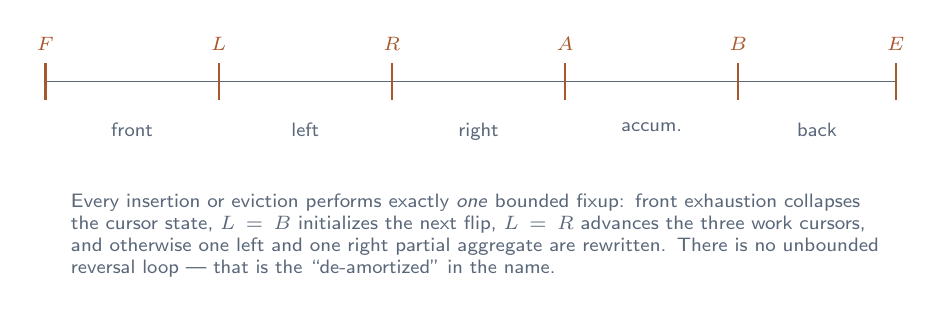
\begin{tikzpicture}[x=1mm,y=1mm]
  \draw[d7slate,thin] (0,0) -- (108,0);
  \foreach \x/\n in {0/F, 22/L, 44/R, 66/A, 88/B, 108/E}
    {\draw[d7copper,thick] (\x,-2.4) -- (\x,2.4);
     \node[d7label,above=1pt,text=d7copper] at (\x,2.4) {$\n$};}
  \foreach \a/\b/\t in {0/22/{front}, 22/44/{left}, 44/66/{right},
                        66/88/{accum.}, 88/108/{back}}
    {\node[d7label,below=3pt] at ({(\a+\b)/2},-3) {\t};}
  \node[d7label,anchor=north west,align=left,text width=104mm] at (2,-13)
    {Every insertion or eviction performs exactly \emph{one} bounded fixup:
     front exhaustion collapses the cursor state, $L = B$ initializes the next
     flip, $L = R$ advances the three work cursors, and otherwise one left and
     one right partial aggregate are rewritten. There is no unbounded reversal
     loop --- that is the ``de-amortized'' in the name.};
\end{tikzpicture}
\caption{The DABA Lite cursor state. The schedule is what makes the operation
bounds worst-case rather than amortized.}
\label{fig:daba}
\end{figure}

The invocation ceilings --- three, two, one --- are unconditional and tested
directly by counting callbacks. What is \emph{not} unconditional is the wall
clock: the complete operations are worst-case \bigoh{1} only when the monoid's
\code{Combine} and identity are themselves \bigoh{1}. The library states the
ceiling and the condition separately, which is the honest way to do it.

\section{The parts that differ by runtime}

\begin{caveatbox}[Clear is not \bigoh{1} everywhere]
On the tracing runtimes --- C\#, Kotlin/JVM, TypeScript, Python --- \code{Clear}
swaps in one fresh empty chunk in \bigoh{1} and invokes \code{Combine} zero
times.

In C, C\texttt{++}, and Rust it is deliberately \bigoh{n + c} for $n$ values
across $c$ chunks, because deterministic destruction has to actually release
$n$ generic owned values. All three break the chain iteratively, neither leaking
nor deferring an unbounded retired representation. Insert, eviction, and query
keep their worst-case \bigoh{1} structural and callback work in every port.

Python is a third case: it clears by replacing the active chain in \bigoh{1},
but unreachable cyclic backing may be reclaimed later by the collector, so it
does not claim the native ports' prompt deterministic destruction.
\end{caveatbox}

Failure behavior is similarly runtime-shaped but semantically uniform: a
throwing monoid callback leaves the published window unchanged for every
mutating operation. C\texttt{++} achieves this by building a private fixup plan
under a nothrow-move value constraint and committing without throwing; Rust
plans candidate aggregates, slot rewrites, and a possible successor chunk before
publication so a panic cannot expose a partial mutation; C stages
callback-produced values in seven fixed aligned temporaries and transfers
ownership by byte move.

\section{What it will not do}

\begin{caveatbox}[No oldest-value access, no enumeration, no synchronization]
The Lite schedule intentionally overwrites raw values with partial aggregates,
so there is no API to read the oldest value or enumerate the window --- the
information is genuinely gone. There is no synchronization either; callers must
not overlap access to one instance without external serialization. And the type
is \emph{ephemeral}: it is a fit for transient streaming state, not a persistent
replacement for a deque.
\end{caveatbox}

\section{Space, and a validator that knows nothing}

The paper's logical accounting is $n + 2$ values: $n$ queue partial aggregates
plus the two aggregate fields. The chunked implementations instead allocate
capacity for $n$ live positions plus 1 to 127 slack slots, and an empty instance
retains one 64-slot block.

\code{ValidateStructure} is deliberately callback-free and content-blind. In
\bigoh{c} time and space for $c$ active chunks it checks links, cursor
reachability and order, the count and distance equations, the DABA region-size
equations, and the chunk/slack bound --- and returns a statistics record with the
count, five region lengths, active block count, allocated capacity, and slack.
It cannot check that the aggregate is \emph{correct}, because the original values
may already have been overwritten; correctness is tested against an external FIFO
model instead. That division of labor is a small model of the whole repository's
approach to validation.

% ===========================================================================
%  PART IV -- ORDER AND PRIORITY
% ===========================================================================
\part{Order and Priority}
\label{part:order}

\chapter{Sorted Collections}
\label{ch:sorted}

\motto{A measured tree with a maximum-key measure is a sorted set. Everything
else is presentation.}

\begin{specimen}[Specimen --- \code{SortedBag}, \code{SortedSet}, \code{SortedDictionary}]
\index{SortedBag@\texttt{SortedBag}}\index{SortedSet@\texttt{SortedSet}}\index{SortedDictionary@\texttt{SortedDictionary}}%
\spec{Purpose}{Immutable comparer-ordered multisets, sets, and key/value maps, with rank and boundary queries.}
\spec{Core}{Order-statistic measures over the measured tree --- typically cached count plus last key --- in the mature ports; an idiomatic ordered storage checkpoint elsewhere.}
\spec{Identity}{\emph{Comparison} defines equality here, not hashing. Two values that compare equal are the same element.}
\spec{Enumeration}{Bag: sorted, with duplicates. Set: sorted, one representative per equivalence class. Map: sorted by key.}
\spec{Builders}{Batched edits published as one immutable snapshot.}
\spec{Ports}{All nine.}
\end{specimen}

\noindent
These are the collections most people reach for first, and in this library they
are facades: put a measure that summarizes ``the largest key in this subtree''
on a measured tree, and splitting at ``prefix maximum $\geq k$'' \emph{is} a
sorted lower bound.\index{sorted collections} Add a count to the measure --- a product measure --- and the
same tree also supports rank and select. The sorted collections are that
observation, dressed for use.

\begin{contractbox}[Sorted-collection obligations]
Comparison policy defines equality. If two values compare equal, the API must
document whether duplicates are counted, rejected, replaced, or merged --- and
each of the three families answers differently, which is the point of having
three.

Sorted bag enumeration includes duplicates in sorted order. Sorted set
enumeration contains one representative per comparison-equivalent value. Sorted
map lookup, rank, and boundary queries use key comparison, never hash equality.
Rank and index APIs must define zero- versus one-based indexing, miss behavior,
and duplicate handling. Builders must document when they stop sharing with
immutable snapshots and when snapshots are published.
\end{contractbox}

\begin{caveatbox}[Comparison equality is not hash equality]
A value can be equal under a comparer and unequal under an equality comparer, or
vice versa, and mixing the two families in one program is a reliable source of
confusion. A case-insensitive comparer makes \code{"Key"} and \code{"key"} the
same element in a \code{SortedSet} and different elements in a
\code{PersistentHashSet} --- unless the hash policy agrees, which it will only
do if someone made it agree. The library keeps the two policy kinds firmly
separate and never derives one from the other.
\end{caveatbox}

\chapter{Canonical Sorted Sets: Zip and Zip-Zip Trees}
\label{ch:canonical}

\motto{For collections compared far more often than they are modified.}

\begin{specimen}[Specimen --- \code{CanonicalSortedSet} and \code{ZipTreeRankPolicy}]
\index{CanonicalSortedSet@\texttt{CanonicalSortedSet}}\index{ZipTreeRankPolicy@\texttt{ZipTreeRankPolicy}}%
\spec{Purpose}{A sorted set whose \emph{shape} is determined by its contents under a retained rank policy, so equal sets converge on equal topology and inequality is usually rejected in \bigoh{1} by a memoized digest.}
\spec{Core}{Zip-zip tree: a randomized-rank binary search tree where insertion and deletion are single root-to-position \term{unzip} and \term{zip} passes --- no rotations.}
\spec{Ranks}{A geometric primary coordinate and a fixed 64-bit secondary coordinate, both derived from HMAC-SHA-256 over the equivalence class.}
\spec{Policy modes}{An unexposed random key, a public reproducibility seed, or a caller-retained secret key.}
\spec{Equality}{Memoized root digest rejects most inequality in \bigoh{1}; shared nodes prune the rest; independently built equal sets still cost \bigoh{n}.}
\spec{Ports}{All nine.}
\end{specimen}

\noindent
Tarjan, Levy, and Timmel's zip trees (2018/2019) reformulate the treap so that
insertion and deletion are single passes: to insert, \term{unzip} the search
path into two spines and hang them off the new node; to delete, \term{zip} the
two child spines back together.\index{zip tree} Expected restructuring is \bigoh{1} and there is
no rotation code at all. Gila, Goodrich, and Tarjan's zip-zip trees (2023) refine
the rank distribution so that expected depth approaches the information-theoretic
optimum.\index{zip-zip tree}

What Durable7 wants from them is not speed. It is \emph{canonicity}.

\section{Shape from contents}

If a node's rank is derived from its key rather than drawn fresh at insertion
time, then under one retained coherent rank policy, the tree's shape is a
function of its contents (Figure~\ref{fig:zip}).\index{rank policy} Insert the same elements in a
different order and you converge on the same topology.

\begin{figure}[htbp]
\centering
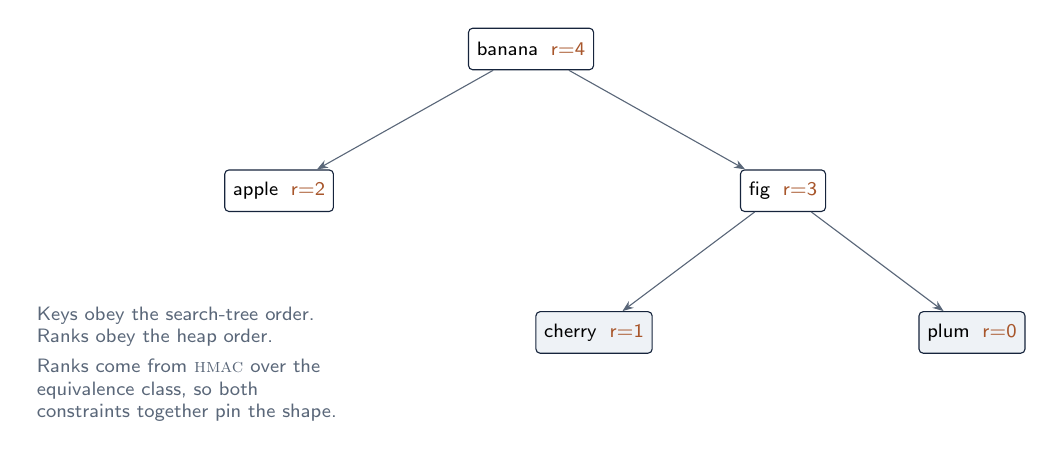
\begin{tikzpicture}[x=1mm,y=1mm]
  \node[d7node] (b) at (0,0)      {$\mathsf{banana}$ \;\textcolor{d7copper}{r$=$4}};
  \node[d7node] (a) at (-32,-18)  {$\mathsf{apple}$ \;\textcolor{d7copper}{r$=$2}};
  \node[d7node] (f) at ( 32,-18)  {$\mathsf{fig}$ \;\textcolor{d7copper}{r$=$3}};
  \node[d7leafnode] (c) at ( 8,-36) {$\mathsf{cherry}$ \;\textcolor{d7copper}{r$=$1}};
  \node[d7leafnode] (p) at ( 56,-36) {$\mathsf{plum}$ \;\textcolor{d7copper}{r$=$0}};
  \draw[d7edge] (b) -- (a); \draw[d7edge] (b) -- (f);
  \draw[d7edge] (f) -- (c); \draw[d7edge] (f) -- (p);
  \node[d7label,anchor=west,text width=52mm,align=left] at (-64,-40)
    {Keys obey the search-tree order.\\
     Ranks obey the heap order.\\[3pt]
     Ranks come from \textsc{hmac} over the\\
     equivalence class, so both\\
     constraints together pin the shape.};
\end{tikzpicture}
\caption{A zip-zip tree. Because ranks are derived rather than drawn, the search
order and the heap order jointly determine the topology for a given content set
under a given policy.}
\label{fig:zip}
\end{figure}

Canonical shape is worth having when a collection is compared far more often
than it is modified: memoization keys, configuration fingerprints, cache
validity stamps. A memoized root digest rejects most inequality in constant
time; shared node identity prunes the equal case; and independently built equal
sets fall back to an honest \bigoh{n} comparison.

\section{Getting ranks right}

The rank source has to be stable, well distributed, and coherent with the
comparer --- and this turns out to be where the design gets interesting.

\begin{contractbox}[Rank policy obligations]
A policy may use an unexposed random key, a public reproducibility seed, or a
caller-retained key. An explicit comparer must \emph{also} supply a rank hash
that is constant on its equivalence classes; duplicate representatives
dynamically check that contract.

Set equality is semantic across policy families, but canonical structural
algebra is gated on policy identity. First-representative retention means
equivalent values can still retain different concrete objects, so this is
\term{policy-canonical} topology --- not a claim of globally unique
representation.
\end{contractbox}

\begin{caveatbox}[What the fixed-width variant does not inherit]
This is a practical fixed-width implementation, not the paper's compact
representation. Its 64-bit secondary coordinate does not inherit the paper's
\bigoh{\log \log n}-metadata theorem, and the 64-bit caller hash (32-bit for the
fallback) can collide before HMAC ever runs. Expected-depth claims therefore
require a well-distributed, stable, equivalence-class-coherent rank source.

A keyed policy resists adaptive rank prediction only while the caller-retained
key stays secret; a public seed buys reproducibility, not adversarial security.
And persistence changes the cost profile: an ephemeral zip tree changes
\bigoh{1} expected pointers, but a persistent update still copies its
search/zip/unzip path --- expected \bigoh{\log n} nodes, \bigoh{n} under
adversarial ranks.
\end{caveatbox}

The implementations take the stack-safety problem seriously, because a fully
colliding rank chain is a legitimate adversarial input: zip and unzip are
explicit-stack rather than recursive, and destruction uses an intrusive
non-allocating worklist so that reclaiming a 16{,}384-node chain neither
recurses nor allocates.

Cryptographic sourcing is likewise concrete rather than hand-waved: CNG on
Windows and OpenSSL elsewhere for C and C\texttt{++}, RustCrypto HMAC/SHA-256
with \code{getrandom} for Rust, \code{crypton} for Haskell, \code{hashlib} and
\code{hmac} for Python. Rust and Python both pin stable rank hashes explicitly
rather than trusting a default hasher, because \code{DefaultHasher} and
randomized \code{str} hashing are exactly the failure this structure cannot
tolerate.

\chapter{Insertion Order as a First-Class Property}
\label{ch:ordered}

\motto{Two collections can hold the same elements and still not be the same
list.}

\begin{specimen}[Specimen --- the neutral Ordered family]
\index{Ordered family (insertion-ordered)}\index{PersistentOrderedSet@\texttt{PersistentOrderedSet}}\index{PersistentOrderedMap@\texttt{PersistentOrderedMap}}\index{PersistentOrderedMultimap@\texttt{PersistentOrderedMultimap}}%
\spec{Purpose}{Sets, maps, and multimaps whose enumeration follows first insertion plus explicit positional operations --- neither hash order nor comparison order.}
\spec{Core}{A persistent hash membership/stamp index composed with a persistent ordered sequence. Deliberately independent of any other family.}
\spec{Identity}{Equality policy decides membership and representatives. It never decides position.}
\spec{Operations}{Explicit movement, positional reads, ranges, reversal, stable one-shot sort, receiver-policy set algebra, all six set relations.}
\spec{Ports}{All nine: \code{PersistentOrderedSet}, \code{PersistentOrderedMap}, \code{PersistentOrderedMultimap}.}
\end{specimen}

\noindent
Insertion order is the order humans expect.\index{insertion order} It is what a configuration file
means, what a UI list means, what a pipeline stage sequence means. Hash order is
an implementation detail and comparison order is somebody else's opinion; if the
program's meaning depends on the sequence in which things were added, that has
to be represented deliberately.

\section{Two indexes, one meaning}

The family composes a hash index --- which answers membership and holds
representatives --- with a persistent ordered sequence, which answers position.
The composite obligation from Chapter~\ref{ch:derived} applies in full: both
indexes publish together or neither does, counts agree, and no entry exists in
only one.

\begin{contractbox}[Ordered-family obligations]
Equality policy defines membership, duplicate collapse, stored representatives,
algebra, and relations; every result retains the exact receiver policy,
including empties.

Construction and duplicate additions retain the \emph{first} representative
\emph{and its position} --- a duplicate add never moves or replaces anything.
Movement is explicit, retains the stored representative, and interprets a
supplied destination as the final result index.

Union appends argument-only classes after receiver order; intersection and
difference retain receiver order; symmetric difference emits receiver-only then
argument-only classes. All algebra and all six relations eagerly enumerate and
normalize the complete argument under the receiver policy \emph{before} applying
any shortcut, so a late enumeration or policy failure is visible rather than
optimized away.

Documented logical no-ops return the receiver; failures publish nothing; private
sparse position labels are not API, and a relabel rebuild leaves retained
versions untouched.
\end{contractbox}

The map adds one rule that is easy to get wrong and important to get right:
setting an existing key changes \emph{only} its payload. It does not replace the
stored key representative and it does not move the entry. Range construction
retains the first key representative and its first position while the last
payload for that class wins. Equality policy controls key identity and never
payload equality or sort order.

The multimap nests the same idea: key groups retain first-insertion order, and
the distinct values within each group retain their own first-insertion order.
Enumeration is grouped, and an empty group is never stored.

\begin{asidebox}[On sparse labels and branching]
Insertion-ordered structures are usually implemented with sparse integer
position labels and midpoint insertion, which occasionally require a wholesale
relabel. That relabel is an \bigoh{n}-at-threshold amortization --- precisely
the kind that Chapter~\ref{ch:persistence} warns does not survive branching.
The library's response is to treat the labels as strictly private, to state the
worst case per produced version rather than the amortized one, and to guarantee
that a relabel rebuild leaves retained versions untouched. The related
general-purpose \code{OrderMaintenanceList} --- the Dietz--Sleator structure that
answers ``does $A$ precede $B$?'' --- remains unbuilt for want of a named
consumer (Appendix~\ref{app:roads}).
\end{asidebox}

\chapter{Priority: Three Structures, Three Reasons}
\label{ch:priority}

\motto{``Give me the smallest one'' has more variations than it looks.}

\noindent
Three families in this library answer priority questions, and they are not
redundant --- each exists because the other two are wrong for a specific need.

\section{The measured priority queue}

\begin{specimen}[Specimen --- \code{PriorityQueue}]
\index{PriorityQueue@\texttt{PriorityQueue}}%
\spec{Purpose}{The general persistent minimum-priority queue.}
\spec{Core}{A minimum-priority measure over the measured tree.}
\spec{Bounds}{Amortized: \bigoh{1} peek, \bigoh{\log n} enqueue and dequeue, \bigoh{\log \min} meld.}
\spec{Ties}{Equal priorities drain in insertion order.}
\spec{Ports}{All nine.}
\end{specimen}

This is the default, and it is a measure facade: cache the minimum priority of
each subtree, and locating the front entry is a descent.\index{priority queue} Melding two queues is
concatenation. It costs nothing conceptually beyond the measure framework, which
is exactly why it is the default.

\begin{lstlisting}[language={[Sharp]C}]
var queue = PriorityQueue<string, int>.Empty
    .Enqueue("slow", 10).Enqueue("fast", 1).Enqueue("normal", 5);

if (queue.TryPeek(out var element, out var priority))
{
    // element == "fast"; priority == 1
}
\end{lstlisting}

\section{The Brodal--Okasaki heap}

\begin{specimen}[Specimen --- \code{BrodalOkasakiHeap}]
\index{BrodalOkasakiHeap@\texttt{BrodalOkasakiHeap}}%
\spec{Purpose}{Worst-case rather than amortized latency for insert, meld, and minimum.}
\spec{Core}{Bootstrapped skew-binomial queues (Brodal and Okasaki, JFP 1996).}
\spec{Bounds}{\bigoh{1} \emph{worst-case} insert, meld, and find-minimum; \bigoh{\log n} worst-case delete-minimum.}
\spec{Meld}{Requires comparer object identity --- even when one operand is empty.}
\spec{Enumeration}{Unspecified structural order. Equal elements have no stable tie order. Delete repeatedly for sorted output.}
\spec{Ports}{All nine.}
\end{specimen}

The measured queue has the same bounds \emph{amortized}.\index{Brodal--Okasaki heap} This heap's entire
reason for existing is the word ``worst-case'': if a latency budget is a hard
requirement rather than an average, an amortization spike is a bug. The
implementation is a direct port of the fused bootstrapped skew-binomial
representation, with comparison-count tests that assert the operation bounds
rather than merely believing them.

\begin{asidebox}[One algorithm, two spellings]
The C and C\texttt{++} \code{skew\_meld} implementations consolidate the child
forest by rank buckets with carry; C\#, Haskell, Kotlin, and Rust spell the
equivalent step as \code{uniquify} followed by \code{unionUnique}. This is an
intentional native implementation-shape difference. Both produce the same valid
ranked-tree multiset, the same minimum, and the same public bounds --- and the
repository records the divergence explicitly so that a future reader does not
mistake it for a porting error.
\end{asidebox}

\begin{caveatbox}[Why not strict Fibonacci or hollow heaps?]
Strict Fibonacci heaps (Brodal, Lagogiannis, and Tarjan, STOC 2012) and hollow
heaps (Hansen, Kaplan, Tarjan, and Zwick, ICALP 2015) achieve optimal
decrease-key bounds through aggressive pointer mutation --- and persistent path
copying destroys exactly the surgery they depend on. They are recorded as
explicit non-goals rather than as omissions.
\end{caveatbox}

\section{The priority search queue}

\begin{specimen}[Specimen --- \code{PrioritySearchQueue}]
\index{PrioritySearchQueue@\texttt{PrioritySearchQueue}}%
\spec{Purpose}{Keyed lookup \emph{and} minimum-priority removal \emph{and} a combined key-range plus priority-threshold query, in one structure.}
\spec{Core}{A persistent AVL ordered by key, each node caching its subtree's minimum-priority winner.}
\spec{Bounds}{\bigoh{1} minimum; \bigoh{\log n} keyed update, removal, and delete-minimum; \bigoh{\log n + v} range query where $v$ counts nodes pruning cannot exclude.}
\spec{Ties}{Priority ties break by key order --- deterministic, not merely stable.}
\spec{Ports}{All nine.}
\end{specimen}

A heap cannot find a key.\index{priority search queue} A map cannot find the minimum. The priority search
queue does both, and adds the query that motivates it: \emph{which entries in
this key range have priority at most $p$?} That is the scheduler question, the
expiry question, and the task-queue question.

\begin{lstlisting}[language={[Sharp]C}]
var jobs = PrioritySearchQueue<string, int, string>.Create(
        StringComparer.Ordinal, Comparer<int>.Default)
    .SetItem("compile", 3, "Build the solution")
    .SetItem("deploy",  8, "Publish artifacts")
    .SetItem("audit",   1, "Check invariants");

var next   = jobs.Minimum;                                  // "audit", 1
var urgent = jobs.EnumerateAtMost("a", "z", maximumPriority: 3);
jobs = jobs.DeleteMinimum(out var removed);
\end{lstlisting}

\begin{asidebox}[A deliberate departure from Hinze]
Hinze's ICFP 2001 priority search queue uses \term{priority-search pennants}: a
loser tree over a weight-balanced search tree, whose threshold-only
\code{at-most} operation has the output-sensitive bound
$\Theta(r(\log n - \log r + 1))$ for $r$ results.

Durable7 deliberately uses a different representation --- a persistent AVL node
carrying its own entry plus a cached subtree winner --- and claims the bounds
that representation actually delivers: \bigoh{\log n} keyed operations,
\bigoh{1} minimum, and \bigoh{\log n + v} for the inclusive key-range and
priority-threshold traversal, where $v \leq n$ is the number of visited nodes
that pruning could not exclude. The worst case is therefore \bigoh{n} for a dense
result, and no pennant-specific output bound is claimed. Choosing a simpler
representation and reporting its real bounds is treated as preferable to
importing a bound the code does not earn.
\end{asidebox}

\chapter{Intervals}
\label{ch:interval}

\motto{Everything that has a beginning and an end wants one of these.}

\begin{specimen}[Specimen --- \code{IntervalTree} and \code{PersistentIntervalMap}]
\index{IntervalTree@\texttt{IntervalTree}}\index{PersistentIntervalMap@\texttt{PersistentIntervalMap}}%
\spec{Purpose}{Ordered collections of intervals with overlap and point-stabbing queries (tree), and the same with one payload attached to each complete interval key (map).}
\spec{Core}{Interval annotations in the measure: typically count, last low endpoint, and maximum high endpoint.}
\spec{Pruning}{A subtree whose maximum high endpoint lies below the probe cannot contain an overlap, so the descent skips it entirely.}
\spec{Map key}{The \emph{complete} \code{(low, high)} pair. Intervals sharing only one endpoint stay distinct.}
\spec{Ports}{All nine.}
\end{specimen}

\noindent
The interval tree is the measure framework's most elegant payoff. Put the
maximum high endpoint of a subtree in its measure, and a stabbing query becomes
a descent that prunes any subtree which \emph{provably} cannot contain a match ---
without looking at a single interval inside it.\index{interval tree}

\begin{contractbox}[Interval obligations]
Interval construction must define whether empty or inverted intervals are
rejected, normalized, or accepted. Endpoint comparison policy defines ordering,
equality, overlap, and containment. Query APIs must document endpoint
inclusivity and behavior when several overlaps exist. Removal must state whether
it removes one match, all matches, or a comparison-equivalent representative.
\end{contractbox}

The interval \emph{map} adds a payload and, with it, a second index: an exact
lookup index keyed by the complete interval pair, alongside the augmented search
index. The composite rule applies --- both contain the same intervals, payloads,
and count. Replacing a payload preserves the stored interval representative and
neither duplicates nor moves the key; stabbing and overlap queries return entries
in the local deterministic interval order.

% ===========================================================================
%  PART V -- RESEARCH-DERIVED COLLECTIONS
% ===========================================================================
\part{Narrow Questions}

\chapter{Ancestry as a Sequence}
\label{ch:ancestry}

\motto{The sequence is not stored anywhere in particular. It is two boundaries
on a path that already exists.}

\noindent
Seven of this library's collections did not arrive the way the others did.\index{research-derived collections}
The finger tree, the hash trie, the RRB vector and their relatives are
implementations of published structures: the paper came first, the library
followed. These seven began instead as scoped design studies --- each one a
normative proposal written before any code, asking whether a narrow question
that the general structures answer badly could be answered well by giving
something up.

The proposals share a discipline that is worth naming before any of the
structures are described, because it is the reason their claims can be trusted.

\begin{contractbox}[How a research-derived collection is argued]
\emph{It answers a narrow question.} Every proposal states the question, names
the general structure that answers it worse, and says plainly when the general
structure is the right choice anyway.

\emph{It declares its non-goals.} Concatenation of unrelated histories, point
replacement, middle editing, confluent merge --- whatever the design cannot do
is listed, and no comparison table is ever allowed to count an omitted
operation as a fast one.

\emph{It separates two complexity statements and never conflates them.} One is
the bound the shipped code delivers. The other is the bound the same reduction
would deliver over a stronger component that exists in the literature but is not
implemented here. Both appear; they are never merged into a single optimistic
number.

\emph{Its novelty claim is scoped.} ``Not found in a targeted literature
search'' is written as exactly that, and never as priority.
\end{contractbox}

The seven are: \code{AncestralSliceQueue} and \code{BilateralAncestralDeque},
the subjects of this chapter; \code{ContextualRankSequence} (Chapter~\ref{ch:contextual}), which ranks and
selects events whose occurrence is not a property of an element but of the
finite-state context to its left; \code{PersistentDeltaMap} (Chapter~\ref{ch:checkpoint}), an ordered map that
maintains its own exact checkpoint-relative change set and emits it in time
proportional to the number of changes rather than the size of the map;
\code{PersistentRunDeltaVector}, in the same chapter, which does the same for a
fixed-length vector
and reports \emph{maximal dirty runs} rather than dirty positions;
\code{PersistentMonotoneActionHeap} (Chapter~\ref{ch:actions}), a meldable min-heap
that applies a monotone
transformation to every entry in \bigoh{1} and still melds in \bigoh{1}
afterwards, even when the transformation has no inverse; and
\code{PersistentAncestralConnectionForest} (Chapter~\ref{ch:connectivity}), an
insertion-only connectivity
structure that can name the earliest version on a lineage at which two vertices
became connected, for the price of one ordinary connectivity query.

All seven were prototyped in C\#, lived for a time in \code{*.Experimental}
namespaces, and were then promoted and ported to all nine languages --- the
TypeScript port last, in August 2026. The proposals in \code{docs/proposals/}
remain their normative documents; where this book states a bound, that bound
comes from the shipped code and agrees with the proposal that predicted it.

This chapter takes the two that share a substrate.

\section{A forest that only grows leaves}

Both structures rest on the same idea, and it is a strange one: \emph{a sequence
value need not contain its elements}. It can be a pair of boundaries on a path
through a structure that somebody else owns.

The structure that owns the path is an \term{incremental level-ancestor
arena}.\index{incremental ancestor arena}\index{level ancestor} It is a forest that grows one leaf at a time and answers exactly
one interesting question:

\begin{center}
\fbox{\parbox{0.86\linewidth}{\centering\vspace{2pt}
Which ancestor of node $v$ sits at absolute depth $d$?\vspace{2pt}}}
\end{center}

\begin{specimen}[Specimen --- the incremental ancestor arena]
\index{IIncrementalAncestorArena@\texttt{IIncrementalAncestorArena}}\index{MyersIncrementalAncestorArena@\texttt{MyersIncrementalAncestorArena}}%
\spec{Purpose}{An append-only monotone forest of immutable nodes, addressed by stable handles, answering level-ancestor queries. The shared substrate of the two ancestry-interval sequences.}
\spec{Core}{\code{MyersIncrementalAncestorArena}: Myers' two-link applicative-stack scheme --- one parent link plus one coalesced jump link per node --- over a store of odd-sized blocks.}
\spec{Leaf add}{\bigoh{1} amortized. A call that crosses a block boundary pays $\Theta(\sqrt{M})$ for the next odd block.}
\spec{Ancestor query}{\bigoh{\log M} worst case after $M$ published nodes.}
\spec{Primitive reads}{Depth, parent, and value are \bigoh{1}; the consuming collections' bounds assume it.}
\spec{Space}{\bigoh{M} total; $M + 1 + \mathrm{O}(\sqrt{M+1})$ record slots, with an \bigoh{\sqrt{M+1}}-entry directory.}
\spec{Mutability}{\textbf{The arena is mutable.} It accumulates nodes in place, under one private lock, while every collection value built on it stays immutable.}
\spec{Ports}{All nine. Haskell has no arena at all --- see below.}
\end{specimen}

\noindent
Three properties of the arena do the real work. Nodes are \emph{immutable} once
published, so a handle retained forever keeps reading the same answer. Handles
are \emph{never recycled}. And a leaf may be added below \emph{any} previously
published node, not only below the most recent one --- which is what makes the
arena a persistence substrate rather than a log. Appending to an old version
does not extend the newest branch; it starts a sibling branch, and every earlier
version's root-to-node path is untouched. A distinguished \term{bottom} node
sits at depth $-1$, carries no value, and is the parent of every depth-zero
node.

\subsection{Two links per node}

The shipped backend is Eugene Myers' applicative random-access stack from 1983,
adapted from a single list to the root-to-node list of every branch in the
forest.\index{Myers, Eugene}\index{applicative random-access stack} Each node
stores its parent, its depth, its value, and one additional \term{jump} link
with the distance that jump covers.

The jump is chosen when the node is created, in constant time, by a rule that
coalesces:\index{jump link} if the parent's jump target itself has a jump no
longer than the parent's, the new node inherits the far end of that pair and
records the summed distance; otherwise the new node's jump is a plain unit hop
to its parent. A query then climbs from the starting node toward the root,
taking the jump whenever the jump does not overshoot the requested depth and the
parent link otherwise. The coalescing rule keeps the reachable distances
growing geometrically, so a query finishes in \bigoh{\log M} hops.

That logarithm is easy to lose by accident and impossible to see in a
correctness test --- a broken jump rule returns exactly the same answers, only
slower. The arena therefore exposes a statistics record with deterministic hop
counters, and the test suites assert an envelope over them. The mutation check
is worth recording: delete the coalescing case, and a query that took two hops
takes 32{,}768, against an asserted bound of 64, while every answer stays
correct.

\subsection{Odd blocks, and the spike the library decided to keep}

Node records live in blocks of sizes $1, 3, 5, 7, \dots$ The reason is
arithmetic: the capacities before block $r$ sum to
$1 + 3 + \cdots + (2r-1) = r^2$, so a zero-based handle $i$ lives in block
$\lfloor\sqrt{i}\rfloor$ at offset $i - \lfloor\sqrt{i}\rfloor^2$. Addressing is
\bigoh{1} with no indirection beyond the directory, unused slots after $M$ nodes
are \bigoh{\sqrt{M}}, and the directory itself has \bigoh{\sqrt{M}}
entries.\index{odd-block store}

The cost of that arithmetic is a spike. When a block fills, the next one --- of
size roughly $2\sqrt{M}$ --- is allocated in a single call, and in a managed
runtime allocating an array also zeroes it. So leaf addition is \bigoh{1}
\emph{amortized}, and one unlucky call in every $\Theta(\sqrt{M})$ pays
$\Theta(\sqrt{M})$.

\begin{caveatbox}[A recorded ruling, not an oversight]
The spike can be removed. The mechanism is real-time two-table migration: keep
the old and new backing tables live at once and move a constant number of slots
on every operation, so no single call performs a large copy. (The obvious
cheaper fix --- pre-initializing the next block incrementally --- does not work
in a garbage-collected language, precisely because allocation zeroes.)

Migration was analyzed, found implementable in all eight arena workspaces,
costed --- permanent extra complexity in the hottest path of eight
implementations, to shave an allocation the memory allocator performs anyway ---
and \textbf{declined by the maintainer}. The $\Theta(\sqrt{M})$ boundary call is
therefore the accepted shared contract, and every arena port carries the same
two-part sentence: \bigoh{1} amortized, with a block-boundary call paying
$\Theta(\sqrt{M})$ for the next odd block. The declined alternative is recorded
so the decision can be revisited rather than rediscovered.
\end{caveatbox}

Haskell is the exception, and it is an interesting one. Its port has no arena
object at all: a node is an ordinary immutable heap value that \emph{is} its own
handle, with the same two links and the same coalescing rule. There is no block
store, so there is no boundary call --- leaf addition is \bigoh{1} \emph{worst
case}. There is also no lock, no handle-recycling question, and no way to
present a node to the wrong forest, because there is no forest object to present
it to. Under the library's parity rule a stronger guarantee anywhere becomes the
target everywhere, so this one is documented explicitly as \emph{exceeding} the
shared profile rather than being allowed to diverge from it silently.

\subsection{Why the seam is parameterized}

The arena is a public interface, not a private detail, and the collections above
it state their bounds in terms of two parameters rather than in absolute terms:
$U$, the time for one leaf addition, and $Q$, the time for one level-ancestor
query, both after $M$ published nodes. The interface additionally requires that
depth, parent, and value reads be \bigoh{1}, because every parameterized bound
assumes it.

This is not decoration. Alstrup and Holm proved in 2000 that a rooted tree
updated \emph{only by adding leaves} --- exactly this arena's update --- admits
level-ancestor queries and leaf additions in \bigoh{1} \emph{worst case} with
linear space.\index{Alstrup and Holm} Instantiate the seam with that structure
and $U = Q = \mathrm{O}(1)$: every scalar operation of both collections in this
chapter, including indexed access and slice construction, becomes constant
worst-case time.

\begin{caveatbox}[The reduction is stated, not implemented]
No Alstrup--Holm backend ships here. The shipped Myers arena gives
$U = \mathrm{O}(1)$ amortized and $Q = \mathrm{O}(\log M)$, and nothing in the library
upgrades those to worst-case constants. The stronger statement is a reduction
to a published result; it is not evidence about this code.

Two tempting substitutions are also invalid. Static level-ancestor
preprocessing cannot be used, because retained handles are extended online after
preprocessing would have finished. Binary lifting gives logarithmic update time
and space, so it does not establish the constant bound either. And Alstrup and
Holm's more general dynamic-forest result, which permits edge additions, carries
an inverse-Ackermann aggregate bound rather than a constant one --- it is a
different theorem and must not be substituted into the table.
\end{caveatbox}

\section[The ancestral slice queue]{\code{AncestralSliceQueue}}

\begin{specimen}[Specimen --- \code{AncestralSliceQueue}]
\index{AncestralSliceQueue@\texttt{AncestralSliceQueue}}%
\spec{Purpose}{A fully persistent FIFO queue whose every value --- including every prefix, suffix, slice and split result --- is one contiguous interval of one root-to-node path, and remains appendable.}
\spec{Core}{The pair (tail node, low depth), plus a redundant count cache, over a shared incremental ancestor arena.}
\spec{Algebra}{Append at the right; read or remove either visible end; index; \code{Take}, \code{Drop}, \code{Slice}, \code{SplitAt}; enumerate.}
\spec{Complexity}{\code{AddLast} costs $U$. \code{First}, the indexer, \code{Take}, \code{Slice} and a nontrivial \code{SplitAt} cost $Q$. \code{Last}, \code{RemoveFirst}, \code{RemoveLast} and \code{Drop} are \bigoh{1}.}
\spec{Limits}{No prepend, no point replacement, no middle edit, no concatenation of unrelated histories. Arena space is charged to every historical append, not to the visible length.}
\spec{Ports}{All nine.}
\end{specimen}

\noindent
A handle is two numbers and a node. Let $t$ be the \term{tail} --- the node
holding the last visible value --- and let $\ell$ be the \term{low depth}, the
absolute depth of the first visible value. Then the queue denotes the labels of
the ancestors of $t$ at depths $\ell, \ell+1, \dots, \mathrm{depth}(t)$, in that
order, and its length is $\mathrm{depth}(t) - \ell + 1$. The count is cached, so
\code{Count} and \code{IsEmpty} never touch the arena at all; the cache's
agreement with the formula is part of the representation invariant.

Every operation is then arithmetic on those two boundaries. \code{AddLast}
publishes a leaf below $t$ and keeps $\ell$. \code{RemoveFirst} adds one to
$\ell$. \code{RemoveLast} replaces $t$ by its parent. \code{Drop}($k$) adds $k$
to $\ell$ --- in constant time, regardless of $k$. \code{Take}, \code{Slice} and
the prefix half of \code{SplitAt} need a new tail, which is one ancestor query.
Nothing is copied, nothing is rebalanced, and every result is itself a queue
that can be appended to, which is the point: a slice of a history is not a
read-only view of that history but a new branch point in it.

\subsection{The anchored empty}

The subtle part is what happens when the window closes.

The invariant permits $\ell = \mathrm{depth}(t) + 1$, which denotes the empty
sequence. But $t$ is still there, and it is still meaningful: it is the node
\emph{immediately before} the window. The proposals call it the
\term{anchor}.\index{anchored empty}

The rule this buys is exact and worth stating precisely: appending to an empty
slice yields a queue containing exactly the new value, and never resurrects a
discarded prefix. Appending publishes a leaf below the anchor, at depth
$\ell$, and the window --- which starts at $\ell$ --- admits that one node and
nothing above it. Without the anchor there would be no node to append below and
no way to keep zero-length results branchable; with a shared process-global
empty value there would be one immortal arena coupling every unrelated workload
in the process, which is why the factories always create or accept an arena and
no such global exists.

What is \emph{not} guaranteed is which node the anchor is --- and it genuinely
differs (Figure~\ref{fig:anchoredempty}). Drain a queue from the front, and
$\ell$ climbs past the tail: the retained anchor is the queue's own last value.
Drain the same queue from the back, and the tail walks up the path: the retained
anchor is the node before the queue's original first value. Both denote the
empty sequence. Both obey the rule. But an append to the first lands as a
sibling of whatever already grew below the old tail, and an append to the second
lands high on the path as a sibling of the queue's old front --- two different
branches of the arena, from two values that compare as equally empty. Empty
values, in other words, have provenance; the library documents the rule as
semantics and the anchor identity as provenance, and does not promise the
latter.

\begin{figure}[htbp]
\centering
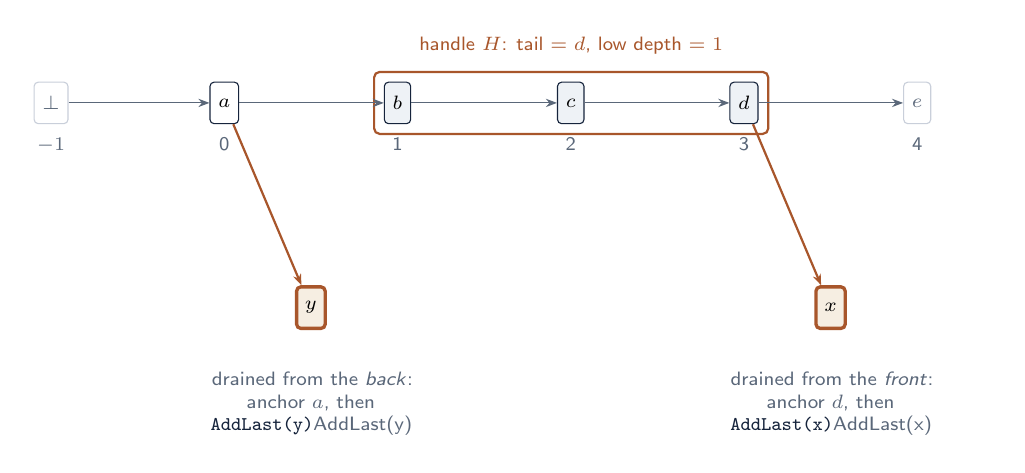
\begin{tikzpicture}[x=1mm,y=1mm]
  \node[d7ghost]    (bot) at (-55,0) {$\bot$};
  \node[d7node]     (a)   at (-33,0) {$a$};
  \node[d7leafnode] (b)   at (-11,0) {$b$};
  \node[d7leafnode] (c)   at ( 11,0) {$c$};
  \node[d7leafnode] (d)   at ( 33,0) {$d$};
  \node[d7ghost]    (e)   at ( 55,0) {$e$};
  \foreach \s/\t in {bot/a, a/b, b/c, c/d, d/e} \draw[d7edge] (\s) -- (\t);
  \foreach \n/\dd in {bot/{$-1$}, a/{0}, b/{1}, c/{2}, d/{3}, e/{4}}
    \node[d7label,below=1.5pt] at (\n.south) {\dd};
  \begin{scope}[on background layer]
    \node[draw=d7copper, thick, rounded corners=2pt, inner sep=3.5pt,
          fit=(b)(c)(d)] (win) {};
  \end{scope}
  \node[d7label,above=2.5pt,text=d7copper,align=center] at (win.north)
    {handle $H$: tail $=d$, low depth $=1$};
  \node[d7newnode] (y) at (-22,-26) {$y$};
  \node[d7newnode] (x) at ( 44,-26) {$x$};
  \draw[d7newedge] (a) -- (y);
  \draw[d7newedge] (d) -- (x);
  \node[d7label,anchor=north,text width=40mm,align=center] at (-22,-33)
    {drained from the \emph{back}:\\ anchor $a$, then \code{AddLast(y)}};
  \node[d7label,anchor=north,text width=40mm,align=center] at (44,-33)
    {drained from the \emph{front}:\\ anchor $d$, then \code{AddLast(x)}};
\end{tikzpicture}
\caption{The anchored-empty rule. The handle $H$ denotes $[b,c,d]$; node $e$ is
history below the window that $H$ cannot see. Emptying $H$ from either end
leaves the node immediately before the window as the anchor --- but that is $a$
in one case and $d$ in the other, so the two empty values append into different
branches. Both are empty, and neither can resurrect a discarded value.}
\label{fig:anchoredempty}
\end{figure}

\subsection{Which operations ask the arena}

The query discipline is stated exactly, because the difference between a
constant-time and a logarithmic operation here is precisely whether it needs an
ancestor.

\begin{d7tablethree}{0.34}{0.19}
\toprule
\thead{Operation} & \thead{Cost} & \thead{Shipped, Myers-backed} \\
\midrule
\code{AddLast} & $U$ & \bigoh{1} amortized \\
\code{Count}, \code{IsEmpty}, \code{Last} & \bigoh{1} & \bigoh{1} worst case \\
\code{RemoveFirst}, \code{RemoveLast}, \code{Drop}, \code{TryRemoveLast} & \bigoh{1} & \bigoh{1} worst case \\
\code{First}, indexer, \code{TryRemoveFirst} & $Q$ & \bigoh{\log M} worst case \\
\code{Take}, \code{Slice}, nontrivial \code{SplitAt} & $Q$ & \bigoh{\log M} worst case \\
enumerate $n$ visible values & $\Theta(n)$ & $\Theta(n)$ time, $\Theta(n)$ transient slots \\
\bottomrule
\end{d7tablethree}

\noindent
Two rows deserve comment. \code{Last} is free and \code{First} is not, which
looks like an asymmetry until one remembers what the handle stores: the tail is
a node, so its value is a direct read, while the front is an ancestor selected
jointly by the tail and the low depth. And \code{RemoveFirst} is free while
\code{TryRemoveFirst} is not, for the same reason --- the removal moves an
integer, but returning the removed value requires the query. Caching the front
would not fix this; it would only move the query into the next
\code{RemoveFirst}. Under a constant-query backend both become constant, which
is the whole argument for parameterizing the seam.

Boundary cases are specialized: \code{Take(Count)}, \code{Drop(0)}, a slice
whose result keeps the current tail, and a split at \code{Count} all return
without querying. The table gives the general case.

Enumeration walks parent links from the tail into a temporary array and yields
that array forwards, so it performs \emph{zero} ancestor queries at
$\Theta(n)$ time and $\Theta(n)$ transient slots. With a constant-query backend
one could instead run one query per output and keep \bigoh{1} iterator state.
Both are output-optimal in time; the transient-space difference is part of the
backend contract, and the shipped enumerator always buffers.

\section[The bilateral ancestral deque]{\code{BilateralAncestralDeque}}

\begin{specimen}[Specimen --- \code{BilateralAncestralDeque}]
\index{BilateralAncestralDeque@\texttt{BilateralAncestralDeque}}%
\spec{Purpose}{A fully persistent deque built from two oppositely oriented ancestry intervals, closed under reverse and arbitrary slicing.}
\spec{Core}{Two \term{segments} over one shared arena. A segment is (anchor, base, tail, count); the handle's value is the reversed left segment followed by the right one.}
\spec{Reverse}{\bigoh{1} --- the two segments change places. No flag, no rebuild.}
\spec{Ends}{Insertion at either end costs $U$. Both endpoint \emph{reads} are query-free.}
\spec{Removal}{\bigoh{1} on its own nonempty side; at most one query when it crosses the center.}
\spec{Index / slice}{At most one query to index; at most two to slice or split --- including when the range crosses the center.}
\spec{Limits}{No unrelated concatenation, no point replacement, no middle edit. Same retained-history model as the queue.}
\spec{Ports}{All nine.}
\end{specimen}

\noindent
The classical two-stack deque keeps a reversed front stack and a forward back
stack, and pays for the arrangement by occasionally transferring one stack into
the other. This structure keeps the arrangement and abolishes the transfer.

Each arm is an interval on some root-to-node path, exactly as in the queue, but
with two extra cached fields. Written $(\textsf{anchor}, \textsf{base},
\textsf{tail}, \textsf{count})$, the invariant is that the anchor is an ancestor
of the tail, that the count is the difference of their depths, and --- when the
arm is nonempty --- that the base is the anchor's child on that path, that is,
the first node strictly inside the interval. The handle's logical value is the
left arm read \emph{in reverse}, followed by the right arm read forwards.

Everything follows from that orientation. Adding at the front publishes a leaf
below the left tail; because the left arm is read in reverse, the newest node
reads first, which is precisely a prepend. Adding at the back publishes a leaf
below the right tail, which is an ordinary append. Removing from an arm's own
end moves its tail to its parent. Removing from the opposite side of an arm
advances its anchor to its cached base.

\subsection{Reverse is an exchange}

$\mathrm{reverse}(\mathrm{reverse}(L) \mathbin{+\!\!+} R) = \mathrm{reverse}(R)
\mathbin{+\!\!+} L$. The right-hand side is the representation of the handle
whose left arm is $R$ and whose right arm is $L$. So \code{Reverse} constructs a
new handle with the two segment records exchanged and the count unchanged: no
orientation flag to interpret at every subsequent call, no materialization, and
no lazy mirror to force. It is the cleanest reversal in the book, and it is
cheap for a structural reason rather than a bookkeeping one.

\subsection{Both ends, without asking}

The \textsf{base} field is redundant --- it is recoverable by a query --- and it
is the reason both endpoint reads are free. For the left arm the logical first
element is at the tail and the logical last is at the base; for the right arm
those roles are swapped. Whichever arm is empty, one of the four cached nodes
holds the answer, so \code{First} and \code{Last} are value reads.

That extends to indexing. Four positions are answered from cached endpoints with
no query at all: index $0$, the last index of the left arm, the first index of
the right arm, and the last index of the deque. Any other position costs exactly
one query --- into the left arm counting down from its tail, or into the right
arm counting up from its anchor.

It is worth putting this next to the queue, because the two structures made
opposite trades with the same budget. The queue does not cache its front, so
reading the front costs a query while advancing it is free. The deque caches its
bases, so reading either end is free while a removal that crosses the center ---
one that must retire an arm's base and cache the next one --- costs a query.
Neither is a mistake, and under an Alstrup--Holm backend the distinction
evaporates entirely; with the shipped arena it determines which of your
operations carry the logarithm.

\subsection{Slice closure, and the ceiling of two}

The central property is that the representation is \emph{closed} under
arbitrary contiguous slicing: a slice of a bilateral handle is another
bilateral handle, never a third fragment and never a rebuild. That is true
because a contiguous range intersects each arm in at most one contiguous piece.

The at-most-two-query ceiling follows from a case analysis that repays reading,
because the crossing case is the one that looks expensive and is not.

\begin{d7table}{0.30}
\toprule
\thead{The requested range} & \thead{What must move} \\
\midrule
Wholly inside one arm & Both endpoints of that arm's interval move; the other arm becomes empty. Two queries, fewer when a moved endpoint coincides with a cached one. \\
Crossing the center & The left intersection is a \emph{suffix} of the reversed left arm, so it keeps that arm's anchor and base and moves only its tail. The right intersection is a \emph{prefix} of the right arm, so it keeps that arm's anchor and base and moves only its tail. One query per arm. \\
Empty & No query. \\
\bottomrule
\end{d7table}

\noindent
So the expensive-looking case is the cheap one: crossing the center costs one
query in each arm precisely because each intersection inherits one of its
endpoints unchanged. \code{Take} and \code{Drop} are slices. \code{SplitAt} is
expressed as a \code{Take} plus a \code{Drop} and still makes at most two
queries in total, because the two results move complementary endpoints at the
same boundary. The focused test suites assert the exact maximum query count per
operation rather than a ceiling, which is how a claim like this stays true
through nine ports.

\begin{d7tablethree}{0.34}{0.24}
\toprule
\thead{Operation} & \thead{Cost} & \thead{Shipped, Myers-backed} \\
\midrule
\code{AddFirst}, \code{AddLast} & $U$ & \bigoh{1} amortized \\
\code{Count}, \code{First}, \code{Last}, \code{Reverse}, \code{Clear} & \bigoh{1} & \bigoh{1} worst case \\
\code{RemoveFirst}, \code{RemoveLast} & \bigoh{1}; at most one $Q$ across the center & \bigoh{1}; \bigoh{\log M} across the center \\
indexer & at most one $Q$ & \bigoh{\log M} worst case \\
\code{Take}, \code{Drop}, \code{Slice}, \code{SplitAt} & at most two $Q$ & \bigoh{\log M} worst case \\
\code{ToArray}, enumerate $n$ values & $\Theta(n)$, no queries & $\Theta(n)$ time, up to $\Theta(n)$ transient slots \\
\bottomrule
\end{d7tablethree}

\noindent
The deque handles empties differently from the queue, and the difference is
declared rather than incidental. An arm that empties while the other arm still
holds values collapses its anchor, base and tail onto one node and keeps it. But
a deque that empties completely --- and the value returned by \code{Clear} ---
resets both arms to the arena's bottom node, so the next insertion starts a
fresh branch at the root rather than continuing under an old anchor. Exact
anchor provenance is explicitly \emph{not} part of the deque's public value
semantics, where for the queue the anchoring rule is.

\section{What the family costs}

Both structures buy their bounds with the same three concessions, and the
proposals insist on them being visible.

\begin{caveatbox}[The logarithm is over the history, not the value]
Every \bigoh{\log M} in this chapter is logarithmic in $M$, the number of nodes
the arena has \emph{ever} published --- including nodes on branches no
application variable can still reach. It is not logarithmic in the length of the
handle you are holding. A thousand-element slice of a ten-million-append history
indexes at the cost of the history.
\end{caveatbox}

\begin{caveatbox}[Nothing is ever reclaimed, and one handle retains everything]
The arena keeps every node it has published, with its payload, until the arena
itself becomes unreachable. Dropping a prefix does not release nodes; releasing
a handle does not release nodes; garbage collection of a value must not be read
as reclamation of its history. And because every handle retains its arena, one
surviving handle retains the entire history --- which is normal for an
arena-backed persistent structure and unacceptable for an unbounded service.
Reclamation would require tracing from live handles, explicit epochs, or an
ancestor index that tolerates deletion. None of the three is here.
\end{caveatbox}

The third concession is the algebra. Neither structure concatenates unrelated
histories, replaces a point, or edits the middle, and neither is confluently
persistent: two versions that branched apart cannot be merged. Equality is a
further casualty --- two handles can enumerate identical values from different
tails, different anchors, or different arenas, so reference identity is neither
content equality nor a provenance test, and no constant-time sequence equality
or canonical empty is promised.

The concessions are the mechanism, not an accident of implementation. It is
exactly because there is no concatenation and no point update that a value can
be two boundaries on somebody else's path, and exactly because a value is two
boundaries that indexing and slicing reduce to one ancestor query apiece. When
the missing operations are needed, the library says so plainly and points at the
general structures: \code{FingerTreeDeque} (Chapter~\ref{ch:fingertree}) for a
persistent sequence with concatenation and arbitrary edits, and
\code{ReversibleDeque} (Chapter~\ref{ch:revdeque}) when reversal is the primary
operation over a full sequence algebra. These two are justified only
when branching append histories with subrange and indexed access dominate, and
when the operations they do not have are genuinely unnecessary.


\chapter{Lifting a Machine into a Measure}
\label{ch:contextual}

\motto{When a summary cannot know what came before it, make it answer for every
possible before.}

\begin{specimen}[Specimen --- \code{ContextualRankSequence}]
\index{ContextualRankSequence@\texttt{ContextualRankSequence}}%
\spec{Purpose}{A persistent sequence that ranks and selects \emph{events} whose occurrence depends not on an element alone but on the finite context preceding it --- the comma that separates fields here and is quoted data there.}
\spec{Core}{The measured finger tree under a lifted measure: for every subtree \emph{and every one of the machine's states}, the outgoing state and the number of events emitted.}
\spec{Algebra}{A finite deterministic machine over $s$ states emitting nonnegative event counts. The lifted summary is an ordered monoid --- associative, and emphatically not commutative.}
\spec{Operations}{\code{Evaluate}, \code{EvaluatePrefix}, \code{EventRank}, \code{TrySelectEvent}, over the ordinary positional surface: index, insert, replace, remove, split, slice, concatenate.}
\spec{Complexity}{\bigoh{1} whole-sequence evaluation; \bigoh{s \log n} amortized for prefix evaluation, rank, select, and every edit; \bigoh{s} amortized endpoint updates; \bigoh{s \log \min(n,m)} amortized concatenation; \bigoh{s n} to build and to store.}
\spec{Policies}{The machine is compile-time in C\#, C\texttt{++}, and Rust; a retained runtime object in Kotlin, TypeScript, and Python; a record of functions in Haskell; an identified callback struct in C and OCaml.}
\spec{Ports}{All nine.}
\end{specimen}

\noindent
Every measure in Chapter~\ref{ch:measures} shares an assumption so quiet that it
is easy to miss: an element's contribution to the summary is a property of the
element. A character contributes one to a length; a key contributes itself to a
maximum; a newline contributes one to a line count. Nothing about the neighbors
enters into it, which is exactly why the contributions can be combined in any
grouping and cached on every subtree.

Now take a rule that breaks the assumption. In a CSV line, a comma is a field
separator --- unless it falls inside a quoted field, in which case it is data. The
element is identical in both cases. What differs is everything that came before
it. No fixed weight is correct for a comma, so no ordinary measure can rank
commas, and the whole apparatus of measure-guided descent is unavailable for a
question that is otherwise a textbook rank-and-select.

This chapter is about the way out, and it is the most elegant construction in the
repository.

\section{Why the obvious repairs are linear}

Keep the characters in any persistent sequence and run a two-state scanner over
them. That works, and it is what almost everyone does. Its cost is structural:
to know whether the comma at position $i$ is a separator you must know the
scanner's state entering position $i$, and that state is a function of all $i$
preceding characters. Asking for the event rank at a boundary $p$ costs
$\Theta(p)$; asking which element emitted the $k$-th event costs $\Theta(n)$ in
the worst case; and a single insertion at the front invalidates the entering
state of everything after it.\index{contextual rank}

The tempting fix --- cache the entering state on each node --- fails for the same
reason, and it fails completely rather than partially. A cached entering state is
valid for exactly one prefix. Prepend one quotation mark and every cached entry
in the tree is wrong. What is expensive here is not the scan; it is the
\emph{dependence of the cache on the prefix}. Any repair that leaves that
dependence in place will be linear in disguise.

Binary search does not rescue it either. One could search for the boundary at
which the running event count first exceeds $k$, but evaluating the predicate at
a candidate boundary is itself a prefix replay, so the first probe alone costs
$\Theta(n)$.

\section{The lift}

\code{ContextualRankSequence<TElement, TMachine>} removes the dependence instead
of trying to maintain it. Its measure caches not the answer, but the answer
\emph{as a function of the entering state}.\index{effect table}

The policy supplies a finite deterministic machine: a state count $s$, and a
transition that consumes one element from one state and reports the outgoing
state together with a nonnegative count of emitted events. A subtree's summary
--- its \term{effect table} --- is then two arrays of length $s$ plus the ordinary
element count:

\begin{center}
\fbox{\parbox{0.86\linewidth}{\centering\vspace{2pt}
$A.\mathrm{next}(q)$ --- the state after consuming $A$ from $q$\\
$A.\mathrm{events}(q)$ --- the events emitted while consuming $A$ from $q$
\vspace{2pt}}}
\end{center}

\noindent
tabulated for every $q$ in $0 \ldots s-1$. Ordered composition feeds the left
table's outgoing state into the right table:

\begin{align*}
(A \otimes B).\mathrm{next}(q)   &= B.\mathrm{next}(A.\mathrm{next}(q)) \\
(A \otimes B).\mathrm{events}(q) &= A.\mathrm{events}(q) + B.\mathrm{events}(A.\mathrm{next}(q)) \\
(A \otimes B).\mathrm{count}     &= A.\mathrm{count} + B.\mathrm{count}
\end{align*}

The identity maps every state to itself, emits nothing, and holds no elements.
That is a monoid, and a monoid is precisely what the measured finger tree wants.
Associativity is not a coincidence and needs no clever argument: the state
component is function composition, which is associative, and the event component
is a sum of terms each indexed by the state its subtree is entered in, so both
parenthesizations end at
$C.\mathrm{next}(B.\mathrm{next}(A.\mathrm{next}(q)))$ with the identical three
event terms. The algebraic shape is the machine's transition monoid decorated
with additive output --- the same object one composes when composing
deterministic weighted transducers, in Mohri's sense.\index{transition monoid}

\begin{figure}[htbp]
\centering
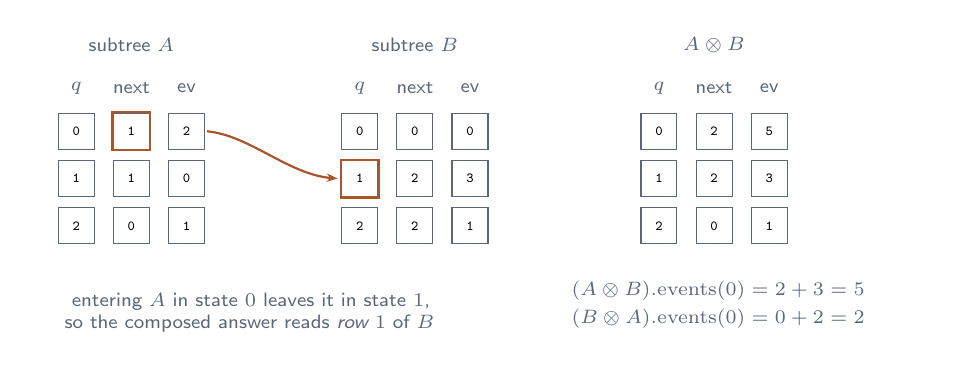
\begin{tikzpicture}[x=1mm,y=1mm]
  \node[d7label] at (-31,9) {subtree $A$};
  \node[d7label] at (5,9) {subtree $B$};
  \node[d7label] at (43,9) {$A \otimes B$};
  \foreach \x in {-38,-2,36} \node[d7label] at (\x,3.5) {$q$};
  \foreach \x in {-31,5,43}  \node[d7label] at (\x,3.5) {next};
  \foreach \x in {-24,12,50} \node[d7label] at (\x,3.5) {ev};

  \foreach \yy/\qq/\nn/\ee in {-2/0/1/2, -8/1/1/0, -14/2/0/1} {
    \node[d7cell] at (-38,\yy) {\qq};
    \node[d7cell] at (-31,\yy) {\nn};
    \node[d7cell] at (-24,\yy) {\ee};
  }
  \foreach \yy/\qq/\nn/\ee in {-2/0/0/0, -8/1/2/3, -14/2/2/1} {
    \node[d7cell] at (-2,\yy) {\qq};
    \node[d7cell] at (5,\yy)  {\nn};
    \node[d7cell] at (12,\yy) {\ee};
  }
  \foreach \yy/\qq/\nn/\ee in {-2/0/2/5, -8/1/2/3, -14/2/0/1} {
    \node[d7cell] at (36,\yy) {\qq};
    \node[d7cell] at (43,\yy) {\nn};
    \node[d7cell] at (50,\yy) {\ee};
  }

  \draw[d7copper,thick] (-33.4,-4.4) rectangle (-28.6,0.4);
  \draw[d7copper,thick] (-4.4,-10.4) rectangle (0.4,-5.6);
  \draw[d7newedge] (-21.4,-2) .. controls (-16,-2.5) and (-11,-7.5) .. (-4.8,-8);
  \node[d7label,align=center,text width=54mm] at (-16,-25)
    {entering $A$ in state $0$ leaves it in state $1$, so the composed
     answer reads \emph{row $1$} of $B$};
  \node[d7label,anchor=west,align=left,text width=44mm] at (24,-24)
    {$(A \otimes B).\mathrm{events}(0) = 2 + 3 = 5$\\[2pt]
     $(B \otimes A).\mathrm{events}(0) = 0 + 2 = 2$};
\end{tikzpicture}
\caption{An effect table is a subtree's entire behavior, tabulated for every
state it might be entered in. Composition uses the left table's outgoing state as
a row index into the right table --- which is why the order of the operands
matters, and why no part of the construction ever needs to know the real entering
state in advance.}
\label{fig:effecttable}
\end{figure}

The $s$ columns are the price of not knowing the prefix, and it is worth naming
the trade plainly: a factor of $s$ in storage and in every composition buys the
disappearance of the prefix dependence. Nothing else changes. The tree is the
same measured finger tree that carries a size or a maximum; only the monoid is
new.

\subsection{Not commutative, and it matters}

Effect-table composition is associative but decidedly not
commutative.\index{monoid!associativity} $A \otimes B$ and $B \otimes A$
generally disagree in \emph{both} components --- in Figure~\ref{fig:effecttable}
they report event counts of five and two from the same starting state. The left
operand chooses which row of the right operand's table is read, and swapping the
operands changes the choice.

This is not a footnote. A measured tree that combines summaries in any order
other than sequence order, or that reuses a cached summary for a subtree it has
mirrored, silently produces a wrong answer here, and the answer is wrong in a way
no type checker sees. The library is scrupulous about ordered combination for
exactly this class of measure, and the discipline has been tested by events: when
the complexity-parity campaign gave the deques an \bigoh{1} lazy reversal,
Python's first implementation reused each mirrored node's cached summary ---
correct only when \code{Combine} is commutative --- and was rewritten to match
TypeScript's, which recombines the mirrored parts in mirrored order and is
correct under every monoid, verified by a probe whose measure is a string and
whose combine is concatenation. The contextual sequence is the kind of measure
that makes that difference matter.

\section{Rank and select in one descent}

Because event counts are nonnegative, the running event total is monotone along
the sequence, and so the predicate
\[
  P.\mathrm{events}(q_0) > r
\]
is false and then true as prefixes grow --- a lawful split predicate in the sense
of Chapter~\ref{ch:measures}. Selecting the element that emitted event $r$ is
therefore one measure-guided descent, with no binary search over boundaries and
no prefix replay anywhere.\index{measure!guided descent}

What comes back is not merely an index. The summary immediately before the
located element already contains everything the caller needs, so
\code{TrySelectEvent} reports five things at once: the index of the emitting
element, the event's ordinal within that element's transition (a single
transition may emit several events), the machine state before the element, the
state after it, and the transition's total event count. Rank is the same descent
stopped at a boundary: \code{EventRank} is \code{EvaluatePrefix}'s event
component, and the two are exact inverses --- adding the ordinal within the
transition to the preceding prefix's count reconstructs $r$.

Notice which argument the initial state is. It is a parameter of the
\emph{query}, not of the structure. Because every subtree is tabulated for every
state, the same stored sequence answers ``what if the scanner arrives here
already inside a quoted field?'' at no extra cost and with no rebuild.

\subsection{A scanner, and its answers}

The machine that motivates the structure is two states wide.

\begin{lstlisting}[language={[Sharp]C}]
readonly struct QuotedComma : IContextualEventMachine<char>
{
    public static int StateCount => 2;   // 0 = outside quotes, 1 = inside

    public static ContextualEventTransition Transition(int state, char value) =>
        value switch
        {
            '"' => new(1 - state, 0),             // toggle, emit nothing
            ',' when state == 0 => new(state, 1), // a real separator
            _ => new(state, 0)
        };
}

var text = ContextualRankSequence<char, QuotedComma>.Create("\"a,b\",c,d".AsSpan());
\end{lstlisting}

\noindent
Index those nine characters from zero: the quotation marks are at positions~0
and~4, and the commas at 2, 5, and~7. One of the three commas is data and two are
separators, and the structure knows which is which from either starting context:

\begin{lstlisting}[language={[Sharp]C}]
text.Evaluate(0);      // (FinalState 0, EventCount 2)
text.Evaluate(1);      // (FinalState 1, EventCount 1)
text.EventRank(5, 0);  // 0 -- no separator among the first five characters
text.EventRank(6, 0);  // 1

text.TrySelectEvent(0, 0, out var first);
// (ElementIndex 5, EventIndexInElement 0, StateBefore 0, StateAfter 0,
//  ElementEventCount 1)

text.TrySelectEvent(0, 1, out var other);
// other.ElementIndex == 2 -- entering mid-quote, the inner comma is the separator

var edited = text.Insert(0, '"');
// text is unchanged; edited ranks every later comma differently
\end{lstlisting}

Read the last two calls together. From the outside, the first separator is the
comma at index~5 and the comma at index~2 is data. Entering already inside a
quoted region, the first separator \emph{is} the comma at index~2 --- and the
answer comes from the same cached tables that produced the first one, in one
descent, with the machine consulted at most once. Prepending a quotation mark
produces a new version with different ranks throughout while leaving the original
version and its cached answers exactly as they were.

\subsection{Writing your own machine}

The recipe generalizes to anything expressible as a finite deterministic
transducer with nonnegative output counts, and the proposal lists the family the
design was drawn from: token or record boundaries in a finite-state lexer, frame
boundaries in an escaped byte stream, delimiters outside quoted or commented
regions, transitions into a selected protocol or workflow state, and Unicode text
boundary policies once compiled to a finite-state machine --- Annex~\#29 calls out
the random-access difficulty explicitly, and this is one answer to it.

Four obligations make a machine lawful. Bound the context, so that a state count
exists at all. Make the transition total and deterministic on every state, not
merely on the states you expect to reach. Emit nonnegative counts, or select
stops being monotone and the descent stops being meaningful. And if the rule
needs \emph{right} context, compile it into a streaming machine or pair it with a
reverse machine yourself --- the structure does not hide that transformation, and
says so.

\begin{asidebox}[Every state, not just the reachable ones]
Because a leaf's table is filled for all $s$ states when the element is stored,
the transition is validated for all $s$ states too. A machine that returns an
out-of-range state or a negative count only from state~3 is rejected the moment
an element is inserted, even if no version of the sequence ever enters state~3.
The failure surfaces where the bug is, not months later in a query.
\end{asidebox}

\section{What it costs}

Let $n$ be the element count and $s$ the machine's state count.

\begin{d7tablethree}{0.30}{0.27}
\toprule
\thead{Operation} & \thead{Bound} & \thead{Why} \\
\midrule
\code{Evaluate} & \bigoh{1} & one read of the cached root table \\
\code{EvaluatePrefix}, \code{EventRank} & \bigoh{s \log n} amortized &
\bigoh{\log n} levels, one \bigoh{s} composition each; \bigoh{1} at either
endpoint \\
\code{TrySelectEvent} & \bigoh{s \log n} amortized & one monotone descent \\
Indexing, \code{SetItem}, \code{Insert}, \code{RemoveAt}, \code{SplitAt},
\code{GetRange} & \bigoh{s \log n} amortized & measured locate or split, then a
path copy \\
\code{Prepend}, \code{Append} & \bigoh{s} amortized, \bigoh{s \log n} worst case
per call & digits absorb the work; see below \\
\code{Concat} & \bigoh{s \log \min(n,m)} amortized & the suspended middle
recursion stops at the shallower operand \\
\code{Create}, \code{CreateRange} & \bigoh{s n} & one table per element \\
Enumeration & \bigoh{n} & a traversal stack, composing nothing \\
Storage & \bigoh{s n} & every node and every element caches an $s$-wide table; a
changed spine adds \bigoh{s \log n} \\
\bottomrule
\end{d7tablethree}

\noindent
Two of those rows deserve their fine print. The whole-sequence \code{Evaluate} is
\bigoh{1} in the reference because the wrapper forces the root summary before
publishing a version --- the same forcing that makes a faulty machine fail before
any successor becomes visible. The TypeScript port states the same operation as
\bigoh{1} amortized on the ground that the first read of a freshly built spine
may force its suspended middles once. The two ports are charging the same
one-time work at different moments; the second wording is the more careful one.

And the \bigoh{s n} storage should be read with its quantifier in place. For a
fixed machine, $s$ is a constant: the contextual queries are \bigoh{\log n} and
the storage is \bigoh{n}, which is why the structure is worth having at all. If
instead $s$ is treated as an input, the library is explicit that this structure
does \emph{not} dominate a plain persistent sequence --- its edits and its storage
carry the $s$ factor openly, and a machine with a thousand states will feel like
one.

\section{Why this chapter is the parity campaign's best exhibit}

Look again at the two rows that make this structure attractive rather than merely
correct: \bigoh{s} amortized endpoint updates and \bigoh{s \log \min(n,m)}
concatenation. Neither is a property of the effect-table monoid. Both are
properties of the substrate underneath it, and they hold only on a genuine lazy
Hinze--Paterson finger tree --- digits at both ends to absorb an endpoint push in
constant node work, and a memoized suspension in every deep node's middle so that
the amortization survives \emph{persistent branching} rather than merely
ephemeral linear use (Chapter~\ref{ch:laziness}).\index{laziness}\index{amortization!under persistence}

For a period, four of the nine ports could not state them. Rust, Kotlin, OCaml,
and Python shipped this collection over height-balanced join trees --- one element
per node, cached measures, no digits and no suspensions --- and each documented
$\Theta(s \log n)$ endpoints and a concatenation bound keyed to how the two
operands' shapes compared rather than to the smaller of them --- a height
difference in three of the ports, a weight ratio in weight-balanced
OCaml. Those were honest notes, not bugs, and they were
measured rather than assumed: instrumenting Python's summary combiner showed a
16{,}384-element sequence concatenated with a small one costing 28 compositions
whether the small operand held 1 element or 1{,}024, which is the signature of a
height-difference bound rather than a $\log \min$ one. All four carried
substrate-divergence notes until their cores were rebuilt.\index{complexity parity}

Wave~1 of the complexity-parity campaign replaced all of those cores in place,
and every one of the four now states the reference's bounds with a probe behind
them; the campaign's core measurements show concatenation of a 4{,}096-element
tree costing zero immediate combines against a one-element operand and four
against a 1{,}024-element one --- cost tracking the smaller operand, not the
height difference. TypeScript, ported last, is the only port that never had to
weaken the claim in the first place.

The lesson generalizes past this one collection. A structure inherits its
guarantees from whatever it is built on, and a collection can be entirely correct
--- passing every behavioral test, in every language --- while quietly failing the
bound that was the reason to choose it. That is the argument for the campaign in a
single example.

\begin{caveatbox}[Where the ports still differ]
Three differences survive, all documented at their own function. Haskell's
enumeration is $\Theta(s \cdot n)$ rather than \bigoh{n}, because its measured
core's left-view fold rebuilds a spine node per step and each rebuild forces a
fresh \bigoh{s} composition, where the reference's enumerator walks a traversal
stack and combines nothing. Ports whose measured core carries an explicit element
count alongside the measure --- Rust, Kotlin, OCaml, Python, TypeScript --- answer
a positional index in \bigoh{\log n} composing no table at all, which is better
than the reference's measure-directed \bigoh{s \log n}. And the ports that store
each element's effect row beside the element (Kotlin, Python, TypeScript) invoke
the machine \emph{zero} times on a successful select, where C\# and Rust invoke it
exactly once to report the located transition.
\end{caveatbox}

\section{Where the guarantees stop}

\begin{caveatbox}[Deliberate limits]
\textbf{Context must be finite.} Parenthesis depth, indentation stacks, and
general parsers do not fit unless their state is explicitly bounded. The state
count is validated once and then fixed for the lifetime of the sequence.

\textbf{Context flows left to right.} A right-context rule must be compiled into a
streaming machine, delayed, or paired with a reverse machine by the caller.

\textbf{Event weights must be nonnegative}, or the select predicate stops being
monotone and measure-guided descent stops being sound.

\textbf{Totals are checked.} Event counts accumulate in a checked 64-bit
integer and element counts in a 32-bit one; a version whose composed total would
overflow is rejected rather than wrapped. Haskell, whose counts are unbounded
integers, keeps the negative-count rejection and drops the vacuous overflow
contract.

\textbf{One element per measured leaf.} This is not a chunked text rope and makes
no cache-density claim.

\textbf{The machine cannot be changed.} Concatenation requires identical machine
semantics, enforced by the type system where a type system can carry the policy
and by retained-policy or identifier equality where it cannot. Rebuilding an
existing sequence under a different machine costs \bigoh{s n}.
\end{caveatbox}

\begin{contractbox}[Failure atomicity]
Every operation builds its complete successor before returning it. A throwing
transition, an out-of-range next state, a negative event count, or an overflowing
total publishes no successor, and every retained version remains exactly as it
was. In C\# one wrinkle is worth knowing in advance: because the machine's state
count is validated in the closed generic type's static initializer, a nonpositive
state count reaches the caller as a \code{TypeInitializationException} whose inner
exception carries the real diagnostic, and every later use of that same
constructed type reports the same wrapped failure. That is how the runtime
reports faulted static initialization; the type is documented to be read through
its inner exception.
\end{contractbox}

\section{On novelty, stated narrowly}

The repository is careful about what it claims here, and the care is worth
reproducing. Every ingredient is established: Driscoll, Sarnak, Sleator, and
Tarjan formalized persistence; Hinze and Paterson supplied the measured sequence
and the monotone measure-guided split; Frandsen, Miltersen, and Skyum studied
updates and prefix products in a fixed finite monoid under the name of dynamic
word problems; Mohri's survey covers weighted transducer composition. The lift is
mathematically natural the moment weighted deterministic transitions and measured
trees are set side by side, and a tree that already stored exactly these arrays
with exactly this predicate would be this construction under another name.

What the proposal records is therefore a deliberately small claim: a reproducible
negative search result --- that the searched primary sources did not expose this
particular public synthesis of a fully persistent, insert-and-concatenate-capable
sequence with all-start-state additive summaries and one-descent contextual
rank and select that reports the emitting input position. Not a priority claim,
not a patentability claim. An earlier or differently named instance may exist. It
is a good habit, and this is the collection that most tempts one to break it.


\chapter{Checkpoints and Deltas}
\label{ch:checkpoint}

\motto{Two roots prove that a version changed. Neither says where.}

\noindent
Persistence makes versions cheap. Keep the old root, edit the new one, and both
remain readable forever at the cost of a path copy. What persistence does not do
by itself is answer the question a caller asks immediately afterwards:
\emph{which} keys --- or which positions --- differ from the version I nominated
as my baseline, and what did they hold before?\index{checkpoint}

There are two obvious ways to answer it, and both are unsatisfying for the same
reason. The first is to compare the two roots. That is correct, and a
sharing-aware comparison can be very fast when the two versions share most of
their structure, but its cost is set by the \emph{representation} rather than by
the size of the answer: a single edit path-copies its whole spine, so even one
change leaves a logarithmic frontier of unshared nodes for a differ to walk. The
second is to keep a write log. A log is cheap to append and names every
operation, but it names operations rather than net effect --- repeated writes to
one key, a value that travels away and comes back, and the order a consumer
should read the result in are all left to be resolved later, at a cost
proportional to the log rather than to the difference.

The two structures in this chapter take a third route. They maintain the exact
net answer \emph{online}, while the edits are happening, so that asking the
question later is a read rather than a computation. They differ in what they
index: one records a change per changed key, the other records a change per
contiguous \emph{run} of changed positions, which is the right granularity when
the state is a slab rather than a sparse keyspace.\index{delta}

Both began as research prototypes with normative design proposals of their own,
were promoted out of the library's experimental namespaces once those proposals
had been reviewed, and now ship in all nine languages.

\section{The checkpoint-differential map}

\begin{specimen}[Specimen --- \code{PersistentDeltaMap}]
\index{PersistentDeltaMap@\texttt{PersistentDeltaMap}}%
\spec{Purpose}{A fully persistent ordered map that also knows, at every moment, exactly which key classes differ from its own checkpoint and what their checkpoint and current values are.}
\spec{Core}{Three immutable roots --- checkpoint state $B$, current state $S$, and an ordered change index $D$ carrying one presence-safe \code{(before, after)} record per key class on which $B$ and $S$ differ. All three are persistent sorted maps under the same key comparer.}
\spec{Operations}{\bigoh{\log N} lookup, point update, removal, rank, and neighbor queries, where $N$ counts the key classes in $\mathrm{dom}(B) \cup \mathrm{dom}(S)$ --- the same bounds as the ordinary ordered map underneath.}
\spec{Epoch control}{\code{Checkpoint} and \code{Rollback} are \bigoh{1}. They exchange roots; they do not scan.}
\spec{Enumeration}{$\Theta(k + 1)$ to fully consume all $k$ changes in ascending key order. The range-restricted overload seeks in \bigoh{\log(k+1)} and then costs $\Theta(1)$ per change yielded.}
\spec{Policies}{A key comparer defining order \emph{and} identity, and a value equality relation defining semantic no-ops and cancellation.}
\spec{Limits}{Point mutation only. No \code{Clear}, no bulk or range update, no diff between two arbitrary retained versions, no confluent merge.}
\spec{Ports}{All nine.}
\end{specimen}

\noindent
The shape of the design is visible in the field list: a version is a wrapper
around three roots and a policy. $S$ answers every ordinary map question and
delegates to the underlying sorted dictionary without ceremony. $B$ is shared,
not copied --- it is simply the state root some ancestor version published as
its baseline. $D$ is where the work lives.\index{change index}

What makes $D$ worth maintaining is that it holds the \emph{net} answer, not a
history. Four rules produce that, and each one is a specific decision that could
plausibly have gone the other way.

\begin{contractbox}[The four rules that make ``net'' exact]
\textbf{A relation-equal write is a semantic no-op.} Writing a value that the
retained value relation calls equal to the value already stored returns the
receiver unchanged --- the same object, not an equal one. No record is created,
none is disturbed, and no successor is allocated. Removing an absent key behaves
the same way.

\textbf{The first effective write captures \code{before}.} When a key class
enters $D$, the endpoint it records as \code{before} is the checkpoint-relative
state it is about to displace: \code{Present(v)} if the class was in the
checkpoint, \code{Absent} if it was not. Presence is carried separately from the
value, so \code{Present(null)} and \code{Absent} are distinguishable --- a
distinction the ports without a null-inhabited type spell as \code{Option} or
\code{Maybe}.

\textbf{Repeated writes coalesce.} Every later effective write to that class
replaces only \code{after}; the captured \code{before} is never rewritten. A
class written a thousand times still occupies one record, holding the first
checkpoint-relative endpoint and the final current one.

\textbf{Returning a key to its checkpoint state deletes its record.} After each
effective write the two endpoints are compared --- presence first, then the
value relation when both are present --- and if they agree the record is
\emph{removed} rather than stored as a zero. A complete
$v_0 \to v_1 \to v_0$ round trip therefore leaves no trace, and $D$ never
contains a record that is not a real difference.
\end{contractbox}

The fourth rule has a consequence worth spelling out, because it is the one that
makes the structure feel different in use: the change set can shrink. An epoch
that touches five hundred keys and then puts four hundred and ninety of them
back holds ten records, and \code{ChangeCount} reads that ten as an amortized
\bigoh{1} field rather than recounting anything.

\subsection{Canonicalization: a cancelled epoch is storage-clean}

If the last surviving record is removed --- if the whole epoch cancels --- the
successor does not merely hold a current root that is extensionally equal to the
checkpoint. It holds the checkpoint root \emph{itself}. The state root snaps
back, and both logical views name one object again.\index{canonicalization}

This is not needed for the \bigoh{1} bound on \code{Checkpoint} and
\code{Rollback}; those allocate a constant-size wrapper in any case. What the
snap buys is that a wholly cancelled epoch is storage-clean as well as
extensionally clean. The identity test at the head of \code{Checkpoint} and
\code{Rollback} then recognizes the version as already clean and returns the
receiver rather than a fresh wrapper, and a later root-identity equality test
against the baseline settles in constant time instead of walking an unshared
path that a state-only path-copied map would have left behind.

The snap is also the place where the representative rule earns its keep, and it
is subtler than it looks. Because the key comparer defines identity, several
distinct key objects can name one class, and the map must decide which
representative it stores. A changed class that existed in the checkpoint retains
the checkpoint's representative through updates and through delete/re-add round
trips; a class absent from the checkpoint retains the first insertion's
representative for as long as its net-added record survives, and a later
insertion after complete cancellation begins a fresh episode. That rule is what
makes the snap sound: when $D$ empties, current and checkpoint agree not only
extensionally but representative-wise, so substituting one root for the other
changes nothing a caller can observe.

\begin{lstlisting}[language={[Sharp]C}]
var map = PersistentDeltaMap<string, int>.CreateRange(
    [new("a", 1), new("b", 2), new("c", 3)]);

var edited = map.SetItem("b", 20)   // Updated: Present(2) -> Present(20)
                .SetItem("b", 21)   // coalesces; before is still Present(2)
                .Remove("c")        // Removed: Present(3) -> Absent
                .SetItem("d", 4);   // Added:   Absent     -> Present(4)

var count = edited.ChangeCount;     // 3, not 4: the two writes to "b" coalesced
foreach (var change in edited.GetChanges())
{
    // ("b", Present(2), Present(21))
    // ("c", Present(3), Absent)
    // ("d", Absent,     Present(4))   -- ascending key order, once each
}

var restored = edited.SetItem("b", 2);   // b's record is deleted: 2 changes
var clean    = edited.Rollback();        // O(1); map, edited, restored survive
\end{lstlisting}

\subsection{Why the enumeration is the point}

The change index holds exactly $k$ records, so any operation that visits all of
them has an information-theoretic $\Omega(k)$ output cost. An in-order walk of
$D$ costs $\Theta(k + 1)$ --- the $+1$ is enumerator setup --- and is therefore
output-optimal.\index{output-optimal} It invokes no key or value policy callback
at all: the ordering work was done when the records were inserted.

The comparison worth making is against the alternative the structure exists to
replace: reconstructing the same change set from two state-only path-copied
trees by pruning at reference-equal subtrees. That technique is genuinely good
and is what a library like Rust's \code{im} offers, but its cost is the number
of nodes the two operands do \emph{not} share, and a point edit necessarily
copies its own search spine. Take a complete fixed-fanout tree with $N$ leaf key
classes and change $k$ leaves spaced evenly through key order. The union of the
copied root-to-leaf paths contains $\Theta(k)$ nodes above the point where the
paths separate plus $\Theta(k \log(N/k + 1))$ nodes in the $k$ disjoint lower
spines, so a differ whose only certificate of ``unchanged'' is node identity
must inspect a $\Theta(k \log(N/k + 1))$ frontier. At $k = 1$ that is
$\Theta(\log N)$ nodes walked to report one change; the delta map reports it in
$\Theta(1)$.\index{adversary argument}

The library is careful about what this does and does not claim. It is not a
universal lower bound on change discovery. Canonical hashing, hash-consing,
per-version logs, or any other maintained metadata changes the problem --- and
the delta map is itself exactly such an auxiliary index. What it claims is the
trade: the reconstruction work is moved forward into \code{SetItem} and
\code{Remove}, where it costs one extra ordered-map edit --- and since $k \leq N$
that edit's \bigoh{\log(k + 1)} is inside the state edit's \bigoh{\log N},
changing the constants of a point update but not its asymptotic, and buying an
output-optimal query in exchange. Liljenzin's confluent persistent maps, and the
Blelloch--Reid-Miller and ``Just Join'' set-operation results, solve a strictly
broader problem --- arbitrary operands, confluent combination --- and their
$\Theta(m \log(n/m + 1))$ bound is in the smaller \emph{input} size, not in this
structure's output size $k$. They do not contradict the $\Theta(k + 1)$ here,
because the delta map is allowed to remember things while the edits happen.

\subsection{The range-restricted overload is a seek, not a filter}

\code{GetChanges(low, high)} yields the changes whose keys fall in an inclusive
range, in the same ascending order. The important property is that it is a
genuine boundary seek: the change index is itself an ordered map under the
collection's key comparer, so restricting it is two boundary descents plus a
bounded walk of the in-range sub-map. The bound is \bigoh{\log(k + 1)} for the
seek --- performed on first enumeration, and invoking only key-order comparisons
--- plus $\Theta(1)$ per change actually yielded. A window of four changes in an
index of two thousand costs what four changes cost, not what two thousand cost.

That distinction is not academic, and the library has the scar tissue to prove
it. The C port's header promised the boundary-only comparison bound while its
walk compared at every visited node --- $\Theta(\text{output} + \log k)$
comparator invocations, observable through a counting comparer --- and the
cross-language parity audit caught it. The walk was rewritten to propagate
established bounds, so comparisons now occur only along the two boundary paths
and the in-range interior is traversed comparison-free; the comparison-count
test that guards it was tightened from 512 to 96. Haskell shipped a differently
flawed version of the same idea: a real seek, but with a logarithmic per-element
term rather than a constant one, because its shared sorted map exposed no
key-range restriction at all. Adding one gave the delta map the baseline's shape
and dropped a measured four-element window over a 2{,}048-record change index
from 61 key comparisons to 22. Every port written afterwards states explicitly
that its range enumeration is a seek through the substrate's own range
restriction, and pins the claim with a mutation that reintroduces the filter and
must fail.

\begin{caveatbox}[There is no \code{Clear}, and that is deliberate]
Clearing a checkpoint of $N$ keys creates $N$ net removal records. Maintaining
$D$ eagerly through that costs $\Theta(N)$ time and space, and no lazy
representation can both keep the explicit-record invariant and match an ordinary
immutable map's root-dropping \bigoh{1} clear. Rather than ship a method whose
cost violates the structure's own no-regression premise, the API omits it: start
a fresh epoch from \code{Create} when no old-to-new patch is wanted, or remove
entries explicitly when one is. Bulk set, union, merge, range mutation, and
\code{Diff(otherVersion)} are absent for related reasons. \code{SetItems} exists,
but it is documented as exactly the left fold of \code{SetItem} --- an allocation
saving, not a different algorithm --- so every coalescing, cancellation, and
representative rule holds verbatim through it.
\end{caveatbox}

A live version retains \bigoh{N + k} nodes: two state snapshots and a $k$-entry
index, usually far less physically because of sharing. Retaining every successor
adds \bigoh{\log N} nodes per changed point update --- the same asymptotic
version-retention cost as an ordinary path-copied ordered map, with a roughly
doubled constant for the second tree.

\section{The run-delta vector}

\begin{specimen}[Specimen --- \code{PersistentRunDeltaVector}]
\index{PersistentRunDeltaVector@\texttt{PersistentRunDeltaVector}}%
\spec{Purpose}{A fixed-length persistent vector with a checkpoint, indexing the exact \emph{maximal contiguous runs} of positions whose current values differ from that checkpoint --- and able to accept or revert one whole run.}
\spec{Core}{Two equal-length immutable RRB vectors, current and checkpoint, plus a persistent ordered map holding one \code{start} $\to$ \code{endExclusive} record per maximal dirty run, plus a cached dirty-position count.}
\spec{Operations}{\bigoh{\log n} indexed read of either view; \bigoh{\log n} point edit; \bigoh{\log(r+2)} dirty membership and run-by-rank selection over $r$ runs; \bigoh{1} fork, checkpoint, and rollback.}
\spec{Enumeration}{$\Theta(r)$ run descriptors --- output-optimal --- against worst-case $\Theta(n)$ discovery from unindexed roots. Complete value enumeration is still \bigoh{n}.}
\spec{Hunks}{Accepting or reverting one indexed run is \bigoh{\log n} through structural RRB splicing, \emph{independent of the run's length}, and invokes the value relation zero times.}
\spec{Policies}{One retained value equality relation, stable for every derived version's lifetime.}
\spec{Limits}{Length is fixed at construction. One checkpoint per version. No insert, delete, concat, split, rebase, or three-way merge.}
\spec{Ports}{All nine.}
\end{specimen}

\noindent
The delta map indexes changed keys. That is right when the changes are sparse
and unrelated, and wrong when the state is a slab of positions --- a property
grid, a page table, a simulation parameter vector, a build-state array --- where
differences arrive in blocks and a consumer does not want them one at a time. A
reviewer looking at edited configuration wants hunks, in the sense Git's
interactive staging means it: contiguous regions to accept or reject as
units.\index{dirty run}

So the index here is not a set of dirty positions but the set of \term{maximal
runs} of dirty positions. Maximality has two halves. Non-overlap is obvious.
Non-adjacency is the load-bearing half: $\{[0,3), [3,7)\}$ and $\{[0,7)\}$
describe the same dirty set, and only the second is the maximal encoding. The
$\Theta(r)$ enumeration bound means nothing unless $r$ really is the number of
maximal runs, so the invariant is stated as ordered, disjoint, \emph{and}
nonadjacent, and the internal validator rejects a version whose records are
overlapping, adjacent, or unordered.

\begin{figure}[htbp]
\centering
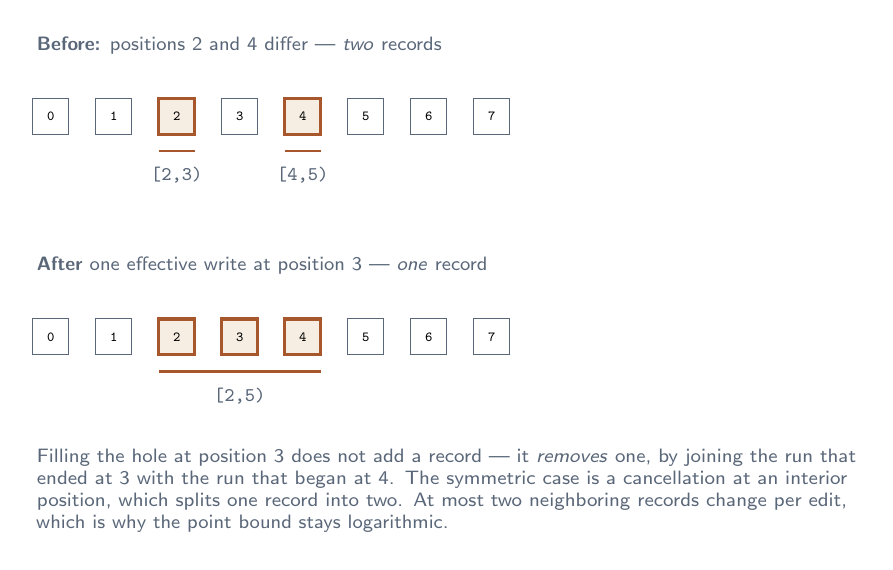
\begin{tikzpicture}[x=1mm,y=1mm]
  \node[d7label,anchor=west] at (-3,9)
    {\textbf{Before:} positions 2 and 4 differ --- \emph{two} records};
  \foreach \i in {0,1,3,5,6,7}
    {\node[d7cell] at ({8*\i},0) {\i};}
  \foreach \i in {2,4}
    {\node[d7cell,fill=d7sun,draw=d7copper,very thick] at ({8*\i},0) {\i};}
  \draw[d7copper,thick] (13.7,-4.4) -- (18.3,-4.4);
  \draw[d7copper,thick] (29.7,-4.4) -- (34.3,-4.4);
  \node[d7label,anchor=north] at (16,-5.2) {\texttt{[2,3)}};
  \node[d7label,anchor=north] at (32,-5.2) {\texttt{[4,5)}};

  \node[d7label,anchor=west] at (-3,-19)
    {\textbf{After} one effective write at position 3 --- \emph{one} record};
  \foreach \i in {0,1,5,6,7}
    {\node[d7cell] at ({8*\i},-28) {\i};}
  \foreach \i in {2,3,4}
    {\node[d7cell,fill=d7sun,draw=d7copper,very thick] at ({8*\i},-28) {\i};}
  \draw[d7copper,thick] (13.7,-32.4) -- (34.3,-32.4);
  \node[d7label,anchor=north] at (24,-33.2) {\texttt{[2,5)}};

  \node[d7label,anchor=north west,align=left,text width=104mm] at (-3,-41)
    {Filling the hole at position 3 does not add a record --- it \emph{removes}
     one, by joining the run that ended at 3 with the run that began at 4. The
     symmetric case is a cancellation at an interior position, which splits one
     record into two. At most two neighboring records change per edit, which is
     why the point bound stays logarithmic.};
\end{tikzpicture}
\caption{The maximal-run index. Run descriptors are stored as
\texttt{start} $\to$ \texttt{endExclusive} in a persistent ordered map, so
enumerating them is $\Theta(r)$ and locating the run containing a position is a
floor query.}
\label{fig:runindex}
\end{figure}

\subsection{The four transitions, and the local cases inside two of them}

An edit at position $i$ compares the incoming value with the current value
first, and then --- before allocating or publishing anything --- with the
checkpoint value. Only four transitions exist, and only two of them touch the
run index.

\needspace{11\baselineskip}
\begin{d7table}{0.31}
\toprule
\thead{Transition at position $i$} & \thead{What the run index does} \\
\midrule
relation-equal to the current value & Nothing. The receiver is returned. \\
clean $\to$ dirty & Insert $i$, joining whatever it now touches: join a run
ending at $i$ with one starting at $i+1$; extend the left run rightward; extend
the right run leftward; or create the singleton \code{[i, i+1)}. \\
dirty $\to$ dirty & Nothing. The record already covers $i$. \\
dirty $\to$ clean & Remove $i$ from its unique containing run: delete a
singleton record; trim its left edge; trim its right edge; or split it into two
records. \\
\bottomrule
\end{d7table}

\noindent
At most two neighboring records change, so a point edit is one RRB path copy
plus a constant number of logarithmic predecessor, successor, and update
operations on the run map: \bigoh{\log n} time and fresh nodes. If removing the
last dirty position empties the run index, the current root snaps back to the
checkpoint root exactly as the delta map's does, and the validator enforces it
--- a clean vector that has not been canonicalized is rejected.

\subsection{What the run index buys}

Two things, and they are different in kind.

The first is discovery. Enumerating run descriptors is $\Theta(r)$, which is
output-optimal because the answer has $r$ records. The baseline it improves on
is worst-case $\Theta(n)$: from two unindexed roots, an exact set of run
boundaries can require inspecting every position, because until a position is
examined its two values can be equal or unequal without changing anything
observed so far. The gap is unbounded --- one contiguous changed block gives
$k = n$ dirty positions and $r = 1$ run, and the focused suite pins that with a
clustered witness of 8{,}191 dirty positions represented by two descriptors.
Against an explicit point-delta index the unconditional statement is about
metadata rather than time: $\Theta(r)$ live records instead of $\Theta(k)$. A
linear coalescing scan over point records costs $\Theta(k)$, and the library is
candid that this is not a representation lower bound for every order-statistic
point index, and that a balanced Discrete Interval Encoding Tree in Erwig's
sense --- which is essentially what the run index is --- matches these bounds
exactly. No new interval algorithm is claimed.\index{DIET}

The second is the hunk operation, and it is the one that surprises. Accepting
one run splices that range of the current root over the checkpoint root;
reverting splices the checkpoint range back over the current root. Both are
composed from four RRB splits and two concatenations, so both cost
\bigoh{\log n} \emph{independently of the run's length} --- accepting a run of
one position and a run of a million positions cost the same --- and both invoke
the value relation zero times. The positions outside the interval keep both
roots untouched. When the selected run is the only run, the operation folds into
\code{Checkpoint} or \code{Rollback} and becomes a constant-time root exchange.

\begin{lstlisting}[language={[Sharp]C}]
var slab = PersistentRunDeltaVector<int>.CreateRange([0, 0, 0, 0, 0, 0, 0, 0]);

var edited = slab.SetItem(2, 7).SetItem(4, 9).SetItem(3, 8);

var dirty = edited.DirtyCount;      // 3
var runs  = edited.DirtyRunCount;   // 1 -- writing 3 joined [2,3) and [4,5)
var run   = edited.GetDirtyRunAt(0);// Start = 2, Length = 3

var kept    = edited.AcceptDirtyRunAt(0);         // checkpoint takes 7, 8, 9
var dropped = edited.RevertDirtyRunContaining(3); // current back to zeros
var split   = edited.ResetItem(3);                // interior: one run becomes two

// slab and edited remain valid and independently editable.
\end{lstlisting}

\begin{caveatbox}[Only the descriptors are run-sensitive]
Enumerating, hashing, serializing, or applying all the \emph{changed values} is
still $\Omega(k)$ for $k$ dirty positions, and the library says so rather than
letting the $\Theta(r)$ headline imply otherwise. Nor is the vector globally
optimal as a persistent array: Dietz's fully persistent arrays and Straka's
worst-case refinement beat these \bigoh{\log n} point operations outright. They
simply do not expose dirty-run semantics. The discovery result applies to the
declared RRB comparator family and to nothing wider. Starting from one $n$-element
version, $m$ retained effective point edits occupy \bigoh{n + m \log n}
worst-case total structural space; that history bound is not collapsed to
\bigoh{n}.
\end{caveatbox}

\section{The reference-identity invariant}

Both structures canonicalize, and the vector's version of the rule is strict in
a way that turns out to constrain the ports: a clean position must reuse its
\emph{exact} checkpoint cell, not an equal one. The validator states it as such
and fails a version in which a clean position's current and checkpoint entries
are distinct objects.\index{reference identity}

The rule earns its strictness by being load-bearing, and the cell is what makes
it hold. The RRB substrate recognizes a leaf no-op with its \emph{own} default
equality, while this collection decides dirtiness with a caller-supplied
relation --- two different relations judging the same write. Wrapping each value
in a private cell whose default equality \emph{is} reference identity reconciles
them: a genuine edit installs a fresh cell, a cancellation installs the
checkpoint's own cell, and the substrate can never quietly retain an
equal-but-different object on the reasoning that its own comparer saw no change.
Without that, a clean position could hold a value equal under one relation and
distinct under the other, the two roots would drift apart physically while
agreeing extensionally, and the canonicalization the run index depends on would
be defeated.

Stating the invariant is easy; making it \emph{testable} is where the languages
diverge, because in several of them the natural identity operator on the payload
types a test reaches for first is value equality. Python's \code{is} is true for
equal small integers, booleans, and interned strings. TypeScript's \code{===} is
value equality on numbers and interned strings. OCaml's \code{==} is value
equality on immediates. In each of those workspaces the run-delta vector boxes
every element in a private, identity-bearing cell so that the invariant has
something to be about. In Python and TypeScript there was no substrate rule to
defeat --- their leaf writers already short-circuit on identity rather than on
equality --- so the boxing exists purely to make the invariant observable, and
the ports say so. C\# uses the same device, a private sealed \code{Cell}
class whose default equality is reference equality by construction. Rust
replaces it with \code{Arc<T>} and \code{Arc::ptr\_eq}: the same reference
identity with one fewer allocation layer. Haskell has the hardest problem, since
pure code exposes no object identity at all, and solves it by giving each cell a
globally unique token drawn from an atomic counter through the
\code{unsafePerformIO}/\code{NOINLINE} device \code{Data.Unique} uses --- which
makes the identity test available to the \emph{pure} validator, with
\code{StableName} diagnostics confirming the same fact independently in the
tests.

\section{The relation that decides everything}

Both structures retain a value equality relation, and it is not a convenience.
It decides which writes are no-ops, and it decides when a delta cancels ---
which is to say it decides the observable change set. Two versions built from
identical operations under different relations are legitimately different
values, which is why the relation is retained on the instance rather than taken
as a static constraint.

Its precondition is that it be a genuine equivalence relation: reflexive,
symmetric, transitive, and stable for the lifetime of every version derived from
it. Reflexivity is the one that gets violated in practice, and it fails in the
most ordinary way imaginable.

\begin{caveatbox}[A non-reflexive relation corrupts the accounting silently]
IEEE floating point says \code{NaN != NaN}, so any relation that forwards to
primitive floating-point equality is not reflexive. Rewriting a position with
the identical \code{NaN} then fails the no-op test, the position is recorded as
dirty against a checkpoint value it is bit-identical to, and the phantom run
corrupts run counts, ranks, and the dirty count for every subsequent
operation.\index{NaN}

The reason this is worth a caveat box rather than a footnote is that
\emph{no internal validation can detect it}. The index remains perfectly
consistent with the relation it was given; the relation is simply not an
equivalence relation. The library states that limitation outright rather than
implying a validator that cannot exist.

The ports therefore defend at the type level or at the policy level. Rust
bounds its natural policy constructors on \code{Eq} rather than
\code{PartialEq}, so \code{f64} --- which is not \code{Eq} --- fails to
\emph{compile} against the natural policy instead of silently diverging, and
canonical \code{EqualityPolicy::reflexive\_ieee} constructors supply the
.NET-matching behavior for callers who do want floats.
Python's \code{natural\_value\_equality} consults identity first and
\code{reflexive\_ieee\_equality} collapses every \code{NaN} into one class.
OCaml's default relation is \code{compare x y = 0} rather than \code{( = )},
because on that toolchain \code{nan = nan} is false while \code{compare nan nan}
is zero. Kotlin needs no escape hatch at all: its natural policy is generic, so
it boxes and reaches \code{java.lang.Double.equals}, which compares raw bits and
\emph{is} reflexive on \code{NaN} --- the residual difference from .NET being
signed zero, which the boxed comparison separates and
\code{EqualityComparer<double>.Default} does not.

OCaml recovers a partial check the others do not attempt: its structural audit
rejects a version whose relation is observably non-reflexive \emph{at a clean
position}, where current and checkpoint are literally the same cell and the
relation must therefore answer true. That catches the cause, even though the
consequence at dirty positions stays invisible --- which is exactly the
condition the Rust port documents as undetectable.
\end{caveatbox}

Failure atomicity follows the same discipline in both structures: every policy
call happens before any successor is constructed, so a throwing relation or
comparer publishes nothing and leaves the receiver and every retained branch
intact. What cannot be undone is a side effect inside a callback, and the
documentation says that plainly rather than implying transactionality it does
not have.

\section{Where the ports differ}

The repository's cross-language parity work left these two structures unusually
well characterized, including in the places where the ports are not equal.

\begin{d7table}{0.30}
\toprule
\thead{Divergence} & \thead{Where, and why} \\
\midrule
Delta-map extremes &
\bigoh{1} in C\#, C\texttt{++}, Haskell, OCaml, Python, and TypeScript, where the
ordered substrate is a finger tree and \code{MinEntry}/\code{MaxEntry} are digit
reads. $\Theta(\log N)$ in C, Kotlin, and Rust, whose ordered cores cache
subtree sizes but no extremes, making an extreme a rank select like any other.
Each port documents its own. \\
Run-splice qualifier &
C\#, Rust, Python, and OCaml state the point edit and the run splice worst case
outright, their RRB and run-index substrates deferring nothing. TypeScript
splits the claim: the splice is worst case, the run-index write amortized
through its finger tree's concatenation. C\texttt{++} states every
run-index-routed operation amortized, because that substrate may force a pending
lazy spine on a read. \\
Change-enumeration setup &
C\#'s \code{GetChanges()} is a lazy iterator with $\Theta(1)$ setup; Rust's
\code{get\_changes} materializes, so setup is $\Theta(k)$. Full consumption is
$\Theta(k + 1)$ in both. \\
\bottomrule
\end{d7table}

\noindent
The run-splice row is a small monument to how that work proceeded. The reference
implementations originally documented those bounds as amortized --- a true
statement, but weaker than their eager code paths deliver. A freshly ported
workspace stated the worst-case bound instead, and under a governing principle
that says the stronger true statement wins, the C\# and Rust documentation was
raised to match the port rather than the port lowered to match the
reference.\index{complexity parity}


% ---------------------------------------------------------------------------
% Chapters: The Monotone-Action Heap; The Ancestral Connection Forest
% Fragment for durable7-data-structures.tex -- \input at the right place.
% ---------------------------------------------------------------------------

\chapter{The Monotone-Action Heap}
\label{ch:actions}

\motto{Rewriting every priority should not cost you every entry.}

\begin{specimen}[Specimen --- \code{PersistentMonotoneActionHeap}]
\index{PersistentMonotoneActionHeap@\texttt{PersistentMonotoneActionHeap}}%
\spec{Purpose}{Apply one order-preserving transformation to every priority currently in a heap, in constant time, without giving up meld, worst-case bounds, or persistence.}
\spec{Core}{The bootstrapped skew-binomial representation of \code{BrodalOkasakiHeap} (Brodal and Okasaki, \textit{JFP} 1996), with one immutable \emph{pending action} on every tree node and forest spine cell.}
\spec{Operations}{Insert, minimum, meld, and \code{TransformAll}: \bigoh{1} worst case. Delete-minimum: \bigoh{\log n} worst case. Enumeration and validation: $\Theta(n)$. Forking: \bigoh{1}.}
\spec{Algebra}{Identity, identity test, associative \code{Compose(outer, inner)} denoting \code{outer(inner(p))}, and \code{Apply} --- each \bigoh{1} over fixed-size actions, every action monotone for the retained comparer.}
\spec{Policies}{Trusted: no finite runtime check establishes associativity or monotonicity, so a policy that breaks its contract invalidates the semantics and the bounds together.}
\spec{Ports}{All nine.}
\end{specimen}

\noindent
A branchable scheduler holds a hundred thousand pending jobs in a persistent
heap, and a policy change arrives: nothing may run before Tuesday. Every
priority in the heap has to move up to that floor.

The ordinary way to do that is to take the heap apart and put it back together.
The Haskell \code{heaps} package's \code{Data.Heap} --- itself a persistent
Brodal--Okasaki heap, with the same worst-case \bigoh{1} insert, minimum, and
union and worst-case \bigoh{\log n} delete-minimum that this repository's
\code{BrodalOkasakiHeap} delivers (Chapter~\ref{ch:priority}) --- offers
\code{mapMonotonic} at \bigoh{n}, and that is an honest price for an arbitrary
promised-monotone function. Emulating the same change through this library's
own state-only heap costs the same: enumerate, transform, rebuild ---
$\Theta(n)$.

\code{PersistentMonotoneActionHeap<TElement, TPriority, TAction>} pays
\bigoh{1} instead, worst case, allocating \bigoh{1} new structure --- and it does
so without weakening any of the bounds it inherits. The trade that buys this is
narrow and worth stating up front: the transformation may not be an arbitrary
function. It must come from a fixed, closed family of actions that compose in
constant time and preserve the priority order. Under that restriction, and only
under it, transforming the whole heap becomes a single note written on the root.

\begin{asidebox}[The scope of the claim]
Recursively tagged heaps are, by construction, an equal-bound implementation of
this idea; the proposal for this structure says so explicitly. What is claimed
is the aggregate: a worst-case-optimal fully persistent meldable heap, a generic
action policy that may be \emph{non}-invertible, constant-time whole-heap
transformation with version-local temporal semantics, and exact priority
representatives under comparer-equivalent clamp boundaries. Tarjan's
\code{addtokeys} is the important ancestor here, and it is an invertible
translation --- which, as the next pages show, is a materially easier problem.
\end{asidebox}

\section{The algebra, and the one law that carries the structure}

The policy interface has four members and no others:

\begin{itemize}
\item an \term{identity} action;\index{action policy}
\item \code{IsIdentity}, which recognizes it;
\item \code{Compose(outer, inner)}, associative; and
\item \code{Apply}, which runs an action on one priority.
\end{itemize}

\noindent
The laws are the ones you would guess. Applying the identity returns the
priority unchanged; applying a composite equals applying the inner action and
then the outer one. Two further requirements are not laws about values but about
cost, and they are just as binding. Every operation above must be \bigoh{1}, and
every composed action must stay \emph{fixed size}. The second condition is the
one that quietly kills naive designs: storing a chain of pending transformations
instead of collapsing them would make \code{Minimum} linear in the number of
retained transforms, and the advertised bound would evaporate without a single
test failing.

The law that actually holds the structure together, though, is monotonicity:

\begin{contractbox}[The monotonicity requirement]
For every action $a$ and all priorities $p$, $q$ ordered by the heap's retained
comparer,
\[ p \leq q \;\Longrightarrow\; \mathrm{Apply}(a, p) \leq \mathrm{Apply}(a, q). \]
\end{contractbox}

Everything depends on this. A tag attached to a node is a promise about that
node \emph{and its entire subtree}: every priority underneath is logically the
stored value with the pending action applied. The heap property says that each
parent's priority is no greater than each child's. If the pending action can
reverse a single one of those relations --- if some parent/child pair with
$p \leq q$ becomes $a(p) > a(q)$ --- then attaching one tag has silently broken
the heap, everywhere below that node at once, and nothing in the operation that
attached it looked at those nodes to notice. A whole-heap transform is only
sound because a monotone action preserves \emph{every} existing order relation
simultaneously; that is precisely why \code{Minimum} may apply the root's tag and
return the same root without re-examining anything, and why melding, linking,
and splitting keep working on tagged components as if the tags were not there.

Negation is the obvious excluded case, and it is excluded for exactly this
reason. So is any permutation of the priority domain that reverses a pair.
Neither is repairable by cleverness in the heap; both require a rebuild, and the
structure does not pretend otherwise.

\section{Composition has a direction}

\begin{center}
\fbox{\parbox{0.86\linewidth}{\centering\vspace{2pt}
\code{Compose(outer, inner)} means: apply \emph{inner} first, \emph{outer}
second.\vspace{2pt}}}
\end{center}

\noindent
Equivalently, \code{Compose(outer, inner)} denotes \code{outer(inner(p))}. At
every site where a tag is pushed down or merged, the \emph{newer} action is the
outer one:\index{composition direction} a node already carrying a pending $b$
that receives a fresh $a$ ends up carrying \code{Compose(a, b)}, because $a$
arrived later and therefore runs last.

This deserves the box because getting it backwards is a bug that hides. Swap the
two arguments and the composite is still a member of the action family, and it
is still monotone --- so the heap remains perfectly well formed. Ranks are
untouched. Parents still compare no greater than children. The structural
validator, which checks rank encodings, logical heap order through every pending
action, and the count, passes without complaint. Only the \emph{values} are
wrong, and only for entries that happened to accumulate two or more
non-commuting actions. The C\texttt{++} port review treats this as a first-class
hazard and confirms the composition-direction case by mutation: the test fails
against a deliberately reversed kernel, which is the only evidence worth having
for a property this quiet. The same book-wide convention appears in the
range-update sequence's tag monoid (Chapter~\ref{ch:range}); the two structures
state the direction in the same words for the same reason.

\section{Where the tags live}

A version retains a root tree, a count, the comparer, and the policy. Two kinds
of cell carry pending actions, and both are load-bearing:

\begin{d7table}{0.26}
\toprule
\thead{Cell} & \thead{Tag scope} \\
\midrule
Tree node & The node and every descendant. A tree can be relinked as a unit, so
its action must travel with it. \\
Forest spine cell & Uniformly, every tree in that spine \emph{suffix} --- which
is what lets an action be pushed down one cell at a time without walking the
rest of the suffix. \\
\bottomrule
\end{d7table}

\noindent
Three logical views do all the work. \code{TagTree} and \code{TagForest}
compose a newer action onto a node or spine cell. \code{Expose} normalizes one
tree: it applies the node's pending action to that node's own priority and moves
the same action onto the child forest --- one new spine cell, not a traversal
--- leaving an identity-tagged node behind. Every structural consumer reaches
children through tag-composing accessors rather than through raw fields, so a
detached tail can never lose the action that governed it.

Two consequences follow. First, tags do not change ranks or forest shape, so the
skew-binomial rank encoding is preserved by tagging exactly as it stands; the
insert path exploits this by reading raw spine ranks to decide whether a link is
needed \emph{before} materializing any tagged tail node. Second, tags are pushed
down only at places where the underlying Brodal--Okasaki algorithm already
exposes a component --- which is why the ordinary bounds are not merely
preserved in spirit but unchanged: insert, minimum, and meld stay \bigoh{1}
worst case, and delete-minimum stays \bigoh{\log n} worst case, each counting the
\bigoh{1} policy calls and comparisons it performs.

\section{The clamp family, and why it is the interesting case}

\code{OrderClampPolicy<T>} ships one closed family:\index{OrderClamp@\texttt{OrderClamp}}
\code{AtLeast} (a floor), \code{AtMost} (a cap), \code{Between} (a validated
two-sided clamp, which rejects a lower bound comparing greater than the upper),
and \code{Constant}. A missing bound denotes an infinity. The identity is the
clamp with neither bound.

Clamp is the interesting family precisely because, unlike the familiar additive
heap offset, it is \emph{not invertible}. After flooring a heap's priorities at
zero, there is in general no raw priority you could assign to a later insertion
such that one flat normalization recovers the value the caller asked for. The
proposal's witness is small enough to check by hand. Take a heap holding
$-10$ and $100$, clamp it to $[0, 10]$, and then insert $50$. Draining must
yield $0$, $10$, $50$: the new entry never existed when the clamp happened.
Applying the old root's tag to the newcomer would produce $0$, $10$, $10$. And
in a second retained branch off the same clamped heap, inserting $-20$ must
yield $-20$, $0$, $10$ --- so there is no single flat clamp that could stand in
for the pair of histories. Recursive fixed-size tags are what close the
representation under the full operation set; a flat wrapper simply does not
implement this ADT.

Composition of two clamps must still be one clamp, in constant time. The rules
are worth reading closely, because three of the four are asymmetric:

\begin{d7table}{0.34}
\toprule
\thead{Case} & \thead{Result} \\
\midrule
Either side is the identity & The other side, unchanged. \\
The \emph{outer} is a constant & The outer constant. Nothing the inner action
did can survive a later constant function. \\
The \emph{inner} is a constant & A constant carrying the outer action applied to
the inner's value. \\
Disjoint bounds & A constant carrying the \emph{outer} boundary. Cap everything
at 5 and then floor at 10, and every output is 10. \\
Overlapping bounds & The intersection $[\max(iL, oL), \min(iU, oU)]$, keeping the
\emph{inner} representative when two boundary values compare equal. \\
\bottomrule
\end{d7table}

\noindent
Two of those rows encode a distinction that is easy to miss. Composition
produces an explicit \code{Constant} rather than the inclusive interval
$[k, k]$, and it keeps the older --- inner --- representative on tied
boundaries. Both choices exist for the same reason: a comparer may treat
distinct priority \emph{values} as equal. An inclusive $[k, k]$ clamp passes
through an input that compares equal to $k$, preserving that input's own
representative, whereas the constant function must return the exact $k$ the
caller supplied. So the family preserves exact sequential results, not merely
comparison equivalence --- which is a stronger promise than a heap has any
obligation to make, and is the kind of promise that only survives if someone
writes it down.

Because monotonicity is a property \emph{relative to a comparer},
\code{OrderClampPolicy} implements a second interface that names the exact
comparer object for which it is monotone, and heap creation adopts that comparer
and rejects any other. Melding likewise requires comparer and action-policy
object identity. These are not defensive gestures; a policy monotone for one
order is generally not monotone for another, and silently mixing the two would
reintroduce the failure that monotonicity exists to prevent.

\section{Temporal semantics: expose before you attach}

\code{TransformAll} transforms every priority \emph{present in this version}.
Entries inserted later are not retroactively transformed, and neither are
entries arriving through a later meld. That sentence is the whole reason the
structure is usable as a scheduling primitive: a floor imposed on Monday's
backlog must not silently apply to a job filed on Wednesday under the current
external priority scale.

The mechanism is one ordering rule, applied everywhere components with different
histories meet. \code{Insert} compares an untagged singleton against the
\emph{logical} root. If the singleton wins, it becomes a fresh identity-tagged
global root and the old tagged root becomes its child, carrying its own action
down with it. If the old root wins, it is \emph{exposed first} --- its pending
action pushed onto its own children --- and only then is the new singleton
skew-inserted into the resulting child forest, through an identity-tagged spine
cell (Figure~\ref{fig:actiontemporal}). \code{Meld}, \code{Link}, and
\code{SkewLink} follow the same rule: compare logical roots, expose only the
winner, attach the loser through an identity cell. Delete-minimum exposes the
global root, selects the least logical tree in its child forest, and exposes
that tree before splitting its fused children.

\begin{figure}[htbp]
\centering
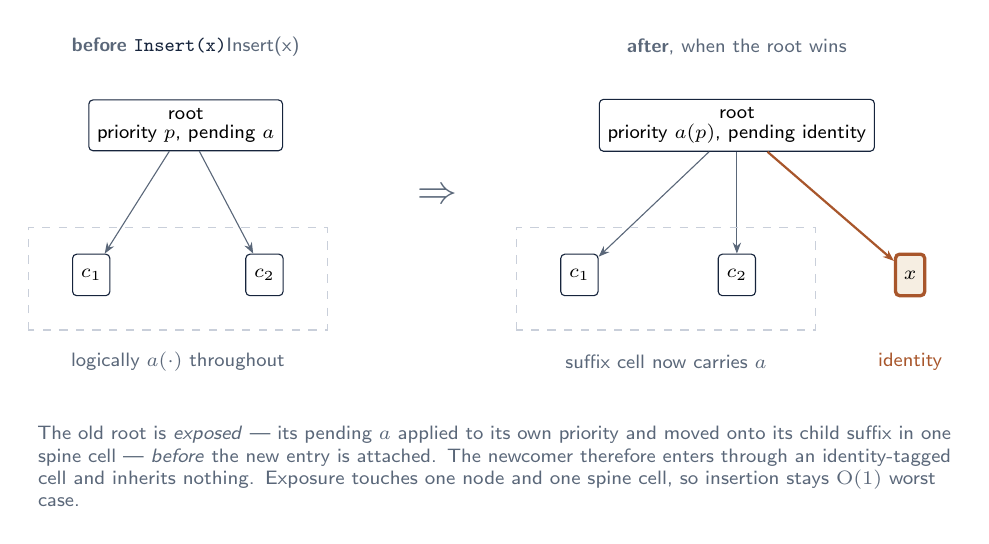
\begin{tikzpicture}[x=1mm,y=1mm]
  % --- before ---
  \node[d7label] at (-40,27) {\textbf{before} \code{Insert(x)}};
  \node[d7node,align=center] (r0) at (-40,17)
    {root\\[-1pt]{\scriptsize priority $p$, pending $a$}};
  \node[d7node] (c01) at (-52,-2) {$c_1$};
  \node[d7node] (c02) at (-30,-2) {$c_2$};
  \draw[d7edge] (r0) -- (c01);
  \draw[d7edge] (r0) -- (c02);
  \draw[d7rule,dashed] (-60,-9) rectangle (-22,4);
  \node[d7label] at (-41,-13) {logically $a(\cdot)$ throughout};

  \node[d7label] at (-8,8) {\Large$\Rightarrow$};

  % --- after ---
  \node[d7label] at (30,27) {\textbf{after}, when the root wins};
  \node[d7node,align=center] (r1) at (30,17)
    {root\\[-1pt]{\scriptsize priority $a(p)$, pending identity}};
  \node[d7node] (c11) at (10,-2) {$c_1$};
  \node[d7node] (c12) at (30,-2) {$c_2$};
  \node[d7newnode] (x) at (52,-2) {$x$};
  \draw[d7edge] (r1) -- (c11);
  \draw[d7edge] (r1) -- (c12);
  \draw[d7newedge] (r1) -- (x);
  \draw[d7rule,dashed] (2,-9) rectangle (40,4);
  \node[d7label] at (21,-13) {suffix cell now carries $a$};
  \node[d7label,text=d7copper] at (52,-13) {identity};

  \node[d7label,anchor=north west,align=left,text width=116mm] at (-60,-20)
    {The old root is \emph{exposed} --- its pending $a$ applied to its own
     priority and moved onto its child suffix in one spine cell --- \emph{before}
     the new entry is attached. The newcomer therefore enters through an
     identity-tagged cell and inherits nothing. Exposure touches one node and one
     spine cell, so insertion stays \bigoh{1} worst case.};
\end{tikzpicture}
\caption{Expose-before-attach. The rule is what makes ``every priority
\emph{currently} in this version'' a meaningful phrase rather than an
approximation.}
\label{fig:actiontemporal}
\end{figure}

Melding two independently transformed heaps is the case that shows the design
earning its keep. Continue the earlier example: a second heap holds $50$ and
$200$ and is independently clamped to $[60, 70]$. Melding it with the
$[0, 10]$-clamped heap must drain $0$, $10$, $60$, $70$. Losing the second
heap's tag would expose $50$ and $200$; leaking the first heap's tag into the
second would turn its entries into tens. Each operand keeps its own action
history until an ordinary structural operation exposes a component --- and the
meld itself remains \bigoh{1} worst case, with both operands still valid and
independently extendable afterwards.

\section{Where the guarantees stop}

\begin{caveatbox}[The honest limits]
Enumeration and \code{ValidateStructure} apply pending actions as they walk, so
both are $\Theta(n)$; the \bigoh{1} claim is about transformation, not about
reading everything.

Persistence does not make total history free. A single current version occupies
\bigoh{n}; starting from $n_0$ entries, $u$ retained updates use
\bigoh{n_0 + u \log N} worst-case total structural space for the maximum size
$N$ encountered --- a safe upper bound that is smaller for histories dominated
by constant-allocation updates.

The policy is trusted, and a throwing comparer or policy call publishes no
successor, leaving every existing version untouched --- but side effects the
callback performed cannot be rolled back.

There are no element handles, no decrease-key, no deletion by handle, and no
arbitrary heap mapping. Equal-priority tie order is unspecified. Payload
identity is preserved when priorities collapse, which is why payload and
priority are separate fields rather than one comparable value.
\end{caveatbox}

Two port notes are worth recording. Haskell takes the ordering and the action
family from a retained policy \emph{value} rather than a class constraint, which
keeps a fully drained heap usable --- but a record of functions has no identity
to compare, so unlike the managed ports it cannot reject operands built with
semantically different policies. Its documentation says so plainly, including the
consequence that melding two non-empty heaps adopts the left operand's policy
while an empty operand returns the other heap verbatim, so the surviving policy
depends on emptiness. And in OCaml this heap held, for a while, the only genuine
bootstrapped skew-binomial kernel in the workspace: when the complexity-parity
campaign found that workspace's plain \code{Brodal\_okasaki\_heap} storing its
elements in a list, the repair was to rebuild it as the untagged specialization
of the kernel its own action heap already contained.

\chapter{The Ancestral Connection Forest}
\label{ch:connectivity}

\motto{Not \emph{whether} two vertices are connected, but \emph{when} --- and
answered without consulting the history.}

\begin{specimen}[Specimen --- \code{PersistentAncestralConnectionForest}]
\index{PersistentAncestralConnectionForest@\texttt{PersistentAncestralConnectionForest}}%
\spec{Purpose}{Persistent, branching, insertion-only connectivity over a fixed integer vertex universe, plus one query ordinary union-find cannot answer: at which ancestor version did two vertices first become connected?}
\spec{Core}{A union-by-size parent forest stored sparsely in a CHAMP map, with every union edge labelled by the version that created it.}
\spec{Operations}{\code{Find}, \code{Connected}, \code{GetComponentSize}, \code{Link}, and \code{FirstConnected}: \bigoh{w \log n} worst case, for bounded CHAMP path cost $w$. \code{Create} and \code{ComponentCount}: \bigoh{1}. Forking: \bigoh{1}.}
\spec{Complexity}{\code{FirstConnected} costs exactly one connectivity query and is independent of history depth. A black-box persistent disjoint-set forest needs \bigoh{w \log n \log(K+2)} for $K$ successful unions on the queried lineage.}
\spec{Limits}{No deletion, no confluent merge of sibling versions, no retroactive update, no path compression, and no semantic guarantee on representative choice.}
\spec{Ports}{All nine.}
\end{specimen}

\noindent
Union-find answers ``are $x$ and $y$ connected?'' A persistent union-find answers
it per version, which is already useful: retain a version, fork it, ask each
branch separately. But there is a question just past that boundary which the
persistent version still cannot answer without brute force. Given a version $v$
and two vertices, \emph{which ancestor version of $v$ first put them in the same
component?}

The brute-force answer is a search. Connectivity along a lineage is monotone ---
once connected, always connected, since edges are only added --- so the versions
on the root-to-$v$ path split into a disconnected prefix and a connected suffix,
and binary search finds the boundary. The strongest form of that comparator
keeps an append-only index of only the successful-union versions and probes
$\log(K + 2)$ of them, where $K$ is the number of successful unions on the
lineage. Since $K$ can be $n - 1$, that is a full logarithmic factor above the
cost of a single connectivity query --- \bigoh{\log^2 n} against \bigoh{\log n}
in the CHAMP specialization, once the bounded trie factor is folded in.

\code{PersistentAncestralConnectionForest} answers the question at the price of
one connectivity query, and --- this is the part worth dwelling on --- it never
looks at the version history at all.

\section{The mechanism: an edge remembers its own birthday}

Each successful \code{Link} does one thing beyond ordinary union by size: it
labels the single new root-parent edge with the child version that created it.
Nothing else is recorded. There is no per-version snapshot, no event log, no
index over the lineage.

The query then works entirely inside the queried version's own parent forest.
Walk from each vertex to its root, collecting the edge labels on the way. If the
two roots differ, the vertices are disconnected and the answer is nothing. If
they agree, delete the shared rootward suffix of the two paths --- what remains
is exactly the two paths strictly below their forest lowest common ancestor ---
and return the \emph{latest} label among those remaining edges
(Figure~\ref{fig:firstconnected}).

\begin{figure}[htbp]
\centering
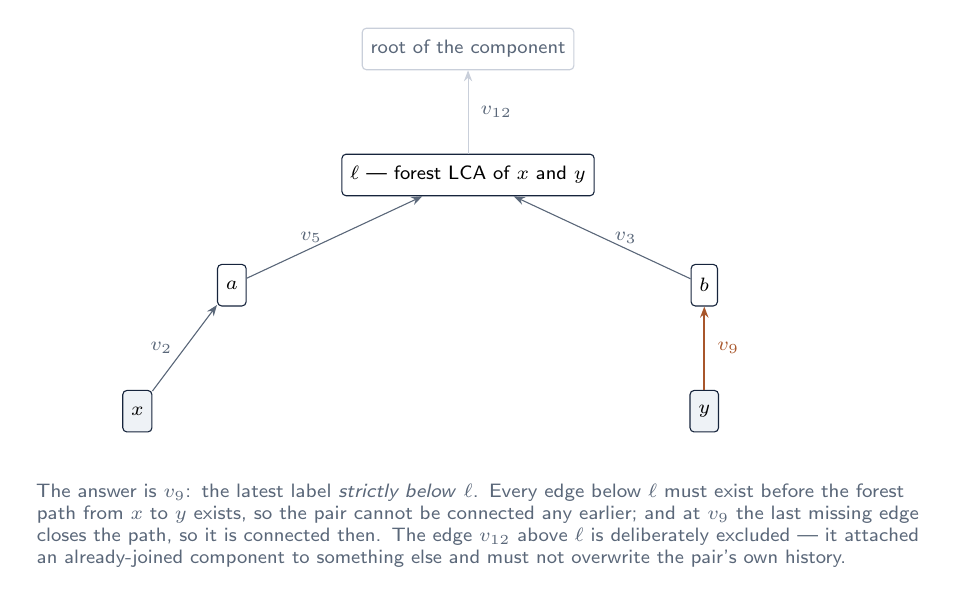
\begin{tikzpicture}[x=1mm,y=1mm]
  \node[d7ghost] (root) at (0,34) {root of the component};
  \node[d7node]  (l)    at (0,18) {$\ell$ --- forest LCA of $x$ and $y$};
  \node[d7node]  (a)    at (-30,4) {$a$};
  \node[d7node]  (b)    at (30,4) {$b$};
  \node[d7leafnode] (x) at (-42,-12) {$x$};
  \node[d7leafnode] (y) at (30,-12) {$y$};

  \draw[d7edge] (x) -- node[d7label,left=1pt] {$v_2$} (a);
  \draw[d7edge] (a) -- node[d7label,left=1pt] {$v_5$} (l);
  \draw[d7newedge] (y) -- node[d7label,right=1pt,text=d7copper] {$v_9$} (b);
  \draw[d7edge] (b) -- node[d7label,right=1pt] {$v_3$} (l);
  \draw[d7edge,draw=d7rule] (l) -- node[d7label,right=1pt] {$v_{12}$} (root);

  \node[d7label,anchor=north west,align=left,text width=112mm] at (-56,-20)
    {The answer is $v_9$: the latest label \emph{strictly below} $\ell$. Every
     edge below $\ell$ must exist before the forest path from $x$ to $y$ exists,
     so the pair cannot be connected any earlier; and at $v_9$ the last missing
     edge closes the path, so it is connected then. The edge $v_{12}$ above
     $\ell$ is deliberately excluded --- it attached an already-joined component
     to something else and must not overwrite the pair's own history.};
\end{tikzpicture}
\caption{\code{FirstConnected}. Two parent-path walks and a maximum; no version
is ever visited.}
\label{fig:firstconnected}
\end{figure}

Why is that the right answer, and why does it need no history scan? The argument
rests on a small fact about how union edges accumulate. When a root becomes a
child, both endpoints were roots an instant earlier, so every edge already below
the losing root was created strictly earlier --- and any edge later placed above
the winner is created strictly later. Labels therefore \emph{strictly increase}
toward the root along any path in any version's forest. Given that, the edges
below the pair's lowest common ancestor are exactly the edges whose existence
the connection required, and the last of them to appear is the moment the
connection happened. Everything above the ancestor is later history that both
vertices now share --- it moved them together, never joined them.

So the version history is not consulted because the answer is not stored in the
history. It is stored, distributed, one label at a time, in the shape of the
forest the queried version is already holding. Reading it costs the same two
root walks that any connectivity query costs: \bigoh{w \log n} worst case, with
\bigoh{\log n} transient path space, and --- worth stating twice --- independent
of how deep the history is.

\begin{caveatbox}[Why a query must not shorten the path]
Path compression, the reflex of every ephemeral union-find implementation, is
excluded here.\index{path compression} There are two reasons, and the second is
the load-bearing one.

The mechanical reason is that compression is a \emph{write performed by a read}.
In a structure whose queries must not disturb versions other readers hold, a
find cannot rewrite shared parent cells; it could only publish a new version,
which is not what a query is.

The semantic reason is that compression destroys the very boundary
\code{FirstConnected} reads. Union $a$ with $b$ at $t_1$, $c$ with $d$ at $t_2$,
join the two components at $t_3$, then compress $a$ and $b$ straight to the
final root. The correct answer for the pair $(a, b)$ is still $t_1$; but if the
compressed edges carry the maximum label they skipped, both paths now report
$t_3$, and the original lowest common ancestor --- the whole basis of the answer
--- has vanished. Richer summaries could preserve selected history queries, but
they are a different design and would owe a new proof.

The price of the exclusion is stated rather than hidden: bounds here are
worst-case logarithmic in component size, not the inverse-Ackermann amortized
bound an ephemeral union-find enjoys.
\end{caveatbox}

\section{Union by size, and the ceiling it alone guarantees}

With compression gone, the entire height argument rests on union by size. The
larger component's root wins; on a tie, the first endpoint's root stays the
representative, which makes results deterministic without touching the proof.
Every time a vertex's distance to its root grows by one, the component
containing it has at least doubled, and no component exceeds $n$ --- so every
parent path in every version has at most $\lfloor \log_2 n \rfloor$ edges. The
structural validator enforces exactly that number as a hard ceiling rather than
a comfortable approximation.

Persistence does not weaken the argument, because it applies independently to
the one forest each queried version selects. Nor can a sibling branch's update
contaminate a query: path copying gives siblings different roots at their
changed paths and shared immutable nodes everywhere else, so every cell and
every label a query observes belongs to the queried version or one of its
ancestors. Labels are compared only within a lineage, and a version's depth is
meaningful only against its own ancestors --- a sibling allocated later is not a
later state of this branch.

\section{What ``branching'' means here}

Every \code{Link} produces a distinct child version. That includes a redundant
one: linking two vertices already in the same component still yields a new
version token, which shares the complete connectivity index unchanged and adds
\bigoh{1} space. The parent is untouched, remains valid, and can be extended
again in a different direction. That is the entire content of the word
``branching'': the version graph is a tree, not a line, and old versions are not
merely readable but independently queryable and independently extendable.

Version identity is reference identity in the reference port, so two sibling
versions at equal depth are different versions even though their depths match.
Rust reproduces this with pointer identity behind a shared handle. Haskell
diverges deliberately and documents it: a version there is an ordinary immutable
value whose identity is structural, recording its link endpoints so that equal-depth
siblings stay distinct --- with the visible consequence, asserted in its test
suite rather than hidden, that two versions built by genuinely identical
operations from the same parent are one value.

The sparse representation is what keeps all this cheap. An absent cell means
``singleton root'', so a million-vertex forest allocates nothing per vertex and
\code{Create} is \bigoh{1} for any universe size. A stored root is therefore
always non-singleton, and it caches its component's size --- which is why
\code{GetComponentSize} is one root walk plus a cached read, at the same cost as
\code{Find}. A successful \code{Link} allocates \bigoh{w} new CHAMP nodes; a
redundant one allocates only its version wrapper and token.

\section{The path factor, and a guarantee that was strengthened}

\bigoh{w \log n} has two factors, and the second one has a story.

The CHAMP path cost $w$ is bounded by the number of trie levels a hash can
address --- at most seven for a 32-bit hash (Chapter~\ref{ch:champ}). For a
general CHAMP with arbitrary user keys, that per-level cost is only
\emph{expected} constant, because distinct keys can share a hash by pigeonhole
and a collision bucket must then be scanned. Here the keys are vertices from a
fixed integer universe, and distinct integers can be given distinct hashes ---
so the bound is unconditional, and the whole operation cost is worst case in
both factors.

Seven of the nine ports had that property from the start. Two --- Rust and
Haskell --- did not: each had reached for a general-purpose hasher whose output
was truncated, so distinct vertices could in principle collide and the honest
statement was ``expected''. The complexity-parity campaign of August 2026 treated
that as a violation rather than a documentation matter, and both were fixed by
pinning an injective 32-bit vertex hash --- MurmurHash3's \code{fmix32}
bijection, every step invertible modulo $2^{32}$ --- so that no collision bucket
can ever hold two distinct vertices. Haskell additionally caps its universe at
$2^{31} - 1$, the universe its siblings already had, because no 32-bit hash is
injective over a larger domain; \code{create} now rejects one, and the cap is
load-bearing rather than cosmetic. Both ports carry an inverse round-trip test
exhibiting the bijection.

The episode is a small, clean example of the campaign's governing rule at work.
The easy resolution --- write ``expected'' in two ports' documentation and move
on --- was available and would have been perfectly truthful. It was rejected
because a probabilistic guarantee and a worst-case guarantee are different
promises, and the library's claim is that the same structure delivers the same
bound in every language. Strengthening the code was cheaper than explaining the
divergence forever.

\section{Where the guarantees stop}

\begin{caveatbox}[Deliberate non-goals]
Edges can be added, never removed. After deletion, connectivity is no longer
monotone along a lineage and the whole first-connected question would need
redefining.

There is no confluent merge of sibling versions, no retroactive update of an
existing version, and no reconciliation across branches. \code{FirstConnected} is
defined only relative to one version's ancestor chain; it never returns a version
from another branch.

The structure returns the first connectivity \emph{event}, not a shortest path,
an original edge witness, bridge information, or an explanation. Representatives
returned by \code{Find} are implementation artifacts offered for interoperability;
the same component is not promised the same representative in sibling versions.

Version tokens retain their parent chains, so a deep history stays reachable from
any live version at \bigoh{\text{depth}} token space --- a cost per \code{Link},
not per successful union.

Finally, the comparison this structure wins is the \emph{online, branching} one.
A sealed linear history can be preprocessed into a component tree with \bigoh{1}
lowest-common-ancestor queries, and no superiority is claimed in that model.
\end{caveatbox}


% ===========================================================================
%  PART VI -- AUTHENTICATED
% ===========================================================================
\part{Authenticated Collections}
\label{part:authenticated}

\chapter{The Merkle Search Tree}
\label{ch:mst}

\motto{Structural sharing works across versions. Content addressing works across
machines.}

\begin{specimen}[Specimen --- \code{MerkleSearchTree}]
\index{MerkleSearchTree@\texttt{MerkleSearchTree}}%
\spec{Purpose}{An ordered, content-addressed persistent map whose root digest names the entire collection, so two processes that agree on a digest agree on every entry.}
\spec{Core}{A $B=16$ wide tree in which each key's layer is derived from the count of leading zero nibbles of its SHA-256 digest --- a geometric distribution --- so the shape is independent of insertion order.}
\spec{Identity}{Policy \code{mst-sha256-b16-v2}: a versioned semantic id, comparer semantics, canonical per-type codecs, and a SHA-256 domain digest.}
\spec{Wire}{The canonical \code{MST2} block format --- byte-identical across all nine ports.}
\spec{Order}{Policy comparer order, with range enumeration.}
\spec{Ports}{All nine, wire-compatible.}
\end{specimen}

\noindent
Everything up to this point exploits sharing \emph{within a process}. Two
versions of a persistent map diff cheaply because they share pointers, and
pointers do not survive a network. If the two collections you want to compare
live in different processes --- or on different machines, or were built a week
apart by unrelated code --- pointer identity tells you nothing and you are back
to comparing everything.

Content addressing fixes this by making the \emph{name} of a subtree a function
of its contents.\index{content addressing} Give every node a digest of what it holds, including the digests
of its children, and equal digests prove equal subtrees no matter who built them
or when. That is the Merkle idea, and applying it to an ordered map gives
the structure behind AT Protocol repositories (Bluesky) and Dolt's versioned SQL
tables.

\section{Shape from hashes, not from history}

A Merkle tree is only useful if equal contents produce equal digests, and that
requires equal contents to produce the \emph{same shape}. An ordinary B-tree
fails this immediately: insert the same entries in a different order and you get
a different --- equally valid --- tree.

Auvolat and Taïani's Merkle search trees (SRDS 2019) fix the shape by deriving
it from the data. Hash each key; count its leading zero nibbles; that count is
the key's \term{layer}.\index{Merkle search tree!layers} Since each additional zero nibble is a 1-in-16 event,
layers follow a geometric distribution with $B = 16$, which is exactly the
branching behavior a B-tree wants --- but assigned by the hash function rather
than by insertion history (Figure~\ref{fig:mst}).

\begin{figure}[htbp]
\centering
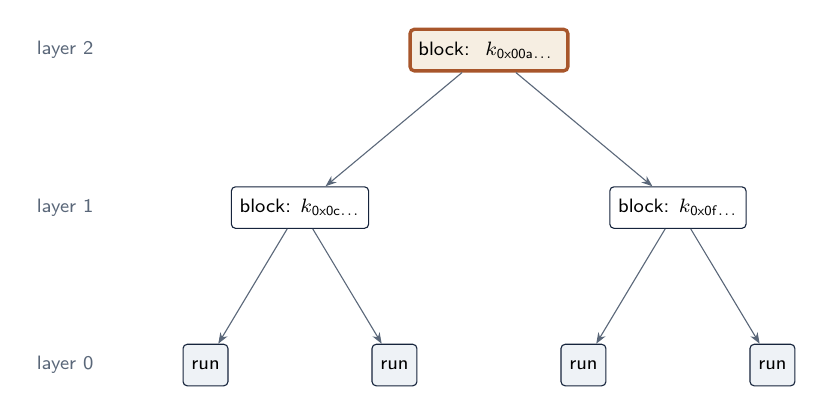
\begin{tikzpicture}[x=1mm,y=1mm]
  \node[d7label,anchor=east] at (-9,10) {layer 2};
  \node[d7newnode] (top) at (40,10) {block: $\;k_{\mathsf{0x00a\ldots}}\;$};
  \node[d7label,anchor=east] at (-9,-10) {layer 1};
  \node[d7node] (m1) at (16,-10) {block: $k_{\mathsf{0x0c\ldots}}$};
  \node[d7node] (m2) at (64,-10) {block: $k_{\mathsf{0x0f\ldots}}$};
  \node[d7label,anchor=east] at (-9,-30) {layer 0};
  \node[d7leafnode] (l1) at (4,-30)  {\scriptsize run};
  \node[d7leafnode] (l2) at (28,-30) {\scriptsize run};
  \node[d7leafnode] (l3) at (52,-30) {\scriptsize run};
  \node[d7leafnode] (l4) at (76,-30) {\scriptsize run};
  \draw[d7edge] (top) -- (m1); \draw[d7edge] (top) -- (m2);
  \draw[d7edge] (m1) -- (l1);  \draw[d7edge] (m1) -- (l2);
  \draw[d7edge] (m2) -- (l3);  \draw[d7edge] (m2) -- (l4);
\end{tikzpicture}
\caption{Layer assignment in a Merkle search tree. A key's layer is the number
of leading zero nibbles of its SHA-256 digest; one block holds each consecutive
same-layer run, and that block's digest covers the policy domain, its entries,
its subtree count, and its child digests. Because the shape comes from the
hashes, two processes that insert the same entries in different orders build the
same tree and compute the same root digest.}
\label{fig:mst}
\end{figure}

One block holds each consecutive run of same-layer keys, and each block's
\code{MST2} bytes cover the policy domain, its entries, its subtree count, and
its child digests. The root digest therefore names the whole collection.

\begin{asidebox}[Prolly trees, the convergent cousin]
Probabilistic B-trees --- ``prolly trees'', from Noms around 2016 and now Dolt
--- reach the same destination by a different route: instead of hashing each key
to a layer, they run a rolling hash over the entry stream and place a node
boundary wherever it crosses a threshold. This is \term{content-defined
chunking}, the same technique that powers \code{rsync}-style deduplication.
Both designs produce uniquely represented, content-addressed, history-independent
search trees; Durable7 implements the Merkle search tree variant.
\end{asidebox}

\section{Two prerequisites, taken seriously}

The repository treats content addressing as a capability that must be
\emph{earned} by satisfying two conditions, and records them as mandatory for
any future content-addressed family.

\begin{contractbox}[Prerequisite 1 --- pinned deterministic hashing]
Default string hashing on .NET is randomized per process. That is a fine defense
against hash-flooding and completely fatal for cross-process addressing. A
Merkle policy therefore binds a \emph{versioned semantic id}, canonical codecs,
comparer semantics, and a SHA-256 domain digest. The policy id versions the
application's comparer semantics: if you change what ``equal'' means, you change
the id, and old digests stop colliding with new ones by construction.
\end{contractbox}

\begin{contractbox}[Prerequisite 2 --- canonical serialization]
A digest is only as canonical as the bytes it hashes. A strict versioned codec
must \emph{encode and decode}, and its decoder must accept exactly one canonical
encoding while rejecting malformed, non-canonical, and trailing input. Codec ids
end in \code{-v} followed by decimal digits. The built-ins cover integers,
nullable strings, nullable byte arrays, and GUIDs.

Do not use a codec whose output depends on process-randomized hashes, culture,
object identity, ambient serialization settings, or mutable state. Every one of
those turns a content address into a lie.
\end{contractbox}

\begin{lstlisting}[language={[Sharp]C}]
var policy = MerkleSearchTreePolicy<int, string?>.Create(
    "document-index-v1",
    Comparer<int>.Default,
    MerkleCodecs.Int32,
    MerkleCodecs.Utf8String);

var baseline = MerkleSearchTree<int, string?>.Create(policy)
    .SetItem(10, "ten").SetItem(20, "twenty");
var updated  = baseline.SetItem(20, "TWENTY").SetItem(30, "thirty");

MerkleDigest address = updated.RootHash;

foreach (var (key, value) in updated.EnumerateRange(15, 30))
    Console.WriteLine($"{key}: {value}");
\end{lstlisting}

Recreate the same policy id, comparer semantics, codec ids, and logical entries
in any other language, and you get the same block graph and the same root
address. That is not an aspiration in this repository --- golden wire vectors are
shared test data, and a tree built in Rust verifies against a proof produced in
TypeScript.

\begin{caveatbox}[Diff is not free just because digests exist]
Equal block digests prune whole regions, and in-process \code{Diff} exploits
that. But a topology-changing edit can move a block separator, and when it does,
the implementation honestly falls back to ordered subtree comparison rather than
pretending the digest pruning still applies. The shipped API therefore does
\emph{not} promise \bigoh{\text{key divergence}} for every diff. Block
synchronization --- Chapter~\ref{ch:merkleops} --- is the divergence-oriented
path, and it is the right tool when the two trees live in different processes.
\end{caveatbox}

\chapter{Blocks, Proofs, Synchronization, and Merge}
\label{ch:merkleops}

\motto{The tree is the easy half. Not trusting the network is the other half.}

\noindent
A content-addressed collection is only interesting if it can leave the process.
This chapter covers the tier that lets it: storing blocks, moving them,
verifying them without trust, proving individual claims about them, and merging
two divergent descendants of a common ancestor.

Everything here ships in all nine languages with byte-identical wire behavior.

\section{Blocks and stores}

A \term{block} is one immutable node's canonical bytes, addressed by its digest.\index{block}
A \term{store} is a mapping from digest to block --- the persistence boundary.
The library's in-memory implementations are concurrent (an \code{RLock} in
Python, a shared mutex in C\texttt{++}, a synchronized three-state store in C),
and every store operation is atomic with respect to publication.

\begin{lstlisting}[language={[Sharp]C}]
var store = new InMemoryMerkleBlockStore();
int blocksAdded = updated.Save(store);

var loaded = MerkleSearchTree<int, string?>.Load(
    updated.RootHash, policy, store);
\end{lstlisting}

The critical property of \code{Load} is what it refuses to assume.

\begin{contractbox}[Load never trusts the store]
Loading recomputes every block digest, strictly decodes \emph{and re-encodes}
every entry to confirm canonicity, follows and validates every child reference,
checks the result against the expected root, and applies a finite verification
budget throughout. A store that returns tampered, malformed, non-canonical, or
merely inconsistent blocks produces an error, not a tree.

The re-encode step is the one people skip. Decoding alone proves the bytes are
\emph{parseable}; re-encoding and comparing proves they are \emph{canonical},
which is what the digest actually claims.
\end{contractbox}

\section{Packs, and the transport boundary}

A \term{pack} is a set of blocks prepared for transport.\index{pack} A \emph{complete} pack
is self-contained. A \emph{partial} pack can be completed from blocks the
destination already holds --- which is the common case, since two replicas of a
slowly changing tree share almost everything.

\begin{lstlisting}[language={[Sharp]C}]
MerkleBlockPack outbound = updated.ExportPack();

var replica = MerkleSearchTree<int, string?>.Import(
    outbound, policy, replicaStore);

Console.WriteLine(replica.RootHash == updated.RootHash);  // True
\end{lstlisting}

\code{Import} verifies every supplied block \emph{and} the requested root closure
before it performs destination conflict preflight, and it commits nothing until
all of that succeeds. A rejected import leaves the destination store exactly as
it was.

\section{Seven budgets}

Verification of untrusted input is where authenticated data structures go wrong,
and the failure mode is rarely a wrong answer --- it is resource exhaustion. A
malicious pack can be a decompression bomb, a cycle, a pathologically deep
closure, or a codec that allocates a gigabyte from four bytes.

\begin{contractbox}[Bounded verification]
Every port enforces \emph{seven} positive finite budgets during verification, and
the ordering of checks is itself part of the contract: query and proof-shape
limits run \emph{before} verifier allocation, hashing, or codec work. A malformed
request is rejected before it can cost anything.

Local proof and synchronization construction consumes a read-only trusted
topology view rather than applying network budgets or re-decoding values that are
already retained. The budgets exist for the trust boundary, and they are applied
at the trust boundary.
\end{contractbox}

\section{Proofs}

A proof lets a party who does \emph{not} have the tree verify a claim about it,
given only the root digest.\index{proof} The canonical \code{MSP2} format carries three kinds:

\begin{description}
\item[Membership] --- this key maps to this value in the tree named by this
digest.
\item[Non-membership] --- this key is \emph{absent} from that tree. This is the
harder and more valuable direction, and it works because the tree is ordered: the
proof exhibits the adjacent entries that would bracket the key, and the structure
guarantees nothing can hide between them.
\item[Range] --- these are exactly the entries between these bounds, with
nothing omitted.
\end{description}

Proof verification fixes query, shape, and envelope precedence before any decoder
or codec work runs, and tampering with any part of a proof --- the claimed value,
a sibling digest, the envelope --- produces a rejection rather than a wrong
answer. The test suites verify this adversarially rather than by inspection.

\section{Synchronization}

Synchronization answers: \emph{I have root $A$, you have root $B$, send me what I
am missing.} The mechanism is a frontier walk.\index{synchronization} Compare digests from the root
down; wherever they agree, an entire region is already shared and the walk stops;
wherever they differ, descend. The blocks the destination lacks form the
frontier, and the resulting sync pack is closure-pruned so that nothing already
present is retransmitted.

The walk is iterative rather than recursive --- a hostile tree should not be able
to overflow a stack --- and repair is likewise iterative, so a partially
populated store converges over successive rounds rather than requiring a
complete restart.

\section{Three-way merge}

The final operation is the one that turns an authenticated map into a version
control system: given a common ancestor and two descendants, produce a merged
tree.\index{three-way merge}

\begin{contractbox}[Merge obligations]
The merge is typed and \emph{present-null aware}: a key that was deleted in one
branch and a key whose merged value is present-and-null are different outcomes,
and the API distinguishes them rather than collapsing both into ``no value''.

A merged tree with unresolved conflicts is never published. Conflict detection
completes before any publication, so a caller either receives a complete merged
tree or receives the conflicts --- never a tree that is silently missing the
contested keys.
\end{contractbox}

That refusal to publish partial results is the same failure-atomicity rule from
Chapter~\ref{ch:contract}, applied where the stakes are highest. A partially
merged authenticated tree would still have a valid root digest, which means it
would be indistinguishable from a correct one --- a wrong answer that carries a
proof of its own correctness. The only safe design is to not produce it.

\begin{asidebox}[What this replaced]
An earlier design sketch in the repository proposed a \code{MerkleHamt}: content
addressing over the \emph{unordered} hash trie. It remains deferred. The Merkle
search tree is its ordered sibling and subsumes most of its uses while adding
range queries and range synchronization --- neither of which an unordered trie
can offer. Should \code{MerkleHamt} ever be revived, it must reuse equally
explicit hashing, encoding, verification-budget, and trust-boundary contracts;
the prerequisites are not negotiable per family.
\end{asidebox}

% ===========================================================================
%  PART VI -- CURSORS
% ===========================================================================
\part{Navigation}
\label{part:navigation}

\chapter{Cursors}
\label{ch:cursors}

\motto{A position that remembers which version it belongs to.}

\noindent
Persistent collections are excellent at whole-collection operations and
awkward at local editing. Inserting one character at position 4{,}000 of a rope
is a logarithmic descent; inserting sixteen characters one at a time is sixteen
logarithmic descents, and every one of them re-walks the same path.

A cursor fixes this by being what an iterator is not: an immutable value that
owns one collection version \emph{and} a position within it, from which both
navigation and editing are cheap and which can be retained and branched like any
other persistent value.\index{cursor}

\begin{contractbox}[What a cursor is, and is not]
Every initialized cursor owns or retains one immutable logical version and a
valid gap, rank, or measure boundary. Navigation returns a cursor over the
\emph{same} version. Editing returns a cursor over \emph{one new} version and
never changes the receiver, a retained ancestor, or a sibling branch. Snapshot
is non-consuming.

A cursor is not a detachable position, a mutable iterator, a builder, a
transient, a bookmark, a rebase operation, or a live concurrent view. There is
no implicit redirection to a later version and no cross-version application.
\end{contractbox}

\section{Gap semantics}

A positional cursor denotes a \emph{boundary}, not an element --- one of the
$n+1$ gaps in a sequence of length $n$ (Figure~\ref{fig:gap}).\index{cursor!gap semantics} This is the same
model a text editor's caret uses, and it is chosen for the same reason: an
insertion point between two elements is a first-class thing, and a cursor that
denoted an element could not represent ``before everything'' and ``after
everything'' without special cases.

\begin{figure}[htbp]
\centering
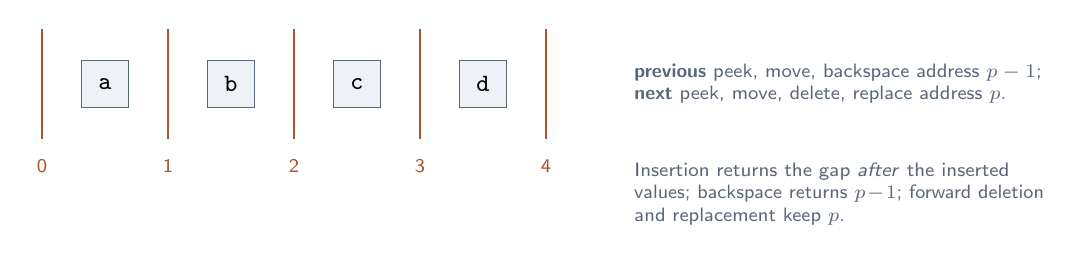
\begin{tikzpicture}[x=1mm,y=1mm]
  \foreach \i/\c in {0/a,1/b,2/c,3/d}
    {\node[d7cell, minimum width=17pt, minimum height=17pt, fill=d7mist,
           font=\ttfamily\small] at (12+\i*16,0) {\c};}
  \foreach \i in {0,1,2,3,4}
    {\draw[d7copper,thick] (4+\i*16,-7) -- (4+\i*16,7);
     \node[d7label,below=4pt,text=d7copper] at (4+\i*16,-7) {\i};}
  \node[d7label,anchor=west,text width=52mm,align=left] at (78,0)
    {\textbf{previous} peek, move, backspace address $p-1$;\\
     \textbf{next} peek, move, delete, replace address $p$.};
  \node[d7label,anchor=west,text width=52mm,align=left] at (78,-14)
    {Insertion returns the gap \emph{after} the inserted values; backspace
     returns $p-1$; forward deletion and replacement keep $p$.};
\end{tikzpicture}
\caption{Gap semantics. Empty, start, and end gaps are ordinary first-class
states rather than special cases.}
\label{fig:gap}
\end{figure}

Ordered cursors use the analogous idea over comparer order: the gap before the
next ordered candidate. A lower-bound miss leaves a \emph{usable} cursor rather
than an error, exact search carries a separate hit discriminator, and an edit
validates that the key or value actually belongs at the current gap. Nested
Ordered multimap cursors keep group and value positions explicit rather than
inventing a private flattened order that would not correspond to anything the
collection promises.

\section{Which families have one}

Not every collection has a meaningful ``next''. The library's rule is that a
cursor requires a stable \emph{semantic} neighbor axis, and hash traversal order
is not one.

\begin{d7table}{0.30}
\toprule
\thead{Family group} & \thead{Semantic axis} \\
\midrule
Patricia integer maps and sets & Ascending signed 32/64-bit key order, with rank
gaps. \\
Measured sequences, deques, reversible deques, RRB vectors, range-update
sequences, ropes and text & Position, or an ordered measure boundary. Text units
remain language-local. \\
Sorted bags, sets, and maps; canonical sorted sets; priority search queues;
interval trees and maps; chunked bit sets & Comparer order, interval order, key
order, or population-rank gaps, as owned by the family. \\
Neutral Ordered sets, maps, multimaps & Explicit position; the multimap
additionally exposes nested group and value positions. \\
Merkle search trees & Policy comparer order, with authenticated persistent
edits. \\
\midrule
CHAMP maps, sets, and their derived facades & \emph{No public cursor.} The
lookup and edit path is private, because hash enumeration is not semantic order. \\
Ctrie live views, graphs, heaps without a stable order, builders, sessions,
stores, proofs, packs, \code{DabaLite} & \emph{No persistent cursor.} No stable
neighbor axis, or not a persistent aggregate at all. \\
\bottomrule
\end{d7table}

\section{One focused representation, many checkpoints}

Here, once more, is the reference-versus-checkpoint pattern --- and this is its
most consequential instance, because the difference is a complexity claim rather
than an implementation detail.

The C\# positional rope cursor uses the \term{focused} representation selected
after an explicit design comparison: a readonly struct over immutable version and
navigation-context references, holding a bounded 16-element active focus with at
most one partial carry of fewer than 256 elements on each side.\index{cursor!focused representation} Movement and
edits return cursor values; navigation shares the logical version and its
snapshot memo; an edit creates a new version state. The measured cursor extends
the same model with exact ordered \code{MeasureBefore} and \code{MeasureAfter}
and an absolute measure seek, preparing element measures in the cursor lineage
and sharing them with descendants.

\begin{contractbox}[Snapshots and racing readers]
A cursor created from a rope starts with that exact rope as its clean cached
snapshot. A dirty first \code{Snapshot()} performs bounded focus and carry
packing plus a canonical tree join, and publishes one winner through an
interlocked compare-exchange --- racing callers all receive that same rope
reference. A failed candidate publishes nothing, so the cursor stays reusable.
Later snapshots from any navigation cursor over the same logical version are
\bigoh{1} and reference-identical. Initialized cursor values are immutable and
safe for concurrent reads, including concurrent first snapshots.
\end{contractbox}

\begin{caveatbox}[The proven complexity scope is a \emph{lineage}, not a DAG]
Creation and arbitrary seek are \bigoh{\log n}. Focus-local peeks, movement, and
single-element edits are \bigoh{1} amortized \emph{along one linear version
lineage}, with \bigoh{\log n} worst-case boundary repair. Range insertion of $m$
elements is \bigoh{m + \log n} amortized. A dirty snapshot is bounded packing
plus an \bigoh{\log n} join; clean repeated snapshots are \bigoh{1}.

There is no arbitrary-version-DAG amortized bound. Editing $b$ independently
retained cursors at a carry, chunk, or lazy-spine boundary carries the
conservative \bigoh{b \log n} aggregate bound plus bounded per-branch copying,
because potential consumed by one child cannot pay for a sibling. This is
Chapter~\ref{ch:persistence}'s branching caveat, arriving exactly where it was
predicted to.
\end{caveatbox}

The other eight ports ship \term{snapshot-plus-gap} checkpoints: an
already-canonical retained collection plus a validated position, delegating edits
to ordinary persistent operations.\index{cursor!snapshot-plus-gap} Creation, navigation, positional seek, and
snapshot are \bigoh{1}; measures, peeks, point edits, and search are
\bigoh{\log n} plus bounded chunk work; range insertion is \bigoh{m + \log n}.
They preserve every observable behavior --- gap semantics, branching,
unconditional replacement, retained snapshots, presence-safe peeks, ordered
before/after measures, absolute prefix search --- and they claim no focused
representation, no snapshot memo, no allocation or callback ceiling, no
amortized locality, and no benchmark parity. Their API notes say so in those
words.

\begin{contractbox}[Measured cursor result semantics, everywhere]
\code{MeasureBefore} aggregates $[0, p)$ and \code{MeasureAfter} aggregates
$[p, n)$; combining them \emph{in that order} yields the whole version's measure
--- without assuming an inverse, commutativity, element equality, or a
default-value identity.

Absolute measure seek selects the gap before the first element whose inclusive
prefix satisfies a lawful monotone predicate. A predicate already true at the
identity selects zero for a non-empty collection; misses and empty collections
return false together with an end cursor whose before-measure is the whole
measure.

A same-position seek and an empty range insertion preserve the exact stored
version state. \code{ReplaceNext} deliberately does \emph{not} consult element
equality: it always creates a new logical version, and measured replacement
invokes the element-measure callback for the supplied replacement even when the
object is identical.
\end{contractbox}

\begin{asidebox}[Why cursors instead of self-adjusting structures]
The classical answer to ``make repeated local access cheap'' is a self-adjusting
structure --- a splay tree, a move-to-front list. Both are rejected here for two
independent reasons worth recording so the idea is not re-litigated.

First, \textbf{reads would allocate}. Adapting on read means path-copying on
read: every lookup produces a new version or mutates shared state, destroying
both the allocation-free read contract and thread-safe sharing of versions.

Second, \textbf{shared versions have contradictory access patterns}. Two
consumers holding the same version would each want it shaped for \emph{their}
access sequence, and the amortized potential argument assumes one linear
history --- the same failure mode as the branching caveat above.

The cursor is the substitute: per-consumer locality, held by the consumer,
without ever reshaping shared state.
\end{asidebox}

% ===========================================================================
%  APPENDICES
% ===========================================================================
\appendix
\part{Reference}
\label{part:reference}

\chapter{Complexity at a Glance}
\label{app:complexity}

\noindent
Bounds hold in all nine ports unless a row says otherwise. That is a stronger
statement than this appendix could make before August 2026, when five ports still
ran balanced trees under finger-tree names; Chapter~\ref{ch:laziness} records how
that was closed. Where a row does still differ it names the ports, and the
workspace's own API notes remain authoritative. Throughout, $n$ is the
receiver's size, $m$ the argument's, $c$ a collision-bucket or chunk count, and
$d$ a distance from the nearer end.

\begin{d7tablethree}{0.29}{0.30}
\toprule
\thead{Structure} & \thead{Operation} & \thead{Bound} \\
\midrule
\multicolumn{3}{@{}l}{\textit{\color{d7slate}Hash tries}}\\
\code{PersistentHashMap} / \code{Set} & lookup, insert, remove &
\bigoh{\log_{32} n}, $+$ \bigoh{c} on collision \\
 & \code{GetOrAdd} / \code{AddOrUpdate} & one hash, one descent \\
 & equality / diff, shared ancestry & visited non-shared regions $+$ differences \\
 & equality / diff, independent & \bigoh{n+m}; \bigoh{c^2} per bucket \\
\code{PersistentHashBag} & point ops, algebra & as the underlying map \\
\code{PersistentBiMap} & add, set, remove & two map operations \\
 & \code{Inverse} & \bigoh{1} \\
\code{PersistentHashMultimap} & pair add / remove & \bigoh{\log_{32} n} \\
\code{PersistentRelation} & \code{Inverse} & \bigoh{1} index swap \\
\code{PersistentChunkedBitSet} & membership, rank, select & \bigoh{\log c} \\
 & algebra & sparse word-stream merge \\
\midrule
\multicolumn{3}{@{}l}{\textit{\color{d7slate}Integer tries}}\\
\code{PersistentIntMap} / \code{Set} & point operations & \bigoh{\min(n, W)} \\
 & union / intersect / except & visited non-shared prefixes; \bigoh{n+m} worst
case \\
 & no-op merge & reference identity preserved \\
\midrule
\multicolumn{3}{@{}l}{\textit{\color{d7slate}Sequences}}\\
\code{FingerTreeDeque} & push / pop at either end & \bigoh{1} amortized \\
 & index, split at position & \bigoh{\log d} \\
 & concat & \bigoh{\log \min(n,m)} \\
\code{RrbVector} & index & \bigoh{\log_{32} n}, uniform \\
 & endpoint operations & \bigoh{\log_{32} n} (no persistent tail) \\
 & concat & \bigoh{\log_{32}(n+m)} \\
\code{Rope} / \code{MeasuredRope} & index, point edit & \bigoh{\log n} $+$
bounded chunk work \\
 & concat / split & \bigoh{\log \min} / \bigoh{\log n} \\
\code{RangeUpdateSequence} & whole-sequence tag & \bigoh{1}, one new root \\
 & subrange tag, range measure & \bigoh{\log n} \\
 & point edit, split, concat & \bigoh{\log n} \\
\code{ReversibleDeque} & \code{Reverse} & \bigoh{1} \\
\code{DabaLite} & insert / evict / query & \bigoh{1} worst case; $\leq 3/2/1$
combines \\
 & \code{Clear} & \bigoh{1} managed; \bigoh{n+c} native \\
\midrule
\multicolumn{3}{@{}l}{\textit{\color{d7slate}Ordered and priority}}\\
\code{SortedBag} / \code{Set} / \code{Dictionary} & lookup, insert, remove &
\bigoh{\log n} \\
 & rank, select & \bigoh{\log n} \\
\code{CanonicalSortedSet} & insert, remove & expected \bigoh{\log n} path copy;
\bigoh{n} adversarial \\
 & inequality via digest & \bigoh{1} in the usual case \\
 & equality, independent sets & \bigoh{n} \\
\code{PersistentOrderedSet} / \code{Map} & membership, append & \bigoh{\log_{32}
n} $+$ sequence cost \\
 & positional read, move & \bigoh{\log n} \\
\code{PriorityQueue} & peek & \bigoh{1} amortized \\
 & enqueue, dequeue & \bigoh{\log n} amortized \\
 & meld & \bigoh{\log \min} amortized \\
\code{BrodalOkasakiHeap} & minimum, insert, meld & \bigoh{1} \textbf{worst case} \\
 & delete-minimum & \bigoh{\log n} worst case \\
\code{PrioritySearchQueue} & minimum & \bigoh{1} \\
 & keyed update, remove, delete-min & \bigoh{\log n} \\
 & key-range $+$ priority query & \bigoh{\log n + v}, $v \leq n$ \\
\code{IntervalTree} / \code{PersistentIntervalMap} & insert, remove, exact
lookup & \bigoh{\log n} \\
 & stabbing / overlap & \bigoh{\log n + \text{reported}}, with subtree pruning \\
\midrule
\multicolumn{3}{@{}l}{\textit{\color{d7slate}Authenticated}}\\
\code{MerkleSearchTree} & lookup, insert, remove & \bigoh{\log_{16} n} \\
 & root digest & \bigoh{1} cached \\
 & \code{Save} / \code{Load} & \bigoh{\text{blocks}}, fully re-verified \\
 & synchronize & frontier blocks only \\
\midrule
\multicolumn{3}{@{}l}{\textit{\color{d7slate}Lifecycle and navigation}}\\
Bulk builder & per entry & unpublished in-place node mutation \\
Editing session & adopt, publish & \bigoh{1} trie work \\
 & per edit (C\# owner-token) & owned-node mutation, no path copy \\
 & per edit (sibling ports) & ordinary persistent path copy \\
Cursor (focused, C\# rope) & local move, single edit & \bigoh{1} amortized, one
lineage \\
 & arbitrary seek & \bigoh{\log n} \\
 & $b$ retained branches at a boundary & \bigoh{b \log n} aggregate \\
Cursor (checkpoint ports) & create, navigate, seek, snapshot & \bigoh{1} \\
 & peek, point edit, measure, search & \bigoh{\log n} $+$ chunk work \\
 & range insert of $m$ & \bigoh{m + \log n} \\
% Splice into \chapter{Complexity at a Glance}'s d7tablethree, after the last
% row of the "Lifecycle and navigation" group and before \bottomrule. The
% leading \midrule opens the new group exactly as every other group opens.
% New variables are introduced inline, in the Bound column, at first use:
% M published arena nodes, s machine states, k changed entries, r dirty runs.

\midrule
\multicolumn{3}{@{}l}{\textit{\color{d7slate}Research-derived collections}}\\
Incremental ancestor arena & leaf add & \bigoh{1} amortized, over $M$ the nodes
the arena has ever published; a block-boundary call pays $\Theta(\sqrt{M})$ for
the next odd block \\
 & leaf add, Haskell & \bigoh{1} worst case --- that port has no arena; a node
is its own handle \\
 & ancestor at depth & \bigoh{\log M} worst case, over Myers jump links \\
 & parent, depth, value & \bigoh{1} \\
\code{AncestralSliceQueue} & \code{AddLast} & one leaf add \\
 & \code{Count}, \code{Last}, \code{RemoveFirst}, \code{RemoveLast},
\code{Drop} & \bigoh{1}, no arena call \\
 & \code{First}, index, \code{Take}, \code{Slice}, nontrivial \code{SplitAt} &
one ancestor query; \bigoh{\log M} on the shipped backend \\
 & enumerate $n$ visible values & $\Theta(n)$ time and $\Theta(n)$ transient
slots \\
\code{BilateralAncestralDeque} & \code{AddFirst} / \code{AddLast} & one leaf add
\\
 & endpoint read, \code{Count}, \code{Reverse}, \code{Clear} & \bigoh{1}, no
arena call \\
 & end removal & \bigoh{1} on its own nonempty arm; one query when it crosses
the centre \\
 & index; slice, split & at most one query; at most two \\
\code{ContextualRankSequence} & final state, total event count & \bigoh{1}, the
cached root summary \\
 & prefix evaluate, event rank, event select & \bigoh{s \log n} for a machine of
$s$ states \\
 & point edit, insert, remove, split, slice & \bigoh{s \log n} \\
 & index & \bigoh{\log n} where the descent reads cached sizes and composes no
summary; \bigoh{s \log n} in C\# and C\texttt{++} \\
 & \code{Prepend} / \code{Append} & \bigoh{s} amortized; \bigoh{s \log n} worst
case per call \\
 & concat & \bigoh{s \log \min(n,m)} amortized \\
 & summary space & \bigoh{s n}, not \bigoh{n} \\
\code{PersistentDeltaMap} & lookup, rank, neighbour, effective point edit &
\bigoh{\log n} over the $n$ key classes of checkpoint and current \\
 & least, greatest current entry & \bigoh{1} digit read \\
 & \code{Checkpoint}, \code{Rollback}, fork & \bigoh{1}, root exchange \\
 & \code{TryGetChange} & \bigoh{\log(k+1)} for $k$ changed key classes \\
 & consume the change stream & $\Theta(k+1)$, output-optimal and sorted \\
\code{PersistentRun\allowbreak DeltaVector} & read, point edit & \bigoh{\log n}
worst case,
not amortized \\
 & checkpoint, rollback, fork & \bigoh{1} \\
 & dirty membership, run by rank & \bigoh{\log(r+2)} worst case, over $r$
maximal dirty runs \\
 & run descriptors & $\Theta(r)$; state-only roots need $\Theta(n)$ \\
 & accept / revert one run & \bigoh{\log n}, independent of the run's length \\
\code{PersistentMonotone\allowbreak ActionHeap} & minimum, insert, meld &
\bigoh{1} \textbf{worst case} \\
 & transform every current priority & \bigoh{1} worst case, \bigoh{1} new
structure \\
 & delete-minimum & \bigoh{\log n} worst case \\
 & enumerate, validate & $\Theta(n)$ \\
\code{PersistentAncestral\allowbreak ConnectionForest} & create, component
count, fork & \bigoh{1}; absent cells denote singletons \\
 & \code{Find}, \code{Connected}, \code{Link} & \bigoh{\log n} over $n$
vertices, the CHAMP factor unconditional rather than expected \\
 & \code{FirstConnected} & \bigoh{\log n} --- one connectivity query, without
the extra logarithmic factor a search over the version lineage would pay \\
\bottomrule
\end{d7tablethree}

\chapter{The Same Structure in Nine Languages}
\label{app:names}

\noindent
Names are idiomatic per port; semantics are not. Where a port's spelling differs
structurally --- a nested type, a module, a handle --- the difference is
notational.

\begin{d7table}{0.26}
\toprule
\thead{Family} & \thead{Spellings} \\
\midrule
Persistent hash map &
\code{PersistentHashMap<TKey, TValue>} (C\#, Kotlin, TypeScript, Python);
\code{PersistentHashMap<K, V, S>} (Rust);
\code{persistent\_hash\_map<Key, T, Hash, KeyEqual, ValueEqual>} (C\texttt{++});
\code{HashMap k v} (Haskell);
\code{d7\_hamt\_map} (C);
\code{Persistent\_hamt} (OCaml). \\
Persistent hash set &
\code{PersistentHashSet<T>}; \code{persistent\_hash\_set<T, Hash, KeyEqual>};
\code{HashSet a}; \code{d7\_hamt\_set}; \code{Persistent\_hash\_set}. \\
Editing session &
nested \code{Transient} (C\#, Kotlin, C\texttt{++}, OCaml);
\code{TransientHashMap}/\code{Set} (Rust, TypeScript, Python);
\code{MapTransient}/\code{SetTransient} (Haskell);
\code{d7\_hamt\_map\_transient} (C). \\
Hash bag &
\code{PersistentHashBag}; \code{persistent\_hash\_bag}; \code{HashBag a};
\code{d7\_hamt\_bag}; \code{Persistent\_hash\_bag}. \\
Bidirectional map &
\code{PersistentBiMap}; \code{persistent\_bi\_map}; \code{BiMap k v};
\code{d7\_hamt\_bi\_map}; \code{Persistent\_bi\_map}. \\
Integer Patricia &
\code{PersistentIntMap}/\code{IntSet}/\code{LongMap}/\code{LongSet};
\code{persistent\_int\_map} etc.; \code{IntMap32}/\code{IntMap64}/
\code{IntSet32}/\code{IntSet64} (Haskell); \code{d7\_int\_map} etc.;
\code{Persistent\_patricia}. \\
Concurrent trie &
\code{ConcurrentHashTrie} (C\#, Kotlin --- full protocol; TypeScript, Python ---
facade); \code{Concurrent\_hash\_trie} (OCaml facade). \\
Merkle search tree &
\code{MerkleSearchTree<TKey, TValue>}; \code{merkle\_search\_tree};
\code{MerkleSearchTree k v}; \code{d7\_merkle\_search\_tree}; \code{Merkle\_*}
modules (OCaml). \\
Persistent deque &
\code{FingerTreeDeque<T>} (C\#); \code{PersistentDeque<T>} (Kotlin, Rust,
TypeScript, Python); \code{persistent\_deque<T>} (C\texttt{++});
\code{Deque a} (Haskell); \code{ft\_persistent\_deque} (C);
\code{Persistent\_deque} (OCaml). \\
Measured tree &
\code{FingerTree<TElement, TMeasure, TMeasureOps>} (C\#);
\code{FingerTree<T, M>} / \code{FingerTree<T, P>} (Kotlin, TypeScript, Rust);
\code{finger\_tree<Element, MeasurePolicy>} (C\texttt{++});
\code{FingerTree v a} (Haskell); \code{ft\_tree} (C);
\code{Measured\_tree} / \code{Measured\_sequence} (OCaml). \\
RRB vector &
\code{RrbVector<T>} and builder; \code{rrb\_vector<T>} /
\code{rrb\_vector\_builder<T>}; \code{RrbVector a};
\code{ft\_rrb\_vector} / \code{ft\_rrb\_builder}; \code{Rrb\_vector}. \\
Reversible deque &
\code{ReversibleDeque<T>}; \code{reversible\_deque<T>};
\code{ReversibleDeque a}; \code{ft\_reversible\_deque}; \code{Reversible\_deque}. \\
Range-update sequence &
\code{RangeUpdateSequence<TElement, TMeasure, TTag, TOps>} (C\#);
\code{RangeUpdateSequence<T, M, Tag>} (Kotlin, TypeScript);
\code{range\_update\_sequence<Element, Algebra>} (C\texttt{++});
\code{RangeUpdateSequence} (Haskell, Rust, Python);
\code{ft\_range\_update\_sequence} (C); \code{Range\_update\_sequence} (OCaml). \\
Ropes and text &
\code{Rope<T>}, \code{MeasuredRope<\ldots>}, \code{TextRope} / \code{RopeText};
\code{rope<T>}, \code{measured\_rope<\ldots>}, \code{text\_rope};
\code{Rope a}, \code{MeasuredRope v a}, \code{TextRope};
\code{ft\_rope}, \code{ft\_measured\_rope}, \code{ft\_text\_rope};
\code{Rope}, \code{Measured\_rope}, \code{Text\_rope}. \\
Sorted collections &
\code{SortedBag<T>}, \code{SortedSet<T>}, \code{SortedDictionary<TKey, TValue>}
(C\#); \code{SortedMap<K, V>} elsewhere; \code{sorted\_bag}/\code{sorted\_set}/
\code{sorted\_map} (C\texttt{++}); \code{ft\_sorted\_multiset}/\code{\_set}/
\code{\_map} (C); \code{Sorted\_bag}/\code{Sorted\_set}/\code{Sorted\_map}
(OCaml). \\
Canonical sorted set &
\code{CanonicalSortedSet<T>} and \code{ZipTreeRankPolicy<T>};
\code{canonical\_sorted\_set<T>} and \code{zip\_tree\_rank\_policy<T>};
\code{ft\_canonical\_sorted\_set} and \code{ft\_canonical\_policy} (C);
\code{Canonical\_sorted\_set} (OCaml). \\
Priority queue &
\code{PriorityQueue<TElement, TPriority>};
\code{priority\_queue<Element, Priority, Comparison>};
\code{PriorityQueue p a} (Haskell); \code{ft\_priority\_queue};
\code{Priority\_queue}. \\
Brodal--Okasaki heap &
\code{BrodalOkasakiHeap<T>}; \code{brodal\_okasaki\_heap<T, Less>};
\code{BrodalOkasakiHeap a}; \code{ft\_brodal\_heap};
\code{Brodal\_okasaki\_heap}. \\
Priority search queue &
\code{PrioritySearchQueue<TKey, TPriority, TValue>};
\code{priority\_search\_queue<K, P, V, KeyLess, PriorityLess>};
\code{PrioritySearchQueue k p v}; \code{ft\_priority\_search\_queue};
\code{Priority\_search\_queue}. \\
Interval tree and map &
\code{IntervalTree<T>}, \code{Interval<T>},
\code{PersistentIntervalMap}; \code{interval\_tree<T, Comparison>};
\code{IntervalTree a}; \code{ft\_interval\_tree},
\code{ft\_persistent\_interval\_map}; \code{Interval\_tree},
\code{Persistent\_interval\_map}. \\
Sliding-window aggregator &
\code{DabaLite<T, TMonoid>} (C\#); \code{DabaLite<T>} / \code{DabaLite<T, M>};
\code{daba\_lite<T, P>}; \code{ft\_daba\_lite}; \code{Daba\_lite}. \\
Derived compositions &
\code{PersistentHashMultimap}, \code{PersistentRelation},
\code{PersistentOrderedMap}, \code{PersistentOrderedMultimap},
\code{PersistentMapPatch}, \code{PersistentDirectedGraph},
\code{PersistentIndexedMap}, \code{PersistentChunkedBitSet} --- with
\code{snake\_case} in C\texttt{++}/OCaml/Python, \code{d7\_}/\code{ft\_} prefixes
in C, and bare names in Haskell. \\
% Splice into \chapter{The Same Structure in Nine Languages}'s d7table, after
% the "Derived compositions" row and before \bottomrule.

Incremental ancestor arena &
\code{MyersIncrementalAncestorArena<T>} behind
\code{IIncrementalAncestorArena<T>} (C\#); the same class behind
\code{IncrementalAncestorArena<T>} (Kotlin, TypeScript), and
\code{MyersIncrementalAncestorArena} behind an
\code{IncrementalAncestorArena} protocol in
\code{durable7.finger\_tree.incremental\_ancestor} (Python);
\code{MyersAncestorArena<T>} behind the \code{IncrementalAncestorArena<T>} trait
(Rust); \code{myers\_incremental\_ancestor\_arena<T>} (C\texttt{++});
\code{ft\_incremental\_ancestor\_arena}, created by
\code{ft\_incremental\_ancestor\_myers\_arena\_create} (C);
\code{Incremental\_ancestor} (OCaml);
\code{Durable7.FingerTree.IncrementalAncestor} (Haskell) --- which ships no
arena at all: a \code{Node a} is its own handle. \\
Ancestral slice queue &
\code{AncestralSliceQueue<T>} (C\#, Kotlin, TypeScript, Rust), and
\code{AncestralSliceQueue} in
\code{durable7.finger\_tree.ancestral\_slice\_queue} (Python);
\code{ancestral\_slice\_queue<T, Arena>} (C\texttt{++});
\code{AncestralSliceQueue a} (Haskell);
\code{ft\_ancestral\_slice\_queue} (C);
\code{Durable7.Finger\_tree.Ancestral\_slice\_queue} (OCaml). \\
Bilateral ancestral deque &
\code{BilateralAncestralDeque<T>} (C\#, Kotlin, TypeScript, Rust), and
\code{BilateralAncestralDeque} in
\code{durable7.finger\_tree.bilateral\_ancestral\_deque} (Python);
\code{bilateral\_ancestral\_deque<T, Arena>} (C\texttt{++});
\code{BilateralAncestralDeque a} (Haskell);
\code{ft\_bilateral\_deque} --- the one spelling shortened away from its own
header name (C);
\code{Durable7.Finger\_tree.Bilateral\_ancestral\_deque} (OCaml). \\
Contextual rank sequence &
\code{ContextualRankSequence<TElement, TMachine>} (C\#);
\code{ContextualRankSequence<T, M>} (Rust);
\code{ContextualRankSequence<T>} (Kotlin, TypeScript), and
\code{ContextualRankSequence} in
\code{durable7.finger\_tree.contextual\_rank\_sequence} (Python);
\code{contextual\_rank\_sequence<T, Machine>} (C\texttt{++});
\code{ContextualRankSequence element} (Haskell);
\code{ft\_contextual\_rank\_sequence}, with its machine carried by an
\code{ft\_crs\_policy} handle (C);
\code{Durable7.Finger\_tree.Contextual\_rank\_sequence} (OCaml). \\
Checkpoint-differential map &
\code{PersistentDeltaMap<TKey, TValue>} (C\#);
\code{PersistentDeltaMap<K, V>} (Kotlin, TypeScript, Rust), and
\code{PersistentDeltaMap} in
\code{durable7.finger\_tree.persistent\_delta\_map} (Python);
\code{persistent\_delta\_map<Key, Value, KeyLess, ValueEqual>} (C\texttt{++});
\code{PersistentDeltaMap key value} (Haskell);
\code{ft\_delta\_map} (C);
\code{Durable7.Finger\_tree.Persistent\_delta\_map} (OCaml). \\
Run-delta vector &
\code{PersistentRunDeltaVector<T>} (C\#, Kotlin, TypeScript, Rust), and
\code{PersistentRunDeltaVector} in
\code{durable7.finger\_tree.persistent\_run\_delta\_vector} (Python);
\code{persistent\_run\_delta\_vector<T, EqualityPolicy>} (C\texttt{++});
\code{PersistentRunDeltaVector a} (Haskell);
\code{ft\_run\_delta\_vector} (C);
\code{Durable7.Finger\_tree.Persistent\_run\_delta\_vector} (OCaml). \\
Monotone-action heap &
\code{PersistentMonotoneActionHeap<TElement, TPriority, TAction>} (C\#);
\code{PersistentMonotoneActionHeap<E, P, A>} (Kotlin, TypeScript, Rust), and
\code{PersistentMonotoneActionHeap} in
\code{durable7.finger\_tree.persistent\_monotone\_action\_heap} (Python);
\code{persistent\_monotone\_action\_heap<Element, Priority, Policy>}
(C\texttt{++});
\code{PersistentMonotoneActionHeap element priority action} (Haskell);
\code{ft\_monotone\_action\_heap} (C);
\code{Durable7.Finger\_tree.Persistent\_monotone\_action\_heap} (OCaml). \\
Ancestral connection forest &
\code{PersistentAncestralConnectionForest} with
\code{AncestralConnectionVersion} --- alone in this group it takes no type
parameter anywhere, its vertices being a fixed integer universe (C\#, Kotlin,
TypeScript, Rust), and
\code{PersistentAncestralConnectionForest} in
\code{durable7.hamt.persistent\_ancestral\_connection\_forest} (Python);
\code{persistent\_ancestral\_connection\_forest} (C\texttt{++});
\code{Durable7.Hamt.PersistentAncestralConnectionForest} (Haskell);
\code{d7\_hamt\_ancestral\_connection\_forest} --- the one member of this group
that lives in the hash-trie library, so it carries the \code{d7\_hamt\_} prefix
rather than \code{ft\_} (C);
\code{Durable7.Hamt.Persistent\_ancestral\_connection\_forest} (OCaml). \\
\bottomrule
\end{d7table}

\chapter{Roads Not Taken}
\label{app:roads}

\noindent
A library is defined as much by what it declines to build. These decisions are
recorded so that they are not silently re-litigated, and each carries the reason
that would have to change for the answer to change.

\section{Rejected outright}

\begin{description}
\item[Self-adjusting structures.] Splay trees, move-to-front lists, and their
relatives fight persistence twice over: adapting on read means path-copying on
read, destroying the allocation-free read contract; and two consumers sharing a
version want it shaped for two different access sequences, so the amortized
potential argument has no single history to be proved over. The substitutes are
cursors and the planned frozen read-phase optimization.

\item[Strict Fibonacci and hollow heaps.] Both achieve optimal decrease-key
bounds through aggressive pointer mutation, which is precisely the surgery
persistent path copying destroys.

\item[Kaplan--Tarjan real-time deques.] Their \bigoh{1} \emph{worst-case}
endpoints and catenation are genuinely attractive, but the shipped deque's
amortization spikes are already rare and logarithmic --- memoized suspensions
spread the debt --- and the implementation is notoriously intricate (redundant
counting systems, multiple bootstrapping layers) with constants that typically
lose on real workloads. The useful deliverable instead is to \emph{measure and
publish} the shipped deque's worst observed pause, so a future latency-critical
consumer can decide with data.
\end{description}

\section{Postponed, with a named gate}

\begin{description}
\item[Size-tiered small representations.] Below a threshold, represent the
collection as a flat array; promote at the threshold; demote with hysteresis.
Clojure's \code{PersistentArrayMap} and Rust's \code{im::Vector} both do it, and
it targets exactly the regime where persistent maps lose worst --- the
three-entry map that most programs hold thousands of. It is classified as
\emph{strong but postponed}: thresholds must be benchmark-derived rather than
guessed, hysteresis must prevent flapping, and representation dispatch must not
tax the large case. Two supporting arguments are already recorded: a
general-purpose library owns its own equality, enumeration, and no-op identity
contracts and can therefore guarantee representation-blindness; and a
\emph{constant} promotion threshold costs \bigoh{1} worst case, so unlike an
\bigoh{n}-at-threshold scheme it survives branching persistence.

\item[The frozen collection tier.] Designed, prototyped, and gated on lookup,
enumeration, memory, and realistic construction break-even evidence
(Chapter~\ref{ch:lifecycle}).

\item[Key-type-specialized map construction.] A factory that routes integer keys
to the Patricia trie, byte-comparable keys to an adaptive radix tree, and
everything else to the hash trie. The honest counterpoint is that one facade
unifying three cores costs either virtual dispatch or a fat discriminated union
on \emph{every} operation, and the cheaper design is separate public types plus a
documentation-level decision table. Postponed in the separate-types form; the ART
core itself is a real project, gated on a consumer with genuine prefix-query or
byte-ordered-key needs.

\item[The order-maintenance list.] The Dietz--Sleator structure that answers
``does $A$ precede $B$?'' in \bigoh{1} with amortized \bigoh{1} insertion, via
two-level integer labels and local relabeling. Plausible, and waiting for a
named general consumer --- dependency graphs, document anchors, CRDT position
identifiers. The honest caveat is already written: relabeling amortization is a
linear-history argument, so a version branched before a relabel can re-pay it,
and the public type would have to state its worst case per produced version.

\item[\code{MerkleHamt}.] Content addressing over the unordered hash trie. The
ordered Merkle search tree subsumes most of its uses and adds range queries and
range synchronization; if revived, it must reuse equally explicit hashing,
encoding, verification-budget, and trust-boundary contracts.
\end{description}

\section{Shipped as documentation rather than as a type}

\begin{description}
\item[The styled-text rope.] A text rope carrying formatting runs --- a measured
rope for content plus a run sequence (ideally the range-update sequence, so
``bold lines 10--500'' is one logarithmic tag) keeping style spans aligned under
edits. This is a composition showcase, and by the repository's own
parity-economics rule it ships as a \emph{sample plus documentation pattern}
rather than as a tenth family in nine languages. The editor samples are its
natural home.
\end{description}

% Splice into \chapter{Roads Not Taken}, after \section{Shipped as documentation
% rather than as a type} and before \chapter{Further Reading}. Both sections
% follow the chapter's existing shape: a \section with a description list whose
% item states the decision, the mechanism, and the reason that would have to
% change.

\section{Analyzed, found implementable, and declined}

\begin{description}
\item[Real-time two-table migration for the ancestor arena.] The append-only
arena beneath the two ancestry-backed collections keeps its nodes in blocks of
odd sizes $1, 3, 5, \ldots$. The scheme is chosen for its arithmetic: because
the slots before block $r$ number exactly $r^2$, a handle resolves to a block
and an offset by an integer square root and a subtraction, and wasted capacity
after $M$ published nodes is bounded by \bigoh{\sqrt{M}}. The price is paid all
at once. When a block fills, the next one --- about $2\sqrt{M}$ slots --- is
allocated in a single step, so adding a leaf is \bigoh{1} \emph{amortized} and
one unlucky call pays $\Theta(\sqrt{M})$.\index{arena, incremental ancestor}

The Haskell port has no arena. A node there is an ordinary heap object that is
its own handle, so its leaf add is \bigoh{1} worst case. Under the parity
campaign's charter --- a stronger guarantee anywhere becomes the target
everywhere, \emph{where possible at all} --- that made the spike a candidate for
removal rather than a fact of life, and the question was whether the other eight
workspaces could be brought up to it.

They could. The mechanism is \term{real-time two-table
migration}\index{two-table migration}: keep the old and the new backing tables
live simultaneously and migrate a constant number of slots on every operation,
so that no single call ever performs a large copy. It was analyzed, found
implementable in all eight arena workspaces, costed --- permanent extra
complexity in the hottest path of eight implementations, to shave off an
allocation the memory allocator performs anyway --- and declined.

One correction is worth recording, because it is what made the analysis honest.
The first mechanism written into the work order was the obvious one:
pre-initialize the next block incrementally, a few slots per call. That cannot
deliver the bound in a garbage-collected language, because allocating an array
\emph{zeroes} it, which is $\Theta(\text{block})$ work inside one call; growing a
list by appends instead merely relocates the spike into the allocator's own
geometric resizes. The proposal was corrected before anyone implemented it, and
only then was there a real alternative to decline.

What parity demanded afterwards was uniform documentation rather than uniform
code. All eight arena workspaces now carry the identical two-part statement ---
\bigoh{1} amortized, with a block-boundary call paying $\Theta(\sqrt{M})$ for the
next odd block --- and Haskell's module documentation marks its \bigoh{1} worst
case as \emph{exceeding} the shared profile rather than quietly diverging from
it. The reason that would have to change is a consumer with a latency bound on a
single append, at which point the mechanism is already written down and costed.
\end{description}

\section{Regressions taken in the open}

\begin{description}
\item[The flat array's constant-time rank-select, in OCaml.] The OCaml workspace
began as a deliberately simplified checkpoint port: correct public surface,
simplest possible storage underneath, weaker bounds honestly documented. Six of
its structures were still those checkpoints when the parity campaign reached
them, and several stored each version as a flat immutable array --- in key order
for the sorted families. Such an
array is a wonderful \emph{read-only} structure. Selecting by rank is direct
indexing, \bigoh{1}; the extremes are its two ends; binary search gives
\bigoh{\log n} lookup. Its catastrophe is writing: an immutable array cannot be
edited in place, so every insertion or removal copies all $n$ slots. That is
$\Theta(n)$ per write, $\Theta(n^2)$ to build a collection by repeated
insertion, and $\Theta(n \cdot m)$ set algebra. The placeholders were therefore
simultaneously \emph{better} than the reference at rank-select and
catastrophically worse at everything that writes.

Fixing the writes forces a trade, and the trade has no clever way out: no known
persistent structure supports both \bigoh{\log n} writes and \bigoh{1}
rank-select. Constant-time select effectively requires array-like contiguity ---
an element's position must be computable without traversal --- and persistent
updates to a contiguous representation are exactly the $\Theta(n)$ copies being
eliminated. A tree representation makes both operations logarithmic. One cannot
keep the array's select and gain the tree's write in the same persistent value.

The ruling was to adopt the reference profile: \bigoh{\log n} writes,
\bigoh{\log n} rank-select, and \bigoh{1} extremes, which a finger tree keeps
through its digits, so the most common fast read is not the one that is lost.
For the sorted map, concretely: writes went from $\Theta(n)$ to \bigoh{\log n},
bulk construction from $\Theta(n^2)$ to \bigoh{n \log n}, union from
$\Theta(n \cdot m)$ to \bigoh{m \log(n+m)}, extremes stayed at \bigoh{1}, and
\code{nth} went from \bigoh{1} to \bigoh{\log n} --- the single loss.

The discipline is in the last step. The regression was not absorbed quietly: it
is stated in every affected interface file --- the sorted set, bag, and map, the
priority search queue, the range-update sequence's point index, the
insertion-ordered family, and the checkpoint-differential map that sits on top
of them --- so that nobody reading the OCaml documentation can mistake it for an
accident, and nobody ``fixes'' it back. The reason that would have to
change is a consumer that selects by rank constantly and writes almost never,
which is not a persistent collection at all but a frozen read tier, and is
recorded above as its own gated project.
\end{description}

\chapter{Further Reading}
\label{app:reading}

\noindent
The papers behind the structures, roughly in the order the book meets them.

\begin{d7table}{0.34}
\toprule
\thead{Topic} & \thead{Source} \\
\midrule
Persistence, formally & Driscoll, Sarnak, Sleator \& Tarjan, ``Making Data
Structures Persistent'', \textit{JCSS}, 1989. \\
The functional canon & Okasaki, \textit{Purely Functional Data Structures},
Cambridge University Press, 1998. \\
Hash array mapped tries & Bagwell, ``Ideal Hash Trees'', EPFL technical report,
2001. \\
CHAMP & Steindorfer \& Vinju, ``Optimizing Hash-Array Mapped Tries for Fast and
Lean Immutable JVM Collections'', \textit{OOPSLA}, 2015. \\
Mergeable integer maps & Okasaki \& Gill, ``Fast Mergeable Integer Maps'',
\textit{ML Workshop}, 1998. \\
Concurrent hash tries & Prokopec, Bronson, Bagwell \& Odersky, ``Concurrent
Tries with Efficient Non-Blocking Snapshots'', \textit{PPoPP}, 2012. \\
Finger trees & Hinze \& Paterson, ``Finger Trees: A Simple General-Purpose Data
Structure'', \textit{JFP}, 2006. \\
RRB trees & Bagwell \& Rompf, ``RRB-Trees: Efficient Immutable Vectors'', EPFL
technical report, 2011; Stucki, Rompf, Ureche \& Bagwell, ``RRB Vector: A
Practical General Purpose Immutable Sequence'', \textit{ICFP}, 2015. \\
Zip trees & Tarjan, Levy \& Timmel, ``Zip Trees'', 2018/2019. \\
Zip-zip trees & Gila, Goodrich \& Tarjan, ``Zip-Zip Trees: Making Zip Trees More
Balanced, Biased, Compact, or Persistent'', 2023. \\
Worst-case meldable heaps & Brodal \& Okasaki, ``Optimal Purely Functional
Priority Queues'', \textit{JFP}, 1996. \\
Strict Fibonacci heaps & Brodal, Lagogiannis \& Tarjan, \textit{STOC}, 2012.
\emph{(Recorded rejection.)} \\
Hollow heaps & Hansen, Kaplan, Tarjan \& Zwick, \textit{ICALP}, 2015.
\emph{(Recorded rejection.)} \\
Priority search queues & Hinze, ``A Simple Implementation Technique for Priority
Search Queues'', \textit{ICFP}, 2001. \\
Sliding-window aggregation & Tangwongsan, Hirzel \& Schneider, \textit{DEBS},
2017; and the \textit{VLDB Journal}, 2021, article introducing the Lite
representation. \\
Merkle search trees & Auvolat \& Taïani, ``Merkle Search Trees: Efficient
State-Based CRDTs in Open Networks'', \textit{SRDS}, 2019. \\
Real-time deques & Kaplan \& Tarjan, ``Purely Functional, Real-Time Deques with
Catenation'', \textit{JACM}, 1999. \emph{(Recorded rejection.)} \\
Order maintenance & Dietz \& Sleator, 1987; Bender et al., ``Two Simplified
Algorithms for Maintaining Order in a List'', 2002. \emph{(Postponed.)} \\
Adaptive radix trees & Leis, Kemper \& Neumann, ``The Adaptive Radix Tree'',
\textit{ICDE}, 2013. \emph{(Postponed.)} \\
\bottomrule
\end{d7table}

\bigskip
\noindent
Within the repository itself, the authoritative documents are the
\textit{data-structure catalog}, the \textit{semantic contracts reference}, the
\textit{frontier} and \textit{derived structure catalogs}, and each workspace's
own API specification, header, and validation guide.

% ===========================================================================
%  BACK MATTER
% ===========================================================================
\backmatter

\cleardoublepage
\phantomsection
\addcontentsline{toc}{chapter}{Index}
\markboth{\textsc{index}}{\textsc{index}}
{\small
 \setlength{\columnsep}{18pt}
 \renewcommand{\indexname}{Index}
 \printindex}

\cleardoublepage
\thispagestyle{empty}
\null\vfill
\begin{center}
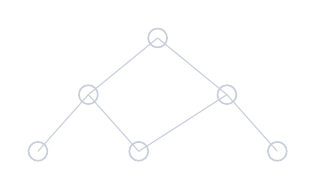
\begin{tikzpicture}[scale=0.8]
  \foreach \x/\y in {0/0, -1.1/-0.9, 1.1/-0.9, -1.9/-1.8, -0.3/-1.8, 1.9/-1.8}
    {\node[circle, draw=d7rule, fill=white, line width=0.6pt,
           minimum size=2.4mm, inner sep=0pt] at (\x,\y) {};}
  \draw[draw=d7rule] (0,0) -- (-1.1,-0.9) -- (-1.9,-1.8);
  \draw[draw=d7rule] (-1.1,-0.9) -- (-0.3,-1.8);
  \draw[draw=d7rule] (0,0) -- (1.1,-0.9) -- (1.9,-1.8);
  \draw[draw=d7rule] (1.1,-0.9) -- (-0.3,-1.8);
\end{tikzpicture}

\vspace{22pt}
{\sffamily\footnotesize\color{d7slate}
 \textsc{the durable7 field guide}\par
 \vspace{4pt}
 Every operation returns a new version\\and leaves the old one untouched.\par}
\end{center}
\vfill

\end{document}
